\documentclass[graybox,envcountchap,sectrefs]{svmono_mod}
%\documentclass[envcountsame,envcountchap]{svmono}

% choose options for [] as required from the list in the Reference Guide
\usepackage{amsmath}
\usepackage{amsfonts}
\usepackage{amssymb}
\usepackage{mathptmx}
\usepackage{helvet}
\usepackage{courier}
%
\usepackage{type1cm}         
\usepackage{makeidx}         % allows index generation
\usepackage{graphicx}        % standard LaTeX graphics tool
                             % when including figure files
\graphicspath{{Figures/}}
\usepackage{multicol}        % used for the two-column index
\usepackage[bottom]{footmisc}% places footnotes at page bottom
\usepackage{array,booktabs,calc}

\usepackage{listings}
\usepackage[final]{pdfpages}
% see the list of further useful packages in the Reference Guide

\usepackage{enumerate}

\usepackage[mode=buildnew]{standalone}
\usepackage{etoolbox}

\usepackage{tikz,pgfplots}
\usetikzlibrary{arrows.meta,quotes, positioning, calc}
% Definición de estilos para los bloques
\tikzset{
    block/.style = {draw, rectangle, minimum height=3em, minimum width=3em},
    sum/.style = {draw, circle, node distance=1cm},
    input/.style = {coordinate},
    output/.style = {coordinate}
}

\usepackage{capt-of}

% Some modifications
\input{format.tex}
% Macros for easier typing
%%%%%%%%%%%%%%%%%%%%%%%%%%%%
%%% Definiciones de comandos

%%% Operadores de decision
\def\dunodcero{\,\, \underset{D=0}{\overset{D=1}{\gtrless}}\,\,}
\def\dceroduno{\,\, \underset{D=1}{\overset{D=0}{\gtrless}}\,\,}
%\def\dunodcero{\begin{array}{c} D=1 \\ \gtrless \\ D=0 \end{array}}
%\def\dceroduno{\begin{array}{c} D=0 \\ \gtrless \\ D=1 \end{array}}

%%% Abreviaturas para PFA, PM  y PD.
\newcommand{\pfa}{P_{\text{FA}}} 
\newcommand{\pmis}{P_{\text{M}}} 
\newcommand{\pdet}{P_{\text{D}}} 
\newcommand{\appropto}{\mathrel{\vcenter{\offinterlineskip\halign{\hfil$##$\cr \propto\cr\noalign{\kern2pt}\sim\cr\noalign{\kern-2pt}}}}}

%%% Abreviaturas para Estimación
\newcommand{\EE}{\mathbb{E}}
\DeclareMathOperator*{\argmin}{argmin} % no space, limits underneath in displays
\DeclareMathOperator*{\argmax}{argmax} % no space, limits underneath in displays
\newcommand{\sML}{\hat{s}_\text{ML}}
\newcommand{\SML}{\hat{S}_\text{ML}}
\newcommand{\sMAP}{\hat{s}_\text{MAP}}
\newcommand{\SMAP}{\hat{S}_\text{MAP}}
\newcommand{\sMSE}{\hat{s}_\text{MSE}}
\newcommand{\SMSE}{\hat{S}_\text{MSE}}
\newcommand{\sMAD}{\hat{s}_\text{MAD}}
\newcommand{\SMAD}{\hat{S}_\text{MAD}}
\newcommand{\ejw}{e^{j\omega}}

%%% Abreviaturas para filtrado
\newcommand{\x}{{\mathbf x}}
\newcommand{\s}{{\mathbf s}}
\newcommand{\uu}{{\mathbf u}}
\newcommand{\UU}{{\mathbf U}}
\newcommand{\PP}{{\mathbf P}}
\newcommand{\Ruu}{{\mathbf R}_{uu}}
\newcommand{\rux}{{\mathbf r}_{ux}}
\newcommand{\hRuu}{\hat{\mathbf R}_{uu}}
\newcommand{\hrux}{\hat {\mathbf r}_{ux}}
\newcommand{\pp}{{\mathbf r}}
\newcommand{\eye}{{\mathbf I}}
\newcommand{\Normal}{{\mathcal N}}
\newcommand{\bigO	}{{\mathcal O}}

%%% Otras
\newcommand{\px}{p_X(x)}
\newcommand{\py}{p_Y(y)}

%%% Para procesos estocasticos
\newcommand{\jw}{j \omega}
 


\makeindex             % used for the subject index
                       % please use the style svind.ist with
                       % your makeindex program

%%%%%%%%%%%%%%%%%%%%%%%%%%%%%%%%%%%%%%%%%%%%%%%%%%%%%%%%%%%%%%%%%%%%%

\begin{document}

\author{Jer\'onimo Arenas-Garc\'ia, Jes\'us Cid-Sueiro, Vanessa G\'omez-Verdejo, Miguel L\'azaro-Gredilla, and David Ram{\'\i}rez}
\title{Estimation and Detection Theory}
\subtitle{Year 2021-22}
\maketitle

\frontmatter


%%%%%%%%%%%%%%%%%%%%%%%%%%%%%%%
% Chapter: Stochastic processes
\chapter{Stochastic Processes}
%
This document introduces the concept of stochastic process and analyzes some important examples.

\vspace{1.5cm}

%%%%%%%%%%%%%%%%%%%%%%
\section{Introduction}
%%%%%%%%%%%%%%%%%%%%%%

A stochastic process (SP) is a collection of random variables $\{X_n\}$ indexed by time, $n$. Depending on the nature of the time variable, there are two types of SP:
\begin{itemize}
\item \textbf{Continuous-time} SP: when the time variable is a real number ($n \in \mathbb{R}$)
\item \textbf{Discrete-time} SP: when the time variable is an integer ($n \in \mathbb{Z}$).
\end{itemize}

This chapter discusses discrete-time processes only. Thus, unless contrary stated, all SP will be assumed to be discrete.

Depending on the range of the time variable, two types of SP will be considered:
\begin{itemize}
\item \textbf{One-sided} SP: $\{X_n, n \ge 0\}$. A one-sided SP is a sequence of random variables.
\item \textbf{Two-sided} SP: $\{X_n, n\in \mathbb{Z}\}$, the SP is defined for all integer times.
\end{itemize}

%%%%%%%%%%%%%%% 
\begin{example}

Consider the one-sided stochastic process $X_n$ such that, for all $n$, $X_n \in \{-n, n\}$ with $P\{X_n=n\}=P\{X_n=-n\}=\frac12$ and all variables in the collection are mutually independent.

\end{example}
%%%%%%%%%%%%%

A realization of all random variables in an SP defines a signal. For this reason, we can define stochastic processes in the following alternative but equivalent form:

%%%%%%%%%%%%%%%%%%%%%%%%%%%%%%%%%%%%%%
\begin{definition}[Stochastic Process]

A discrete-time stochastic process is a probability measure over a space of (one-sided or two-sided) discrete-time signals.

\end{definition}

%%%%%%%%%%%%%%%
\begin{example}
\label{ex:2signals}
Consider the one-sided stochastic process $X_n$ such that
\begin{align}
X_n = n, 	\quad		\text{for all } n \ge 0
\end{align}
or 
\begin{align}
X_n = -n, 	\quad		\text{for all } n \ge 0
\end{align}
with equal probabilities. Note that the universe set of this SP if finite, containing only two signals.

\end{example}
%%%%%%%%%%%%%


%%%%%%%%%%%%%%%%%%%%%%%%%%%%%%%%%%%%%%%%%%%%%%%%%%%%%
\subsection{Characterization of a stochastic process}

In a discrete-time SP, the time variable is discrete, but the random variables defining the SP can be continuous or discrete. In general, a SP is completely characterized when we can determine the joint distribution $P(X_{n_0},X_{n_1},\ldots, X_{n_{M-1}})$ for any subset of random variables from the process. However, for many SP, the computation of these distributions is often unfeasible. We will pay attention to processes satisfying several properties that simplify the characterization.


%%%%%%%%%%%%%%%%%%%%%%%%%%%%%%%
\section{Independent processes}

%%%%%%%%%%%%%%%%%%
\begin{definition}[Independent process]
A stochastic process $X_n$ is statistically independent (or, simply, independent) if all its random variables are statistically independent, that is, for any integer $M >0$ and any subset of $M$ random variables $X_{n_0}, X_{n_1}, \ldots, X_{n_{M-1}}$ with $n_0<n_1,\ldots < n_{M-1}$ we have
\begin{equation}
\label{def_indep}
P(X_{n_0}, X_{n_1}, \ldots, X_{n_{M-1}}) = \prod_{k=0}^{M-1} P(X_{n_k})
\end{equation}
\end{definition}
%%%%%%%%%%%%%%%%

\textbf{Note}: A quick explanation on the mathematical notation. Eq. \eqref{def_indep} should be interpreted as: the joint distribution of the set of $M$ random variables $X_{n_0}, X_{n_1}, \ldots, X_{n_{M-1}}$ is the product of the marginal distribution of each variable. Thus, for instance, the cumulative distribution functions (CDFs) get factorized as follows:
\begin{equation}
\label{Findep}
F_{X_{n_0}, X_{n_1}, \ldots, X_{n_{M-1}}}(x_{n_0}, x_{n_1}, \ldots, x_{n_{M-1}}) 
	= \prod_{k=0}^{M-1} F_{X_{n_k}}(x_{n_k})
\end{equation}
for any $x_{n_0}, x_{n_1}, \ldots, x_{n_{M-1}}$ in the respective domains of the variables. If all the random variables in the process are continuous, Eq. \eqref{Findep} is equivalent to the factorization of the density functions
\begin{equation}
\label{pdf_indep}
p_{X_{n_0}, X_{n_1}, \ldots, X_{n_{M-1}}}(x_{n_0}, x_{n_1}, \ldots, x_{n_{M-1}}) 
	= \prod_{k=0}^{M-1} p_{X_{n_k}}(x_{n_k})
\end{equation}
Also, if the random variables are discrete, this is equivalent to the factorization of the probability mass functions
\begin{equation}
\label{pmf_indep}
P_{X_{n_0}, X_{n_1}, \ldots, X_{n_{M-1}}}(x_{n_0}, x_{n_1}, \ldots, x_{n_{M-1}}) 
	= \prod_{k=0}^{M-1} P P_{X_{n_k}}(x_{n_k})
\end{equation}

In general, we will use formulations like \eqref{def_indep} instead of \eqref{Findep}, \eqref{pdf_indep}, or \eqref{pmf_indep} to express relationships between distributions, because it is simpler and encompasses all of them.

A particularly interesting case arises when all variables in the SP follow the same distribution.

%%%%%%%%%%%%%%%%%%
\begin{definition}[IID process]

A stochastic process $X_n$ is independent and identically distributed, or IID, if it is independent and all variables in the process follow the same distribution, i.e. $P(X_n)=P(X_m)$. This implies that the CDFs re also identical, i.e., $F_{X_n}(x)= F_{X_m}(x)$, for all $x$ and any $n, m$ in the time domain of the process.
\end{definition}
%%%%%%%%%%%%%%%% 

One of the simplest IID processes is the Bernoulli process.

%%%%%%%%%%%%%%%
\begin{example}
A Bernoulli process $X_n$ with parameter $p$, denoted as ${\cal B}(p)$ is an IID process given by Bernoulli random variables:
\begin{equation}
\label{SP:Bernoulli}
P_{X_n}(x) = p^x (1-p)^{1-x},  \qquad x \in \{0, 1\}
\end{equation}
\end{example}
%%%%%%%%%%%%%

Note that Eq. \eqref{SP:Bernoulli} is equivalent to stating that $P\{X_n=1\} = p$ and $P\{X_n=0\} = 1-p$. Bernoulli and other IID processes are commonly used as building blocks of other, more complex, processes.

%%%%%%%%%%%%%%%
\begin{example}
\label{ejexp}
Figure \ref{fig:noisy_sin} shows 4 realizations of the independent stochastic process $X_n$, where each sample of the process follows a Gaussian distribution with mean and standard deviation equal to $4 \sin\left(0.05 \pi n \right)$. 
%%%%%%%%%%%%%%
%\begin{figure}[htb]
\begin{center}
\includegraphics[width=12cm]{Figures/sp_noisy_sin.png} 
\captionof{figure}{4 realizations of process $X_n$} %  described in example \ref{ejexp}}
\label{fig:noisy_sin}
\end{center}
%\end{figure}
%%%%%%%%%%%%

\end{example}
%%%%%%%%%%%%%

  

%%%%%%%%%%%%%%%%%%%%%%
\section{Random walks}

%%%%%%%%%%%%%%%%%%
\begin{definition}[Simple random walk (SRW)]
Let $B_n \in \{-1, 1\}$ be a one-sided IID process with $P\{B_n=1\}=\frac12$. A simple random walk $\{X_n\}$ is defined by $X_0 = 0$ and
\begin{equation}
X_n = \sum_{k=1}^n B_k,    \qquad n>0
\label{sp:srw_def}
\end{equation}
%%%%%%%%%%%%%%

\end{definition}
%%%%%%%%%%%%%%%%

Note that we can express the random variables in a SRW recursively as
 \begin{equation}
X_n = \sum_{k=1}^{n-1} B_k + B_n = X_{n-1} + B_n,    \qquad  n>0
\label{sp:srw_rec}
\end{equation}
Thus, a SRW is not an independent process. It is not an identically distributed process either, since the domain of the random variables in the process grows with $n$. 
\begin{align}
-n \le X_n \le n
\end{align}
Fig. \ref{fig:sp_srw} shows several realizations of the SRW. Note that the realizations are quite far from the bounds. This is because the probability that $X_n$ is close to $n$ or $-n$ vanishes for large $n$.
%%%%%%%%%%%%%%
\begin{figure}[htb]
\begin{center}
\includegraphics[width=14cm]{Figures//sp_random_walk_1d.png} 
\caption{20 realizations of a simple random walk. The straight lines represent the boundaries of the region containing all possible trajectories. The shaded area covers two standard deviations: all trajectories tend to be inside the gray area around 95\% of the time.}
\label{fig:sp_srw}
\end{center}
\end{figure}
%%%%%%%%%%%%

The mean of the process is given by
\begin{align}
\mathbb{E}\{X_n\} = \sum_{k=0}^n \mathbb{E}\{B_k\} = 0
\end{align}
and, since $B_n$ is IID, the variance is given by
\begin{align}
\text{var}\{X_n\} = \sum_{k=1}^n \text{var}\{B_k\} = n
\end{align}
Therefore, the standard deviation is $\sqrt{n}$ and we can expect from the process to lie between the limits $-\sqrt{n}$ and $\sqrt{n}$ most of the time. This can be expressed more precisely by noting that, since $X_n$ is the sum of $n$ independent random variables with zero-mean and bounded variance and, as a consequence of the central limit theorem, $X_n$ converges in distribution to a zero-mean Gaussian random variable with variance $n$. This implies that, after large $n$, we can expect that $|X_n| < 2\sqrt{n}$ approximately 95\% of time.

%%%%%%%%%%%%%%%%%%%%%%%%%%%%%%%%%%%%%%%%%%%
\subsection{Properties of random walks}

\begin{itemize}
\item \textbf{Independent increment} For all $0 \le n_0 \le n_1 \le n_2 \le n_3$, the random variables $X_{n_1} - X_{n_0}$ and $X_{n_3} - X_{n_2}$ are mutually independent
\item \textbf{Time invariance} For all $h \ge 1$, the SP $Z_n = X_{n+h} - X_h$ is a simple random walk.
\end{itemize}

%%%%%%%%%%%%%%%%%%%%%%%%%%%%%%%%%%%%%%%%%%%
\subsection{Stopping times}

The SRW can be used as a model of the total winning and losses of a fair game. Assume that we play a game based on repeated trials of flipping a coin. Every time the result is 'heads', we win 1 point while we loose 1 point otherwise. By taking $B_n=1$ if the $n$-th toss is 'heads', process $X_n=X_{n-1}+B_n$ is an SRW that accounts for the evolution of the total score with time.

Since the SRW is zero mean, we cannot expect a positive gain after an arbitrary number of steps. One may wonder if there is a way to ensure a positive score by choosing the appropriate stopping time. Let's assume we set an upper and lower limits, $U>0$ and $-L<0$, respectively, such that, when $X_n=U$ or $X_n=-L$, we stop betting. By choosing $L$, we set the maximum loss we can tolerate, by choosing $U$, we set the gains that will make us stop playing.

We define {\em stopping time}, $N$ as the first time where $X_N$ reaches $U$ or $-L$. Note that $N$ is a random variable, because it is a function of the random variables in the SP:
\begin{align}
N = \min\{n \mid X_n = U \text{ or } X_n = -L \} 
\end{align}

Is there a way to select $U$ and $L$ in order to expect a positive gain? To answer this question, let us compute the probability of stopping at level $U$, that is $P\{X_N=U|X_0=0\}$. Thus, defining function
$$
f(i) = P\{X_N = U | X_0 = i\}
$$
our goal is to compute $f(0)$. 

Applying the total probability theorem,
\begin{align}
f(i) =& P\{X_N = U | X_0 = i\}  \nonumber \\
     =& P\{X_1 = i+1 | X_0 = i\} P\{X_N = U | X_0 = i, X_1 = i+1\}   \nonumber \\
      &+ P\{X_1 = i-1 | X_0 = i\} P\{X_N = U | X_0 = i, X_1 = i-1\}   \nonumber\\
     =& \frac12 P\{X_N = U | X_1 = i+1\} + \frac12 P\{X_N = U | X_1 = i-1\} \nonumber\\
     =& \frac12 f (i+1) + \frac12 f(i-1)
\end{align}
Noting, also, that $f(U)=1,$ and $f(-L) = 0$, \textcolor{blue}{we can apply standard methods for solving linear difference equations to find the unique solution
\begin{align}
f(i) = \frac{L+i}{L+U}
\end{align}
so that
\begin{align}
f(0) = P\{X_N = U | X_0 = 0\} = \frac{L}{L+U}
\end{align}}
Thus, the gambler can increase the probability of scoring $U$ points by increasing $L$. However, this implies a higher risk to suffer large temporal losses. The expected gain becomes:
\begin{align}
\EE\{X_N\} = U f(0) - L (1-f(0)) = 0
\end{align}
Thus, \textcolor{blue}{there} is no way to set the bounds $U$ and $L$ in order to expect a positive gain.

%\newpage


%%%%%%%%%%%%%%%%%%%%%%%
\section{Markov Chains}

One important property of the simple random walk is that the effect of the past on the future is summarized only by the current state, rather than the whole history of the process. In other words, the distribution of $X_{n+1}$ depends only on the value of $X_n$ and not on the whole set of values of $X_0, X_1, \ldots, X_n$. A stochastic process with such property is called a \textbf{Markov chain}.

%%%%%%%%%%%%%%%%%%
\begin{definition}[Markov chain]
Let $X_n$ be a one-sided discrete-time SP that, for each $n$, takes value in some discrete set ${\cal S}$, which we call  the \textbf{state space}. \textcolor{blue}{We say that $X_n$ is a Markov chain} if
\textcolor{blue}{\begin{align}
P(X_{n+1} | X_n, X_{n-1}, \ldots, X_0) = P(X_{n+1} | X_n)
\label{SP:markov_chain}
\end{align}}
for all $n > 0$. 

\end{definition}
%%%%%%%%%%%%%%%% 

Note that this definition can be extended to two-sided SP, by conditioning over $\{X_k, k\le n\}$ in the left side of \eqref{SP:markov_chain}.

We will say that an MC is \textbf{finite} if ${\cal S}$ is a finite set. In this case, we usually take the elements of ${\cal S}$ as consecutive integers. For instance, for a state space with $m$ elements, we will take ${\cal S} = \{0, 1, \ldots, m-1\}$ or ${\cal S} = \{1, 2, \ldots, m\}$ under our convenience.

Note that the SRW is a one-sided MC, but it is not finite. 

Any finite MC can be described in terms of the transition probabilities
\begin{equation}
\label{SP:state_probs}
p_{ij} = P\{X_{n+1}=j| X_n=i\}
\end{equation}

All the elements of a MC model can be encoded in a \textbf{transition probability matrix}
\begin{align}
{\bf P} = 
\begin{pmatrix}
p_{00} & p_{01} & \ldots & p_{0,m-1}  \\
p_{10} & p_{11} & \ldots & p_{1,m-1}  \\
\vdots & \vdots & \ddots & \vdots  \\
p_{m-1,0} & p_{m-1,1} & \ldots & p_{m-1,m-1} 
\end{pmatrix}
\end{align}

Using \eqref{SP:state_probs}, it is easy to see that
\begin{align}
\sum_{j \in {\cal S}} p_{ij} = 1
\end{align}
thus, all rows in ${\bf P}$ sum up to one. For this reason, we say that ${\bf P}$ is a \textbf{right-stochastic} matrix. In matrix form, this property can be expressed as
\begin{align}
{\bf P}\mathbb{1}_m = \mathbb{1}_m
\label{sp:psum1}
\end{align}
where $\mathbb{1}_m$ is an all-ones vector with dimension $m$.

Note that, in general, the transition probabilities $p_{ij} $ (and, thus, the transition matrix) may change with time. However, the case of constant probabilities is particularly interesting.

%%%%%%%%%%%%%%%%%%
\begin{definition}[Homogeneous Markov Chain]
A markov chain $X_n$ is homogeneous if the transition probabilities do not depend on time, that is.
\begin{align}
P\{X_{n+1}=j| X_n=i\} = P\{X_{m+1}=j| X_m=i\},   \qquad i \in {\cal S},\quad  j \in {\cal S} 
\end{align}
for any $m$ and $n$ in the time domain of the process.
\end{definition}
%%%%%%%%%%%%%%%%


%%%%%%%%%%%%%%%
\begin{example}[Two-state machine]
A machine can be either working or broken on a given day. If it is working, it will break down in the next day with probability 0.01, and will continue working with probability 0.99. If it breaks down
on a given day, it will be repaired and be working in the next day with probability 0.8, and will continue to be broken down with probability 0.2. We can model this machine by a Markov chain with two states: 0 ("working"), and 1 ("broken down"). The transition probability matrix is given by
$$
\begin{pmatrix}
0.99 & 0.01 \\
0.8 & 0.2
\end{pmatrix}
$$
\end{example}
%%%%%%%%%%%%%

%%%%%%%%%%%%%%%
\begin{example}[SRW]
A simple random walk is an MC. However, since its sample space is infinity, it cannot be described by a transition probability matrix.
\end{example}
%%%%%%%%%%%%%

%%%%%%%%%%%%%%%%%%%%%%%%%%%%%
\subsection{Transition graph}

The transition probability matrix of a given homogeneous MC can be  represented by a directed graph, whose nodes are the states, and and edges from node $i$ to node $j$ represents a transition from state $i$ to state $j$ with nonzero probability. The weight of the edge is the transition probability.

%%%%%%%%%%%%%%%
\begin{example}\label{sp:MC3ex}
The transition graph of an MC given by state space ${\cal S} = \{0, 1, 2\}$ and transition probability matrix
\begin{align}
\label{sp:MC3example}
{\bf P} = \begin{pmatrix}
0.4 & 0.2 & 0.4 \\
0   & 1   & 0 \\
0   & 0   & 1 
\end{pmatrix}
\end{align}
is shown in Figure \ref{fig:sp_mc}.

%%%%%%%%%%%%%%
%\begin{figure}[htb]
  \begin{center}
    \includegraphics[width=4cm]{Figures/MC0_markov_chan_graph.png} 
    \captionof{figure}{The transition graph for the markov chain given by \eqref{sp:MC3example}}
    \label{fig:sp_mc}
  \end{center}
%\end{figure}
%%%%%%%%%%%%

\end{example}
%%%%%%%%%%%%%

%%%%%%%%%%%%%%%%%%%%%%%%%%%%%%%%
\subsection{State probabilities}

The transition probability matrix is useful to compute any probabilities about the state of the process at any given time. For instance, the $n$-th step transition probabilities, defined as $r_{ij}(n) = P\{X_n = j | X_0 = i\}$ can be computed recursively, by applying the total probability theorem, as
\begin{align}
r_{ij}(n) 
	&= \sum_{k \in {\cal S}} P\{X_n = j | X_{n-1} = k,  X_0 = i\} P\{X_{n-1} = k | X_0 = i\}  
	 = \sum_{k \in {\cal S}} r_{ik}(n-1) p_{kj},  \qquad n > 1 
\label{sp:mc_rij_rec}	
\end{align}
Note that $r_{ij}(1)= p_{ij}$. 

Defining the $n$-step transition probability  matrix ${\bf R}_n$ as the matrix with components $r_{ij}(n)$, the recurrent relation \eqref{sp:mc_rij_rec} can be written in matrix form as
\begin{align}
{\bf R}_n = {\bf R}_{n-1}{\bf P}
\end{align}
and, noting that ${\bf R}_1={\bf P}$, we get
\begin{align}
{\bf R}_n = {\bf P}^n
\label{sp:mc_Rn_rec}	
\end{align}

Using these relations we can compute the state probabilities at any given time, given the initial state or the initial state probabilities.

For instance, let ${\bf q}_n$ be the state probability vector at time $n$, that is
\begin{align}
q_{n,i} = P\{X_n = i\},    \quad n \ge 0, \quad {i \in {\cal S}}
\end{align}
then we can express the state probability vector at time $n$ as a function of the initial state probabilities using \eqref{sp:mc_Rn_rec} as
\begin{align}
q_{n,j} &= P\{X_n = j\} 
         = \sum_{i \in {\cal S}} P\{X_n = j | X_0 = i\} P\{X_0 = i\} \nonumber\\
        &= \sum_{i \in {\cal S}}  r_{ij}(n) P\{X_0 = i\}
\end{align}
which, in vector form, can be computed as
\begin{align}
{\bf q}_n = {\bf R}_n^\intercal {\bf q}_0 = \left({\bf P}^\intercal\right)^n {\bf q}_0
\end{align}

%%%%%%%%%%%%%%%%%%%%%%%%%%%%%%%%%%%%
\subsection{Stationary distribution}

%%%%%%%%%%%%%%%%%%
\begin{definition}[Stationary distribution]
A stationary distribution of an MC is a probability distribution over the state space ${\cal S}$ (where $P\{X_0=j\} = \pi_j$) such that
\begin{equation}
\label{sp:mc_stat_def}
{\bf P}^\intercal \bm{\pi} = \bm{\pi}
\end{equation}

\end{definition}
%%%%%%%%%%%%%%%%%%

%%%%%%%%%%%%%%%
\begin{example}
Let ${\cal S} = \mathbb{Z}_m$ and $X_0=0$. Consider the MC $X_n$ such that $X_{n+1}=(X_n+1) \mod m$ with probability $\frac12$ and $X_{n+1} = (X_n-1) \mod  m$ with probability $\frac12$.

The stationary distribution of this MC is $\pi_i = \frac1m$.
\end{example}
%%%%%%%%%%%%%

Note that the vector $\bm{\pi} = (\pi_1, \pi_2, \ldots , \pi_m)^\intercal$ is an eigenvector of ${\bf P}^\intercal$ with eigenvalue 1. Hence the following theorem can be deduced from the Perron-Frobenius theorem.

%%%%%%%%%%%%%%%
\begin{theorem}
If $p_{ij} > 0$ for all $i, j \in {\cal S}$, then there exists a unique stationary distribution of the system. 

Moreover, if ${\bf r}_i(n)$ is the state conditional probability vector with components $r_{ij}(n)$, $j \in {\cal S}$ (i.e., the values in the $i$-th row of ${\bf R}_n$),
\begin{align}
\lim_{n \rightarrow \infty} {\bf r}_i(n) = \bm{\pi}, \qquad \forall i, j \in {\cal S}
\end{align}
\end{theorem}
%%%%%%%%%%%%%

A corresponding theorem is not true if we consider infinite state spaces.

Finite Markov chains can be shown to have at least one stationary distribution. However, if at least one of the transition probabilities is zero, the behavior of the process may depend on the topology of the transition graph:

%%%%%%%%%%%%%%%
\begin{itemize}
\item The stationary distribution may be not unique.
\item The limiting distributions $\lim_{n \rightarrow \infty} {\bf r}_i(n)$ may depend on $i$.
\end{itemize}

%%%%%%%%%%%%%%%
\begin{example}

The MC in example \ref{sp:MC3ex} has at least two limiting distributions: $\bm{\pi}_A = (0, 1, 0)^\intercal$ and $\bm{\pi}_B = (0, 0, 1)^\intercal$. Also, any convex combination of them $\bm{\pi} = \alpha \bm{\pi}_A + (1-\alpha) \bm{\pi}_B$, with $0\le \alpha \le 1$ is a stationary distribution. 

The limiting distributions depend on the initial state: is is easy to verify that 
\begin{align}
\lim_{n \rightarrow \infty} {\bf r}_2(n) &= (0, 0, 1)  \\
\lim_{n \rightarrow \infty} {\bf r}_1(n) &= (0, 1, 0)  \\
\lim_{n \rightarrow \infty} {\bf r}_0(n) &= \left(0, \frac13, \frac23 \right)
\end{align}

\end{example}
%%%%%%%%%%%%%

%%%%%%%%%%%%%%%%%%%%%%%%%%%%%%%%%%%%%%%%%%%%%%%%%%
\subsection{Computing the stationary distribution}

In general, the stationary distributions are all the solutions of the set of equations \eqref{sp:mc_stat_def} with the probabilistic constraint $\mathbb{1}^\intercal \bm{\pi} =1$, that is
\begin{align}
\label{sp:mc_stat_eq}
\begin{pmatrix}
{\bf P}^\intercal - {\bf I}  \\
\mathbb{1}^\intercal   
\end{pmatrix}
\bm{\pi} = 
\begin{pmatrix}
0 \\ \vdots \\ 0 \\ 1
\end{pmatrix}
\end{align}

The system of linear equations given by \eqref{sp:mc_stat_eq} is consistent (it has at least one solution) but overdetermined, because the left matrix has $m+1$ rows but only $m$ columns. In fact, using \eqref{sp:psum1}, it is easy to see that 
\begin{equation}
\mathbb{1}_m^\intercal \left({\bf P}^\intercal - {\bf I}\right)  = {\bf 0}
\end{equation}
so that the rank of ${\bf P}^\intercal - {\bf I}$ is at most $m-1$. Thus, we can remove one of the rows in the matrix (any one of them) to solve the system.

%\newpage


%%%%%%%%%%%%%%%%%%%%%%%%%%%%%%
\section{Stationary Processes}
\footnote{This section is \textcolor{blue}{copyrighted}. It cannot be published or redistributed in any form. It cannot be transformed or used partially without permission of the original authors}
%%%%%%%%%%%%%%%%%%%%%%%%%%%%%%

Stationarity refers to the time invariance of some statistical properties of a stochastic process. We have already seen some forms of time invariance in the previous sections: 

\begin{itemize}
\item The homogeneity of Markov chain, $X_n$, which implies the time invariance of the conditional probabilities: $P(X_n|X_m) = P(X_{n+k}|X_{m+k})$, for any $k \ge 0$, $n \ge m \ge 0$. 
\item The time invariance of IID processes, which implies the invariance of the single-variable marginal distributions, $P(X_{n+k}) = P(X_n)$ for any $h>0$
\item The time invariance property of a SRW, which implies that $P(X_{n+h}-X_h) = P(X_n)$.
\end{itemize}

In this section we introduce two forms of stationarity which are particularly interesting in statistical signal processing applications. In its more restrictive form, stationarity implies the invariance of all joint distributions.

%%%%%%%%%%%%%%%%%%%%%%%%%%%%%%%%%%%%%%
\subsection{Strict-Sense Stationarity}
\label{sec:Stationarity}

%%%%%%%%%%%%%%%%%%
\begin{definition}[Strict-Sense Stationarity]
A stochastic process is said to be Strict-Sense Stationary (or simply SSS) if all joint distributions are invariant to a time shift, that is, for any $N>0$, any sampling times $n_0, \ldots, n_{N-1}$ (in the time domain of the process) and any time shift $m > 0$, 
\begin{equation}
\label{ec:strict}
P(X_{n_0},X_{n_1}, \ldots, X_{n_{N-1}}) = P(X_{n_0 + m}, X_{n_1 +m}, \ldots, X_{n_{N-1}+m})
\end{equation}
\end{definition}
%%%%%%%%%%%%%%%%

Thus, if a stochastic process $X_n$ is SSS, the process $Y_n = X_{n+m}$ defines the same probability measure over the signal space. 

%%%%%%%%%%%%%%%
\begin{example}[Bernoulli process]
\label{Ex:BinaryRandom}

A Bernoulli process, ${\cal B}(p)$ given by \eqref{SP:Bernoulli} is IID, thus, its joint probability mass function has the form
\begin{equation}
P_{X_{n_0},\ldots,X_{n_{N-1}}}(x_0,\ldots,x_{N-1})
    = \prod_{i=0}^{N-1} p^{x_i} (1-p)^{1-x_i}
    = p^{\sum_{i=0}^{N-1}x_i} (1-p)^{N - \sum_{i=0}^{N-1}x_i}
\label{ec:PbOrderN}
\end{equation}
which does not depend on $n_0, \ldots, n_{N-1}$. Thus, the Bernoulli process is SSS. 
 
\end{example}
%%%%%%%%%%%%%

In general, all IID processes are SSS. On the contrary, independent but not identically distributed processes are not SSS. This is the case of non-constant deterministic process, as the following example shows

%%%%%%%%%%%%%%%
\begin{example}[Deterministic process]
\label{Ex:SPdeterministic}

Consider the deterministic process given by $X_n = 2 n$ (with probability 1), that is, for each time $n$, $X_n$ is a discrete random variable with PMF
\begin{equation}
P_{X_n}(k) = \delta[k-2 n]
\end{equation}
Since $P_{X_n}(k)$ depends on $n$, $X_n$ is not SSS.

\end{example}
%%%%%%%%%%%%%

In general, strict stationarity is difficult to check and overly restrictive, and weaker forms of stationarity are more interesting. In the following, we will focus in the invariance of first and second order statistics\footnote{In this document, first and second order statistics refer to the expected value of polynomial functions of a random variable up to degree 2, that, it, the mean, the correlation and other related statistics, like the covariance. This should not be confused with the so called "order statistics".}


%%%%%%%%%%%%%%%%%%%%%%%%%%%%%%%%%%%%
\subsection{First and Second-Order Statistics}
\label{sec:CaracterizProcStoc}

In order to define wide-sense stationarity, we will first define some first and second-order statistics of stochastic processes. We will assume, in general, stochastic processes which can take complex values:


%%%%%%%%%%%%%%%%%%
\begin{definition}[First and second order statistics]
Given stochastic process $X_n$ we define the following statistics:

\begin{itemize}
\item \textbf{Mean}:
\begin{equation}\label{ec:DefMediaProcCont}
  \mu_X[n] = \mathbb{E}\{X_n\}
\end{equation}
\item \textbf{Autocorrelation}:
\begin{equation}
r_X[n_1,n_2] = \mathbb{E}\{X_{n_1}X^*_{n_2}\}
\label{ec:autocorr}
\end{equation}
\item \textbf{Cross correlation}
\begin{equation}
r_{XY}[n_1,n_2] = \mathbb{E}\{X_{n_1}Y^*_{n_2}\}
\end{equation}
\end{itemize}

Given stochastic processes $X_n$ and $Y_n$ with means $\mu_X[n]$ and $\mu_Y[n]$, we define the following joint statistics:
\begin{itemize}
\item \textbf{Cross covariance} between $X_n$ and $Y_n$
\begin{equation}
c_{XY}[n_1,n_2] = \mathbb{E}\{(X_{n_1}- \mu_X[n_1]) (Y_{n_2}-\mu_Y[n_2])^*\}
\end{equation}
\item \textbf{Autocovariance}
\begin{equation}
c_X[n_1,n_2] = \mathbb{E}\{(X_{n_1}- \mu_X[n_1]) (X_{n_2}- \mu_X[n_2])^*\}
\end{equation}
\end{itemize}
\end{definition}
%%%%%%%%%%%%%%%%

Note that $c_X[n, n]$ is the variance of $X_n$. It is easy to verify that the autocovariance and the autocorrelation are related by
\begin{equation}
c_X[n_1,n_2] = r_X[n_1,n_2] - \mu_X[n_1] \mu_X^*[n_2]
\label{SP:cx_vs_rx}
\end{equation}

%%%%%%%%%%%%%%%
\begin{example}[Bernoulli process]
\label{Ex:BinaryRandom2}

For a Bernoulli process, ${\cal B}(p)$, using \eqref{SP:Bernoulli} we get
\begin{equation}
\mu_X[n] = \mathbb{E}\{X_n\} = p,
\label{ec:Mean_b}
\end{equation}
also 
\begin{align}
r_X[n_1,n_2] 
	&= \mathbb{E}\{X_{n_1}X_{n_2}\}
     = \left[\begin{array}{ll}
        \EE\{X_{n_1}^2\}              & \mbox{ if } n_1 = n_2 \\
        \EE\{X_{n_1}\} \EE\{X_{n_2}\} & \mbox{ if } n_1\neq n_2
       \end{array}
      \right]
     = \left[\begin{array}{ll}
        p   & \mbox{ if } n_1 = n_2 \\
        p^2 & \mbox{ if } n_1\neq n_2
      \end{array}
    \right]    \nonumber\\
    &= p^2 + p(1-p) \delta[n_1-n_2]
\label{ec:r_b}
\end{align}
and $c_X[n_1,n_2] = r_X[n_1, n_2]$.

\end{example}
%%%%%%%%%%%%%

%%%%%%%%%%%%%%%
\begin{example}[Deterministic process]
\label{Ex:SPdeterministic2}

Consider the deterministic process in Example \ref{Ex:SPdeterministic}, we have
\begin{equation}
\mu_X[n] = \EE\{X_n\} = \EE\{2n\} = 2n,
\end{equation}
\begin{equation}
r_X[n_1,n_2] = \EE\{X_{n_1} X_{n_2}\} = \EE\{4 n_1 n_2\} = 4 n_1 n_2
\label{RxDeterministic}
\end{equation}
and, using \eqref{SP:cx_vs_rx}
\begin{equation}
c_X[n_1,n_2] = 0
\label{CxDeterministic}
\end{equation}

\end{example}
%%%%%%%%%%%%%


%%%%%%%%%%%%%%%
\begin{example}
\label{Ex:SimpleProc}
Consider the stochastic process $X_n$ given by
\begin{equation}
X_n = (1 + n^2) Y 
\end{equation}
where $Y$ is a real Gaussian random variable with zero mean and unit variance. 

The mean and the autocorrelation of the process can be easily calculated as
\begin{equation}
\mu_X[n] = \EE\left\{Y\right\} \cdot (1 + n^2) = 0
\end{equation}
\begin{equation}
r_X(n,m) = \EE\{X_n X_m\}
         = (1 + n^2) \cdot (1 + m^2) \cdot \EE\left\{Y^2\right\} 
         = (1 + n^2) \cdot (1 + m^2) 
\label{ec:autocorr2}
\end{equation}
Since $X_m$ has zero mean, the autocovariance is equal to the autocorrelation, and the variance is
\begin{equation}
\sigma_X^2[n] = r_n[n, n] = \left(1 + n^2\right)^2
\end{equation}

\end{example}
%%%%%%%%%%%%%

%%%%%%%%%%%%%%%
\begin{example}[Simple Random Walk]
\label{Ex:RandomWalk}

For the SRW $X_n$ given by \eqref{sp:srw_def}, the value of the process at any time $n$ depends on the value of a set of $n$ random variables ($Y_1,\ldots Y_n$). We have seen that the process is zero-mean with variance $n$. The autocorrelation (equal to the autocovariance) can be computed as
\begin{align}
r_X[n_1, n_2] 
	&= \EE\{X_{n_1}X_{n_2}\}  
	 = \sum_{k=1}^{n_1} \sum_{\ell=0}^{n_2} \EE\{Y_k Y_\ell\}  
	 = \sum_{k=1}^{n_1} \sum_{\ell=0}^{n_2} \delta[k - \ell]   \nonumber\\
	&= \min(n_1, n_2)
\label{eq:rx_srw}
\end{align}

\end{example}
%%%%%%%%%%%%%


%%%%%%%%%%%%%%%%%%%%%%%%%%%%%%%%%%%%
\subsection{Wide-Sense Stationarity}
\label{sec:WSS}

We are ready to define a weaker form of stationarity:

%%%%%%%%%%%%%%%%%%
\begin{definition}[Wide-Sense Stationarity]
A two-sided stationary process is Wide-Sense Stationary (or simply WSS) if its mean and autocorrelation functions are invariant to a time shift, that is, for any integers $n, n_1, n_2$ and any time shift $m \in \mathbb{Z}$,
\begin{equation}
\mu_X[n] = \mu_X[n+m]
\end{equation}
and
\begin{equation}
r_X[n_1,n_2] = r_X[n_1 + m, n_2 + m]
\end{equation}
\end{definition}
%%%%%%%%%%%%%%%%

Thus, if a process is WSS, its mean is constant and its autocorrelation only depends on the difference between $n_1$ and $n_2$. For this reason, we will typically use the notation
\begin{equation}\label{ec:defmuwss}
\mu_X = \mu_X[n]
\end{equation}
\begin{equation}\label{ec:defrx}
r_X[n] = r_X[m + n, m]
\end{equation}

Also, combining \eqref{ec:defmuwss} and \eqref{ec:defrx} with \eqref{SP:cx_vs_rx}, it is straighforward to see that the covariance function is also invariant to a time shift, and we can write
\begin{equation}\label{ec:defcx}
c_X[n] = c_X[m + n, m]
\end{equation}


%%%%%%%%%%%%%%%
\begin{example}

Let's go back to the examples from the previous section.
\begin{itemize}
\item \textbf{Bernoulli process}: The Bernoulli process $X_n$ from Example \ref{Ex:BinaryRandom} is SSS, since their joint probability function, \eqref{ec:PbOrderN}, does not depend on the time variables. Consequently, it is also WSS, as can be seen by observing that the average in \eqref{ec:Mean_b} is constant and the autocorrelation in \eqref{ec:r_b} depends on the time difference only.

\item \textbf{Deterministic process}: For the deterministic process $X_n=2n$ in Example \ref{Ex:SPdeterministic}, we have $\mu_X[n]=2n$, which depends on $n$. Thus, it is not WSS. 

\item The process $X_n$ in Example \ref{Ex:SimpleProc} has zero mean (thus, the mean is invariant to a time shift), but the autocorrelation $r_X[n_1, n_2]$ \eqref{ec:autocorr2} cannot be expressed as function of the time difference $n_1 - n_2$ only. Thus, the process is not WSS.

\item \textbf{Simple Random Walk}: The SRW from Example \ref{Ex:RandomWalk} is not stationary since its autocorrelation \eqref{eq:rx_srw} is not invariant to a time shift: for any $m>0$
\begin{align}
r_X[n_1 + m, n_2 + m] &= \min(n_1 + m, n_2 + m) 
    = \min(n_1, n_2) + m = r_X(n_1, n_2) + m   \nonumber\\
    & \neq r_X[n_1, n_2]
\end{align}
\end{itemize}
\end{example}
%%%%%%%%%%%%%

%%%%%%%%%%%%%%%%%%%%%%%%%%%%%%%%%%%%%%%%%%%%%%%
\subsubsection{Properties of stationary processes}

\begin{theorem}

The autocorrelation WSS process $X_n$ satisfies the following properties:
\begin{enumerate}
\item \textbf{Hermiticity}: $r_X[n]=r_X^*[-n]$. 
\item $r_X[0]=\EE\{|X_n|^2\}$.
\item It is \textbf{positive-definite}: for any integer $N>0$ and any coefficients $c_n \in 
\mathbb{C}, n=0,\ldots,N-1$, 
\begin{align}
\label{sp:pos_def}
\sum_{m=0}^{N-1}\sum_{n=0}^{N-1} c_m c_n^* r_X[n-m] \ge 0
\end{align}
\item \textbf{Maximality} at the origin: $|r_X[n]|\le r_X[0]$.
\end{enumerate}
\end{theorem}

\begin{proof}
The hermiticity and property 2 are a direct consequence of the definition. To prove the positive definiteness, note that, for any coefficients $c_n$, we have
\begin{align}
0 \le \EE\left\{\left|\sum_{n=0}^{N-1} c_n X_n\right|^2 \right\}  
  =   \sum_{m=0}^{N-1}\sum_{n=0}^{N-1} c_m c_n^* r_X[n-m] 
\end{align}
The maximality at the origin is a consequence of the positive definiteness: since \eqref{sp:pos_def} is true for any complex coefficients, we can take $c_0=1$, $c_1=c_2=\ldots =c_{n-1}=0$ to get
\begin{align}
(1 + \left|c_n X_n\right|^2) r_X[0] + c_n r_X[n] + c_n^* r_x^*[n] \ge 0
\end{align}
and, taking $c_n = -\frac{r_X^*[n]}{\left|r_X[n]\right|}$ (which implies $\left|c_n\right|^2=1$), we get
\begin{align}
2 r_X[0] - 2 \left|r_X[n]\right\| \ge 0
\end{align}
which completes the proof.
\end{proof}

%%%%%%%%%%%%%%%%%%%%%%%%%%%%%%%%%%%%%
\subsubsection{WSS and SSS processes}

Note that stationarity in the strict sense implies the wide sense stationarity, but the opposite is not generally true: there are SSS processes that are not WSS, as the following example shows:

%%%%%%%%%%%%%%%
\begin{example}
Let $X_n$ be a zero mean stationary stochastic process and $Y_n=(-1)^n X_n$. It is easy to check that
\begin{eqnarray}
\mathbb{E}\{Y_n\} = (-1)^n \mathbb{E}\{X_n\} = 0
\end{eqnarray}
and
\begin{eqnarray}
r_Y[n_1,n_2] = (-1)^{n_1+n_2}r_X[n_2-n_1]
\end{eqnarray}
Since $(-1)^{n_1+n_2}=(-1)^{n_2-n_1}$, it follows
\begin{eqnarray}
r_Y[n_1,n_2] = (-1)^{n_2-n_1}r_X[n_2-n_1]
\end{eqnarray}
which only depends on $n_2-n_1$. Therefore, $Y_n$ is WSS. However, we can check that, for example,
\begin{eqnarray}
\EE\{Y^3_n\} = (-1)^n \mathbb{E}\{X^3_n\}
\end{eqnarray}
which, in general, depends on $n$. For example, if, for all $n$, $X_n$ follows the discrete distribution
\begin{eqnarray}
p_X[k] = \frac{3}{4}\delta[k-1]+\frac{1}{4}\delta[k+3]
\end{eqnarray}
we have $\mathbb{E}\{X_n\}=0$ and $\mathbb{E}\{X_n^3\}= -3/2$, then
\begin{eqnarray}
\EE\{Y^3_n\} = -\frac{3}{2}(-1)^n
\end{eqnarray}
which depends on $n$. Therefore, some statistics from $X_n$ are not invariant to a time shift and, thus, $X_n$ is not SSS.
\end{example}
%%%%%%%%%%%%%

Also, note that all IID processes are SSS, with autocovariance
\begin{align}
c_X[n] = \mathbb{E}\{(X_n-\mu_X)(X_0-\mu_X)^*\} = \sigma_X^2 \delta[n]
\end{align}
If the process is zero mean, we have
\begin{align}
\label{eq:rxwhiteprocess}
r_X[n] = \sigma_X^2 \delta[n]
\end{align}
In general, a SP whose autocovariance is a delta function is said to be white. All zero-mean IID processes are white, but the opposite is not true in general: some white processes may be non IID.

%%%%%%%%%%%%%%%%%%%%%%%%%%%%%%%%%%%%%%%%%%%%%
\subsubsection{Jointly stationary processes.}

The two-side stationary processes $X_n$ and $Y_n$ are said to be jointly stationary \textsl{in the strict sense} if their joint statistical 
properties do not vary with a displacement in time, that is, if, for any values of $N$ and $N'$, any value of $m$ and any instants $n_0,\ldots,n_{N-1}$ and $n_0',\ldots,n_{N'-1}'$,

\begin{align}
P(X_{n_0}, \ldots, & X_{n_{N-1}}, Y_{n_0'}, \ldots, Y_{n_{N'-1}'}) 
           =  P(X_{n_0 + m}, \ldots, X_{n_{N-1} + m}, Y_{n_0' + m}, \ldots, Y_{n_{N'-1}' + m})
\end{align}

Likewise, we will say that $X_n$ and $Y_n$ are jointly wide-sense stationary if both are WSS and for any integer values of $n_1, n_2$ and $m$ we have
\begin{equation}
r_{XY}[n_1,n_2] = r_{XY}[n_1 + m, n_2 + m]
\end{equation}
which allows us to describe the cross-correlation function using a single variable
\begin{equation}
r_{XY}[n] = r_{XY}[m + n, m]
\end{equation}


%%%%%%%%%%%%%%%%%%%%%%%%%%%%%%%%%%%%%%%%%%%%%%%%%%% %%%%%%
\subsection{Linear systems with stochastic inputs}
\label{sec:SistemasEntradasStoc}

Let $X_n$ be a stochastic process that is the input to a linear time-invariant system with impulse response $h[n]$. The output process $Y_n$ is given by
\begin{equation}
Y_n = X_n \ast h[n]
\end{equation}

In general, the statistical characterization of $Y_n$ is not easy, except in particular cases (such as the Gaussian), but we can find some useful expressions for some first and second order moments.

For example, the mean of the output process is
\begin{align}
\mu_Y[n] 
	=& \mathbb{E}\{Y_n\} = \mathbb{E}\{h[n] \ast X_n\}
%	=  E\left\{ \sum_{k=-\infty}^{\infty} h[k]* X_{n-k} \right\}   \nonumber \\
%	=& \sum_{k=-\infty}^{\infty} h[k]*\mathbb{E}\{X_{n-k} \}      
    =  h[n]*\mathbb{E}\{X_n\}                                    \nonumber\\
    =& h[n]*\mu_X[n],
\label{ec:mediaout}
\end{align}
the cross-correlation of the input and output is
\begin{align}
r_{YX}[n_1,n_2] 
	=& \EE\{Y_{n_1} X_{n_2}^*\}
  	= \EE\left\{X_{n_2}^* \sum_{k=-\infty}^{\infty} X_k h[n_1-k] \right\} \nonumber \\
    =& \sum_{k=-\infty}^{\infty} h[n_1-k] r_X[k, n_2] \nonumber \\
    =& h[n_1] \ast r_X[n_1, n_2]
\label{RvuNonStationary}
\end{align}
and the autocorrelation of the output is
\begin{align}
r_{Y}[n_1, n_2] 
   =& \EE\{Y_{n_1} Y_{n_2}^* \}
   =  \EE\left\{Y_{n_1} \sum_{k=-\infty}^{\infty} h^*[k] X_{n_2-k}^* \right\} \nonumber\\
   =& \sum_{k=-\infty}^{\infty} h^*[k] r_{YX}[n_1, n_2 - k]                 \nonumber\\
   =& r_{YX}[n_1, n_2] \ast h^*[n_2]
  \label{RvvNonStationary}
\end{align}
Combining (\ref{RvuNonStationary}) and (\ref{RvvNonStationary}), we get
\begin{equation}
r_Y[n_1,n_2] = h[n_1]*r_X[n_1, n_2]*h^*[n_2]
\label{RvvNonStationary2}
\end{equation}

In the above equation, there are two convolution operations. We must perform the first on the variable $n_1$ and the second on the variable $n_2$. Equations \eqref{ec:mediaout} and \eqref{RvvNonStationary2} show that both the mean and the autocorrelation of the output depend exclusively on the mean and the autocorrelation of the input, respectively, as well as on the impulse response of the system.



%%%%%%%%%%%%%%%%%%%%%%%%%%%%%%%%%%%%%%%%%%%
\subsubsection{Stationary processes.}

We can use the general expressions for the output mean and the output autocorrelation to derive specific expression for  WSS processes. If $X_n$ is stationary, $\mu_X[n]=\mu_X$, and
\begin{equation}
  \mu_Y = \mu_X \sum_{n=-\infty}^{\infty} h[n]
  \label{mediaout_stationary}
\end{equation}

Also, by the properties of the convolution operator, for any $m\in \mathbb{Z}$ we can write
\begin{align}
r_Y[n_1 + m, n_2 + m]
	&= h[n_1]*r_X[n_1 + m, n_2 + m]*h^*[n_2]
	 = h[n_1]*r_X[n_1, n_2]*h^*[n_2]  \nonumber\\
	&= r_Y[n_1, n_2]
\end{align}
and, therefore $Y_n$ is also stationary. In such case, we can express the autocorrelation as a function of a single variable. By calling $n=n_1-n_2$, the cross-correlation of the input and output is
\begin{align}
r_{YX}[n_1, n_2] 
    =& h[n_1] \ast r_X[n_1 - n_2]
    =  \sum_{k=-\infty}^{\infty} h[n_1 - k] r_X[k - n_2]  \nonumber \\
    =& \sum_{k=-\infty}^{\infty} h[n_2 + n - k] r_X[k - n_2]
    =  \sum_{k=-\infty}^{\infty} h[n - k] r_X[k] \nonumber \\
    =& h[n] \ast r_X[n]
  \label{RvuStationary}
\end{align}

Finally, the autocorrelation of the output is
\begin{align}
r_Y[n] 
	=& r_Y[n_1, n_2] = r_{YX}[n_1, n_2] \ast h^*[n_2]   \nonumber \\
  	=& \sum_{k=-\infty}^{\infty} h^*[k] r_{YX}[n_1-n_2+k]  
  	=  \sum_{k=-\infty}^{\infty} h^*[k]
  	   \sum_{\ell=-\infty}^{\infty} h[n+k-\ell] r_X[\ell] \nonumber \\
    =& \sum_{\ell=-\infty}^{\infty} r_X[\ell]
       \sum_{k=-\infty}^{\infty} h^*[k] h[n + k - \ell] 
  	=  r_X[n]*h[n]*h^*[-n] \nonumber \\
  	=& r_X[n]*r_h[n]
  \label{RvvStationary}
\end{align}
where $r_h[n]=h[n]*h^*[-n]$.


%%%%%%%%%%%%%%
\begin{example}
  \label{eg:v_estac_ergod}
Let $X_n$ be a unit variance white process. The stationary process $Y_n$ resulting from passing $X_n$ through a linear and invariant and causal filter, given by the difference equation
  \begin{equation}
    Y_n = 0.6 \cdot Y_{n-1} + X_n
  \end{equation}
is stationary. According to \eqref{ec:mediaout}, since the impulse response of this system is $h[n]=0.6^n u[n]$, the process mean will be, 
\begin{equation}
\mu_Y[n] = h[n]*\mu_X[n] = 0
\label{ec:meanv_mediate}
\end{equation}
and its autocorrelation
\begin{eqnarray}
r_Y[n] = r_X[n]*h[n]*h[-n] = \frac{0.6^{|n|}}{0.64}
\label{ec:Rvv_Rrr}
\end{eqnarray}
\end{example}
%%%%%%%%%%%%%%


%%%%%%%%%%%%%%%%%%%%%%%%%%%%%%%
\subsection{Gaussian processes}
\label{sec:snr}

%%%%%%%%%%%%%%%%%%
\begin{definition}[Gaussian Process]
A real SP $X_n$ is a Gaussian Process (GP) if, for any value of $N$ and any arbitrary set of $N$ time instants $\{n_0,\ldots, n_{N-1}\}$, the pdf of order $N$, 
\begin{equation}
p_{X_{n_0},\ldots, X_{n_{N-1}}} (x_0,\ldots,x_{N-1})
\end{equation}
is Gaussian.
\end{definition}
%%%%%%%%%%%%%%%%

Gaussian processes have several interesting properties:
\begin{enumerate}
\item Since the parameters of the (multidimensional) Gaussian distribution are the mean and the covariance matrix, any GP is completely characterized by its mean and its autocorrelation function.
\item Thus, if a GP is WSS, it is SSS.
\item Since any linear combination of Gaussian random variables is Gaussian, if a GP is the input to a linear time-invariant system, the output is also GP characterized by the output mean and the output autocorrelation driven by Eqs. \eqref{ec:mediaout} and \eqref{RPromOut}.
\end{enumerate}

%We can further define jointly Gaussian processes: two Gaussian processes $X_n$ and $Y_n$ are jointly Gaussian if for any values of $N$ and $M$ and any arbitrary sets of time instants $\{n_0,\ldots, n_{N-1}\}$ and $\{k_0,\ldots k_{M-1}\}$, the density function of order probability $N+M$
%\begin{equation}
%p_{X_{n_0},\ldots,X_{n_{N-1}}, Y_{k_0}, \ldots, Y_{k_{M-1}}}(x_0, \ldots, x_{N-1}, y_0, \ldots, y_{M-1})
%\end{equation}
%is Gaussian.
%
%In joint Gaussian processes correlation and statistical independence are equivalent properties, since the joint probability density functions are multidimensional Gaussian.

%%%%%%%%%%%%%%%%%%%%%%%%%%%%%%%%%%%
\subsection{Power Spectral Density}
\label{sec:PowerSpectralDensity}

The Power Spectral Density is the basic tool to extend the Fourier Analysis of signals to stochastic processes. 

Since the realizations of a stochastic process are signals, it is tempting to define the Fourier Transform of a process
stochastic $X_n$ as a new process whose realizations are the Fourier transforms of the realizations of $X_n$, $x_n$. However, there is an insurmountable difficulty in this definition: the realizations of the stationary stochastic processes are signals of finite and non-zero average power and infinite energy and, therefore, they do not have a Fourier Transform.

However, in general, the Fourier Transform of a truncated process (limited in time) can be computed. Let $X_n$ be a stochastic process of mean $\mu_X[n]$ and autocorrelation $r_X[n_1, n_2]$, and consider the truncated process $X_{N,n}$ given by
\begin{equation}
  X_{N,n} = \left\{\begin{array}{ll}
      X_n, & \text{  if } |n| \leq N \\
      0,   & \text{  if } |n| > N    \\
    \end{array}
  \right.
\end{equation}

The Fourier Transform of $X_{N,n}$, given by
\begin{equation}
X_N\left(e^{\jw}\right)
	= \sum_{n=-\infty}^\infty X_{N,n} e^{-\jw n}
    = \sum_{n=-N}^N X_n e^{-\jw n}
\end{equation}
is, in turn, a stochastic process of mean
\begin{equation}
\mathbb{E}\{X_N\left(e^{\jw}\right)\} 
	= \sum_{n=-N}^N \mu_X[n] e^{-\jw n}
\end{equation}
and squared mean
\begin{equation}
\mathbb{E}\left\{\left|X_N\left(e^{\jw}\right)\right|^2\right\} 
	= E\left\{\left|\sum_{n=-N}^N X_n e^{-\jw n} \right|^2 \right \}
\label{PMdeUT}
\end{equation}

If the process is stationary, the mean quadratic value grows indefinitely with $N$ until it becomes infinity, but we can avoid this effect by normalizing \eqref{PMdeUT} with respect to the length of the integration interval, $2N$. We define the \textsl{power spectral density} or
PSD of a stochastic process to the limit of the expression above.

%%%%%%%%%%%%%%%%%%
\begin{definition}[Power Spectral Density]
The power spectal density (PSD) of a stochastic process $X_n$ is defined as
\begin{equation}
S_X(e^{\jw}) = \lim_{N \rightarrow \infty} \frac{1}{2N+1} \mathbb{E}\{|X_N(e^{\jw})|^2\}
\label{defDEP}
\end{equation}
\end{definition}
%%%%%%%%%%%%%%%%

Note that, by definition, the PSD is always real and not negative:
for all $\omega$,
\begin{equation}
S_X\left(e^{\jw}\right) \ge 0
\end{equation}
Also, by the properties of the Fourier Transform, the PSD of a real stochastic process is an even function.

The expression in \eqref{defDEP} is not practical, but we can find an alternative expression for stationary processes, that allows to compute the PSD using the autocorrelation, using a classical result from Wiener and Khinchine that we state without proof.

%%%%%%%%%%%%%%%
\begin{theorem}[Wiener-Khinchine theorem]

If $X_n$ is WSS and $r_X[n]$ is absolutelly summable, 
\begin{equation}
S_X\left(e^{\jw}\right) = \sum_{n=-\infty}^{\infty} r_X[n] e^{-\jw n}
\label{DEPEst}
\end{equation}

\end{theorem}
%%%%%%%%%%%%%

%
%Developing the expression \eqref{PMdeUT}
%\begin{align} 
%\mathbb{E}\{|X_T(e^{\jw})|^2\} 
%	=& E\left\{ \sum_{n_1=-N}^N X_{n_1}   e^{-\jw n_1} 
%	            \sum_{n_2=-N}^N X_{n_2}^* e^{\jw n_2} \right\}
%       \nonumber\\
%  	=& \sum_{n_1=-N}^N \sum_{n_2=-N}^N \mathbb{E}\{X_{n_1} X_{n_2}^* \} e^{-\jw (n_1-n_2)}     \nonumber\\
%  	=& \sum_{n_1=-N}^N \sum_{n_2=-N}^N r_X[n_1, n_2] e^{-\jw(n_1 - n_2)}
%  \label{PMofUT2}
%\end{align}
%thus
%\begin{equation}
%S_X\left(e^{\jw}\right) 
%	= \lim_{N\rightarrow \infty} 
%		\frac{1}{2N+1} \sum_{n_1=-N}^N \sum_{n_2=-N}^N r_X[n_1, n_2] e^{-\jw(n_1-n_2)}
%\label{DEPvsR}
%\end{equation}
%and, making the change of variable $n=n_1-n_2$, we get
%\begin{equation}
%S_X\left(e^{\jw}\right) 
%	= \lim_{N\rightarrow \infty} 
%		\frac{1}{2N+1} \sum_{n_2=-N}^N \sum_{n=-N-n_2}^{N-n_2} r_X[n_2+n, n_2] e^{-\jw n} 
%\label{DEPvsR2}
%\end{equation}
%
%Under certain restrictions on the autocorrelation function, we can simplify this expression until we arrive at
%\begin{equation}
%S_X(e^{\jw}) = \sum_{n=-\infty}^{\infty} \overline{R}_X[n] e^{-\jw n}
%\label{DEPvsRgeneral}
%\end{equation}
%where
%\begin{equation}
%\overline{R}_X[n] = \lim_{N \rightarrow \infty} \frac{1}{2N+1} \sum_{k=-N}^N r_X[k + n, k] 
%\label{Raverage}
%\end{equation}
%This result is known as the Wiener-Khinchine Theorem.  %, and is developed in Appendix \ref{sec:twk}.
%
%We will now analyze this result for the stationary processes.
%
%%%%%%%%%%%%%%%%%%%%%%%%%%%%%%%%%%%%%
%\subsubsection{Stationary processes.}
%
%If the process $X_n$ is WSS, $r_X[k+n, k] = r_X[n]$ and, therefore, $\overline{R}_X[n] = r_X[n]$, so that
%\begin{equation}
%S_X\left(e^{\jw}\right) = \sum_{n=-\infty}^{\infty} r_X[n] e^{-\jw n}
%\label{DEPEst}
%\end{equation}

Therefore, the power spectral density of a stationary process $X_n$ is equal to the Fourier Transform of its autocorrelation function and, conversely
\begin{equation}\label{ec:dep2}
r_X[n] = \frac{1}{2\pi} \int_{-\infty}^\infty S_X(e^{\jw}) e^{\jw n} d\omega
\end{equation}
%so that
%\begin{equation}\label{ec:dep3}
%\EE\{|X_n|^2\} = r_X[0] = \frac{1}{2\pi} \int_{-\infty}^\infty S_X\left(e^{\jw}\right) d\omega
%\end{equation}


\begin{example}{White processes}

If $X_n$ is a white WSS process with autocorrelation $r_X[k]=\sigma_X^2\delta[k]$, its power spectral density is constant at all frequencies.
\begin{eqnarray}
S_X(e^{\jw}) &=& \sigma_X^2
\end{eqnarray}
\end{example}


%%%%%%%%%%%%%%%%%%%%%%%%%%%%%%%%%%%%%%%%%%%%%%%%%%%%%%%%%%%%%%%%%%%%%%
\subsubsection{Power spectral density at the output of linear systems}

It is interesting to analyze the power spectral density of stochastic processes that pass through linear filters. Starting from the expression for the output autocorrelation obtained in \eqref{RvvNonStationary2}, we can write
\begin{eqnarray}
r_Y[n] =&  r_X[n] * h[n] * h^*[-n]
\label{RPromOut}
\end{eqnarray}
and applying the convolution property to (\ref{RPromOut}), we get
\begin{equation}
S_Y\left(e^{\jw}\right) = S_X\left(e^{\jw}\right) \left| H\left(e^{\jw}\right) \right|^2
\label{depout}
\end{equation}


%%%%%%%%%%%%%%%%%%%%%%%
\subsection{Ergodicity}
\label{sec:Ergodicity}

If the expected value of a random variable $X$ is unknown, it can be estimated as the sample average of $K$ independent realizations $x_0,\ldots, x_{K-1}$
\begin{equation}
\EE\{X\} \approx \frac{1}{K} \sum_{k=0}^{K-1} x_k
\end{equation}
This estimation is supported by the (weak and strong) laws of large numbers, that guarantee, under quite general conditions, the convergence of the sample average to the mean as the number of samples goes to infinity.

We can estimate the mean of a stochastic process in the same way, by averaging multiple realizations. However, in many practical applications, this is not possible because only a single sample of the process is available.

If a stochastic process $X_n$ is WSS, the mean is constant, and we can try to estimate it as the average of all samples from a single realization. Thus, we may wonder if time averages of the SP converge to the mean. A process satisfying this property is called mean-ergodic.

%%%%%%%%%%%%%%%%%%
\begin{definition}[Mean-ergodicity]

A WSS process $X_n$ with mean $\mu_X$ is mean-ergodic if the time average
\begin{equation}
  S_N = \frac{1}{2N + 1} \sum_{n=-N}^N X_n
\end{equation}
converges in squared mean to the mean, $\mu_X$, that is
\begin{align}
\lim_{N \rightarrow \infty} \mathbb{E}\left\{\left| S_N - \mu_X \right|^2\right\} = 0
\label{sp:ergod_cond}
\end{align}

\end{definition}
%%%%%%%%%%%%%%%%

Note that $S_N$ is itself a random variable with the same mean as the process
\begin{equation}
\EE\{S_N\} = \frac{1}{2N+1} \sum_{n=-N}^N \EE\{X_n\} = \mu{}_X
\end{equation}
and the expectation in \eqref{sp:ergod_cond} is the variance. Expanding the expression of this variance, it is straightforward to obtain the following condition for ergodicity:

%%%%%%%%%%%%%%%
\begin{theorem}

A WSS process $X_n$ with mean $\mu$ is mean-ergodic iff
\begin{align}
\lim_{N \rightarrow \infty} \frac{1}{(2N+1)^2} \sum_{n=-N}^N\sum_{m=-N}^N  c_X[n-m] = 0
\label{AverageVar0}
\end{align}

\end{theorem}
%%%%%%%%%%%%%

%%%%%%%%%%%%%
\begin{proof}

Noting that
\begin{align}
\EE\{|S_N - \mu_X|^2\} 
    =& \EE\left\{\left| \frac{1}{2N+1} \sum_{n=-N}^N (X_n-\mu_X) \right|^2 \right\} =                \nonumber\\
    =& \frac{1}{(2N+1)^2} \sum_{n=-N}^N \sum_{m=-N}^N \EE\{(X_n-\mu_X)(X_m^*-\mu_X^*) \}  \nonumber\\
    =& \frac{1}{(2N+1)^2} \sum_{n=-N}^N \sum_{m=-N}^N  c_X[n-m]
\label{AverageVar1}
\end{align}
the proof is completed.
\end{proof}
%%%%%%%%%%%

We can use the above theorem to state a sufficient condition for ergodicity, that is satisfied by many WSS processes of practical interest:

%%%%%%%%%%%%%%%
\begin{theorem}

If the covariance function of a WSS process $X_n$ is absolutely summable, that is
\begin{equation}
  \label{eq:ergodicmean1}
  \sum_{n=-\infty}^{\infty} |c_X[n]| <\infty
\end{equation}
the process is mean-ergodic.

\end{theorem}
%%%%%%%%%%%%%

%%%%%%%%%%%%%
\begin{proof}

Since $c_X[n]$ is absolutely summable, $B=\sum_{n=-\infty}^{\infty} |c_X[n]|$ is finite, and we can use $B$ to upper bound the variance in \eqref{AverageVar1} as
\begin{align}
\left|\EE\{|S_N - \mu_X|^2\} \right|
    \le & \frac{1}{(2N+1)^2} \sum_{n=-N}^N\sum_{m=-N}^N  \left|c_X[n-m]\right|
    \le   \frac{1}{(2N+1)^2} \sum_{n=-N}^N B
    =     \frac{B}{2N+1} 
\label{AverageVar2}
\end{align}
Since the upper bound converges to zero for large $N$, the process in mean-ergodic.
\end{proof}
%%%%%%%%%%%

Note that all white processes (and, in particular, IID processes) satisfy \eqref{eq:ergodicmean1}. Thus, they are mean-ergodic.


%%%%%%%%%%%%%%%
\begin{example}\label{ex:ergodic}

Consider the stationary process given by the causal recursive filter $X_n = 0.8 X_{n-1} + Z_n$, where the input, $Z_n$, is a Gaussian IID process of unit variance. It is easy to see that the impulse response of the filter is $h[n] = 0.8^n \cdot u[n]$, where $u[n]$ is the step function. Thus, $X_n$ is a zero-mean stationary process with autocovariance given by \eqref{RvvStationary}, which is equal to
\begin{align}
c_X[n] =& \frac{0.8 ^{|n|}}{0.36} 
\end{align}
Since the autocovariance vanishes for $|k|>1$,the process is mean-ergodic. Figure \ref{fig:ergodicity} represents the first samples (from $n=0$ to $n=79$) of 5 realizations. The average of 1000 realizations is represented in the lower part. The 80 sample average of each realization is shown on the right margin. As a consequence of stationarity, the average signal in the bottom approaches a constant signal around the mean, which is zero. As a consequence of the ergodicity, the averages of each signal also approaches the mean.

%%%%%%%%%%%%%%%
%\begin{figure}[htb]
\begin{center}
\includegraphics[width=12cm]{Figures/sp_ergodicity.png}
\captionof{figure}{5 realizations of the stochastic process of the example \ref{ex:ergodic} (top), the average of 1000 realizations (bottom) and the averages of the represented samples (right). Because of the stationarity, the average signal (at the bottom) approaches a to a zero signal, which is mean of the process. Because of the ergodicity, time averages also approximate the mean.}
\label{fig:ergodicity}
\end{center}
%\end{figure}
%%%%%%%%%%%%

\end{example}
%%%%%%%%%%%%%






%%%%%%%%%%%%%%%%%%%%%%%%%%%%%%%%%%%%%%%%%%%%%%%%%
\subsubsection{Ergodicity in the autocorrelation}

In a similar way, ergodicity is defined in autocorrelation. A WSS process $X_n$ is autocorrelation-ergodic if
\begin{equation}
\label{ec:autocorr_ergodic}
r_N = \frac{1}{2N+1}\sum_{m=-N}^{N} X_{m+n} X_m^*
\end{equation}
converges to $r_X[n]$ in squared mean. In general, $X_n$ is autocorrelation-ergodic if, for every value of $m$, the process $Z_n[m] = X_{m + n} X_m^*$ is mean-ergodic.





%%%%%%%%%%
%\appendix
%%%%%%%%%%
%
%%%%%%%%%%%%%%%%%%%%%%%%%%%%%%%%%%%%%
%\section{Teorema de Wiener-Khinchin}
%\label{sec:twk}
%
%Demostraremos aqu'i que \eqref{DEPvsR2} se reduce a \eqref{DEPvsRgeneral}. Para ello supondremos en primer lugar que la
%correlaci'on cruzada entre dos muestras $X(t)$ y $X(t+\tau)$ est'a acotada por un valor que solamente depende de la separaci'on entre
%ellas, de modo que
%\begin{equation}
%|r_X(t+\tau,t)| \le g(\tau)
%\label{eq:acontandorx}
%\end{equation}
%Asimismo, supondremos que la correlaci'on entre muestras decrece ``suficientemente r'apido'' al aumentar su separaci'on, de tal modo
%que
%\begin{equation}
%\int_{-\infty}^{\infty} g(\tau) d\tau < \infty 
%\label{eq:acontandorx2}
%\end{equation}
%lo que garantiza que $g(\tau)$, al ser no negativa, tiene transformada de Fourier.
%
%La integral doble \eqref{DEPvsR2} sobre el dominio cuadrado de anchura $T$ puede expresarse en funci'on de la integral sobre el dominio
%$-T\le t_2 \le T$, como
%\begin{eqnarray}
%S_X(\jw) 
%  &=& \lim_{T\rightarrow \infty}
%  \frac{1}{2T} \int_{-T}^T \int_{-\infty}^{\infty} r_X(t_2+\tau,t_2) e^{-\jw\tau} d\tau dt_2
%  \nonumber\\
%  &-& \lim_{T\rightarrow \infty}
%  \frac{1}{2T} \int_{-T}^T \int_{T-t_2}^{\infty} r_X(t_2+\tau,t_2) e^{-\jw\tau} d\tau dt_2
%  \nonumber\\
%  &-& \lim_{T\rightarrow \infty}
%  \frac{1}{2T} \int_{-T}^T \int_{-\infty}^{-T-t_2} r_X(t_2+\tau,t_2) e^{-\jw\tau} d\tau dt_2
%  \nonumber\\
%  &=& I_0(\jw) - I_1(\jw) - I_2(\jw)
%  \label{DEPvsR3}
%\end{eqnarray}
%donde hemos llamado, $I_0$, $I_1$ e $I_2$, a cada una de las tres integrales de la expresi'on anterior, siguiendo el orden en que
%aparecen. Demostraremos ahora que $I_1$ e $I_2$ se anulan. Para ello, podemos acotar el m'odulo de $I_1$ mediante
%\begin{eqnarray}
%|I_1(\jw)| &=& \left|\lim_{T\rightarrow \infty} 
%    \frac{1}{2T} 
%    \int_{-T}^T \int_{T-t_2}^{\infty} r_X(t_2+\tau,t_2) e^{-\jw\tau} d\tau dt_2
%  \right|
%  \nonumber\\
%  &\le& \lim_{T\rightarrow \infty} 
%  \frac{1}{2T} 
%  \int_{-T}^T \int_{T-t_2}^{\infty} |r_X(t_2+\tau,t_2)| d\tau dt_2
%  \nonumber\\
%  &\le& \lim_{T\rightarrow \infty} 
%  \frac{1}{2T} 
%  \int_{-T}^T \int_{T-t_2}^{\infty} g(\tau) d\tau dt_2
%\end{eqnarray}
%Asimismo, podemos calcular el l'imite de la expresi'on anterior descomponiendo la integral en suma de dos integrales sobre regiones
%disjuntas,
%\begin{eqnarray}
%  |I_1(\jw)| &\le& 
%  \lim_{T\rightarrow \infty} 
%  \frac{1}{2T} 
%  \int_{-T}^T \int_{T-t_2}^{T} g(\tau) d\tau dt_2
%  + \lim_{T\rightarrow \infty} 
%  \frac{1}{2T} 
%  \int_{-T}^T \int_{T}^{\infty} g(\tau) d\tau dt_2
%  \nonumber\\
%  &=& \lim_{T\rightarrow \infty} 
%  \frac{1}{2T} 
%  \int_{-T}^T \int_{T-t_2}^{T} g(\tau) d\tau dt_2
%  + \lim_{T\rightarrow \infty} 
%  \int_{T}^{\infty} g(\tau) d\tau
%  \label{DEPvsR4}
%\end{eqnarray}
%El segundo t'ermino se anula porque el intervalo de integraci'on tiende a 0. El primero se simplifica cambiando el orden de
%integraci'on respecto de las variables $\tau$ y $t_2$. Resulta, en tal caso,
%\begin{eqnarray}
%|I_1(\jw)| \le \lim_{T\rightarrow \infty} 
%  \frac{1}{2T} \int_0^T \int_{T-\tau}^{T} dt_2  g(\tau) d\tau
%  = \lim_{T\rightarrow \infty} 
%  \frac{1}{2} 
%  \int_0^T \frac{\tau}{T} g(\tau) d\tau
%  \label{DEPvsR5}
%\end{eqnarray}
%cuyo l'imite es cero. De un modo completamente an'alogo se concluye que $|I_2(\jw)|=0$. En consecuencia, \eqref{DEPvsR3} se reduce a
%\begin{eqnarray}
%S_X(\jw) 
%  = \lim_{T\rightarrow \infty}
%  \frac{1}{2T} \int_{-T}^T \int_{-\infty}^{\infty} r_X(t_2+\tau,t_2) e^{-\jw\tau} d\tau dt_2
%  \label{ITvsIInf4}
%\end{eqnarray}
%donde podemos intercambiar la integral y el l'imite al estar acotada $r_X(t_2+\tau,t_2)$ mediante \eqref{eq:acontandorx} y
%\eqref{eq:acontandorx2} , quedando finalmente
%\begin{eqnarray}
%S_X(\jw) = \int_{-\infty}^{\infty}
%  \lim_{T\rightarrow \infty}
%  \frac{1}{2T} \int_{-T}^T r_X(t_2+\tau,t_2) dt_2 
%  e^{-\jw\tau} d\tau 
%  \label{ITvsIInfFin}
%\end{eqnarray}
%y de aqu'i, sustiyendo la definici'on de $\overline{R}_X(\tau)$ seg'un \eqref{Rpromedio}, obtenemos \eqref{DEPvsRgeneral}.



%%%%%%%%%%%%%%%%%%%%%%%%%%%%
% Chapter: Estimation theory

%\include{Contents/part0}
\chapter{Statistical Estimation Theory}


%%%%%%%%%%%%%%%%%%%%
% Chapter: Filtering
\chapter{Linear Filtering}
\label{cha:FiltradoLinea}
%\newcommand{\x}{{\mathbf x}}
\newcommand{\s}{{\mathbf s}}
\newcommand{\uu}{{\mathbf u}}
\newcommand{\UU}{{\mathbf U}}
\newcommand{\PP}{{\mathbf P}}
\newcommand{\Ruu}{{\mathbf R}_{uu}}
\newcommand{\rux}{{\mathbf r}_{ux}}
\newcommand{\hRuu}{\hat{\mathbf R}_{uu}}
\newcommand{\hrux}{\hat {\mathbf r}_{ux}}


\newcommand{\pp}{{\mathbf r}}
\newcommand{\eye}{{\mathbf I}}
\newcommand{\Normal}{{\mathcal N}}
\newcommand{\bigO	}{{\mathcal O}}

%\def\dunodcero{\begin{array}{c} D=1 \\ \gtrless \\ D=0 \end{array}}
%\def\dceroduno{\begin{array}{c} D=0 \\ \gtrless \\ D=1 \end{array}}
%\newcommand{\pfa}{P_{\text{FA}}} 
%\newcommand{\pmis}{P_{\text{M}}} 
%\newcommand{\pdet}{P_{\text{D}}} 
%\newcommand{\argmax}[1]{\underset{#1}{\operatorname{argmax}}~}  % Example \argmax{i}f(i)
%\newcommand{\argmin}[1]{\underset{#1}{\operatorname{argmin}}~}


%%%%%%%%%%%%%%%%%%%%%%%%%%
\label{cha:FiltradoLinea}
%%%%%%%%%%%%%%%%%%%%%%%%%

%%%%%%%%%%%%%%%%%%%%%%
\section{Introduction}

A common challenge in estimation involves determining the coefficients of a linear filter with $M$ coefficients based solely on the observation of its inputs and outputs. This task, along with related ones, falls under the generic term 'linear filtering.' In this chapter, we will demonstrate how the techniques described in Chapter \ref{Estimation Theory} can be applied to design ML, MAP, MAD and MMSE estimators for the coefficients of the aforementioned filter. This will also include the estimation of future filter outputs, provided that the corresponding inputs are known.

%%%%%%%%%%%%%%%%%%%%%%%%%%%%%%%
\section{The filtering problem}

Assume that a finite impulse response filter (FIR) $s[n]$, with $s[n]=0$, for $n$ other than $0,1, \ldots, M-1$ is used to filter a signal\footnote{Although the notation $u[n]$ is frequently used to refer to the step function, in this chapter it is used to denote an arbitrary input signal.} $u[n]$. The result is then added to a certain Gaussian noise $\varepsilon[n]$, which is an IID zero-mean stochastic process with variance $\sigma_\varepsilon^2 $ and independent of $s[n]$, giving rise to an observation $x[n]$ (see Figure \ref{fig:linear_filter}). That is, the corresponding entries are
\begin{align}
x[n] &= u[n]*s[n] + \varepsilon[n]     \nonumber\\
     & = u[n]s[0] + u[n-1]s[1] + \ldots + u[n-M+1]s[M-1] + \varepsilon[n].
\end{align}

%%%%%%%%%%%%%%%%%%%
\begin{figure}[htb]  % "htb" shows the location preference: here, up, down
    \centering
    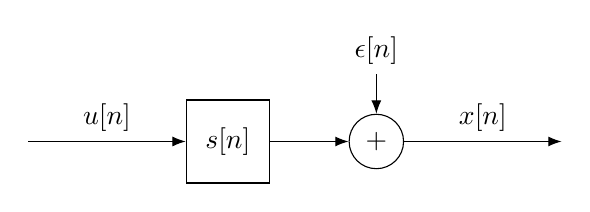
\begin{tikzpicture}[auto, node distance=2cm,>=Latex]
    % Nodos
    \node [input, name=input] {};
    \node [block, right=of input] (filter) {\(s[n]\)};
    \node [sum, right=of filter] (sum) {\(+\)};
    \node [output, right=of sum] (output) {};
    \node [above=0.5cm of sum] (noise) {\(\epsilon[n]\)};
    % Flechas
    \draw [->] (input) -- node {\(u[n]\)} (filter);
    \draw [->] (filter) -- node {} (sum);
    \draw [->] (sum) -- node [name=x] {\(x[n]\)} (output);
    \draw [->] (noise) -- node {} (sum);
\end{tikzpicture}
\caption{The signal model used in this chapter.}
\label{fig:linear_filter}
\end{figure}

For simplicity, we will assume that the input signal starts at $n=0$, that is, $u[n]=0$ for $n<0$. Also, we will assume that it is known; thus, a satistical model for $u[n]$ is unnecessary for our analysis).

The filtering problem consists in estimating the filter $s[n]$ from the input signal and a finite set of $N$ samples from the output, $x[0],\ldots, x[N-1]$. Also, we will tackle the output prediction problem: predicting unobserved values of the output for a given input signal $u[n]$.

Our goal is to solve the filtering problem using the tools from estimation theory developed in Chapter \ref{Estimation Theory}. To do so, we will first represent the target variables (the filter coefficients) and the observations (the output signal) in vector form, and the relation between them using a vector equation. Thus, we will join the nonzero coefficients in an $M$-dimensional vector
\begin{align}
\s &= \begin{bmatrix}
		s[0] \\ s[1] \\ \vdots \\ s[M-1]
      \end{bmatrix}_{M\times 1}.
\end{align}
Also, we will represent any $M$-length window of consecutive input values in vector form as
\begin{align}
\uu[n] &= \begin{bmatrix}
   	    	  u[n] \\ u[n-1] \\ \vdots \\ u[n-M+1]
          \end{bmatrix}_{M\times 1},
\end{align}
we can write
\begin{equation}
\label{eq:signal_model}
x[n] = \uu[n]^\top \s + \varepsilon[n].
\end{equation}

Note that, for any $n$, $\uu[n]$ contains only the input values that are relevant to compute $x[n]$.
% The filtering problem consists in estimating the filter coefficients $\s$ from a set of observed inputs and outputs, as well as estimating the output $x_*$ corresponding to a new input $\uu_*$.

Taking $n=0,1,\ldots,N-1$ in Eq. \eqref{eq:signal_model}, we get a system of $N$ linear equations relating the filter coefficients and the observations. We can join all of them into a single matrix equation by defining the observation vector
\begin{align}
\label{f:defx}
\x &= \begin{bmatrix}
                 x[0] \\ x[1] \\ \vdots \\ x[N-1]
      \end{bmatrix}_{N\times 1},
\end{align}
the input matrix
\begin{align}
\label{f:defU}
\UU &= [\uu[0]~~\uu[1]~\ldots~\uu[M-1]~\ldots~\uu[N-1] ]   \nonumber\\
    &= \begin{bmatrix}
                u[0]  & u[1]   & \ldots & u[M-1] & \ldots & u[N-1] \\
                0     & u[0]   & \ldots & u[M-2] & \ldots & u[N-2] \\
               \vdots & \vdots & \ddots & \vdots & \ldots & \vdots \\
               0      & 0      & \ldots & u[0]   & \ldots & u[N-M] 
       \end{bmatrix}_{M\times N},
\end{align}
and the noise vector
\begin{align}
\label{f:defeps}
\pmb{\epsilon} &= \begin{bmatrix}
                  \varepsilon[0] \\ \varepsilon[1] \\ \vdots \\ \varepsilon[N-1]
                  \end{bmatrix}_{N\times 1},
\end{align}
Using \eqref{f:defx}, \eqref{f:defU} \eqref{f:defeps}, we can write the signal model \eqref{eq:signal_model} as
\begin{framed}
\begin{equation}
\label{eq:signal_model_vec}
\x =\UU^\top \s + \pmb{\epsilon}
\end{equation}
\end{framed}

The filtering problem reduces to the problem of estimating $\s$ given $\x$ knowing \eqref{eq:signal_model_vec} and the noise statistics.

% Versión traspuesta, otra opción razonable de hacer las cosas...
%\begin{equation}
%\UU = 
%\left[ \begin{array}{l}
%\uu[0]  \\
%\uu[1]  \\
%\uu[M-1]  \\
%\vdots  \\
%\uu[N-1]  \\
%\end{array} \right]
%=
%\left[ \begin{array}{llll}
%u[0] & 0 & \ldots & 0 \\
%u[1] & u[0] & \ldots & 0 \\
%u[M-1] & u[M-2] & \ldots & u[0] \\
%\vdots & \vdots & \ddots & \vdots \\
%u[N-1] & u[N-2] & \ldots& u[N-M] \\
%\end{array} \right]
%\end{equation}


%%%%%%%%%%%%%%%%%%%%%
\section{ML solution}
%%%%%%%%%%%%%%%%%%%%%

Eq. \eqref{eq:signal_model} shows that, given $\s$, $x[n]$ is Gaussian with mean
\begin{align}
\EE\{x[n] \mid \s \} = \uu[n]^\top \s + \EE\{\varepsilon[n]\} = \uu[n]^\top \s 
\end{align}
and variance
\begin{align}
\EE\{(x[n]-\uu[n]^\top \s)^2 \mid\s \} = \sigma_\varepsilon^2 
\end{align}
that is, the likelihood function is
\begin{equation}
p(x[n] \mid \s ) = \Normal(x[n] \mid \uu[n]^\top\s, \sigma_\varepsilon^2),
\end{equation}
where the notation $\Normal(x \mid \mu, v) $ is used to refer to the \emph{normal} (Gaussian) pdf of a random variable with mean $\mu$ and variance $v$, evaluated at $x$.

Given $\s$, $x[n]$ depends on $\epsilon[n]$ only, which is an IID process. Thus, all samples from $x[n]$ are independent given $\s$, that is,
\begin{equation}
p_{{\bf X}|{\bf S}}(\x \mid \s) = \prod_{n=0}^{N-1} \Normal(x[n] \mid \uu[n]^\top\s, \sigma_\varepsilon^2) 
           = \Normal(\x \mid \UU^\top\s, \sigma_\varepsilon^2\eye).
\end{equation}

The value of $\s$ that maximizes $p(\x | \s)$ is
\begin{align}
\hat\s_\text{ML} 
   &= \argmax_{\s} p_{{\bf X}|{\bf S}}( \x \mid \s ) 
    = \argmax_{\s} \log p_{{\bf X}|{\bf S}}( \x \mid \s ) \nonumber \\
   &= \argmin_{\s} \frac{1}{2} (\x - \UU^\top\s)^\top(\sigma_\varepsilon^2\eye)^{-1}
                              (\x - \UU^\top\s) 
                + \frac{1}{2} \log|\sigma_\varepsilon^2\eye|+\frac{N}{2}\log(2\pi) 
                \nonumber \\
   &= \argmin_{\s} ||\x - \UU^\top\s||^2     \nonumber \\
\label{sml_comp}
\end{align}

This minimum can be easily obtained by taking the gradient with respect to $\s$, equalizing to zero and clearing, leading to
\begin{framed}
\begin{align}
\hat\s_\text{ML} &= (\UU \UU^\top)^{-1} \UU\x.
\label{sml}
\end{align}
\end{framed}

%%%%%%%%%%%%%%%%%%%%%%%%%%%
\section{Bayesian Solution}
%%%%%%%%%%%%%%%%%%%%%%%%%%%

To obtain a Bayesian estimator of $\s$ it is necessary to know its prior probability distribution, $p(\s)$. A common choice for this distribution is
\begin{equation}
p_{\bf S}(\s) = \Normal(\s | \mathbf{0}, \sigma_s^2\eye),
\end{equation}
since it accommodates any set of real coefficients and assumes they have a zero mean and a dispersion determined by $\sigma_s^2 $. It is also possible to set $\sigma_s^2 \rightarrow \infty$ to approach a uniform distribution. In any case, the use of this prior distribution enables the analytic derivation of the posterior distribution.

Given the likelihood, $p(\x | \s)$, and the prior distribution $p(\s)$, the posterior distribution $p(\s | \x) $ can be obtained. While it is feasible to directly apply Bayes' theorem and simplify the expression as much as possible, this process can be quite tedious. Instead, we will achieve the result in two steps.

First we will determine the joint pdf of $\s$ and $\x$. A simple way to do this is to observe that
\begin{equation}
\begin{bmatrix} \s \\ \x \end{bmatrix} =
	\begin{bmatrix} \eye  \\ \UU^\top          \end{bmatrix} \s + 
	\begin{bmatrix} \bf 0 \\ \pmb{\varepsilon} \end{bmatrix}
\end{equation}
%
that is, vector $[\s^\top~\x^\top]^\top$ is a linear combination of two Gaussian random vectors and, thus, is jointly Gaussian:
\begin{equation}
p_{{\bf S},{\bf X}}(\s,\x) 
	= \Normal\left(\begin{bmatrix} \s \\ \x \end{bmatrix}
                    \, \left| \,	                
	                \begin{bmatrix} {\bf m_S} \\ {\bf m_X} \end{bmatrix},
                    \begin{bmatrix} {\bf V_S}             & {\bf V_{SX}}   \\ 
                                    {\bf V}_{\bf SX}^\top & {\bf V_{X}}   
                    \end{bmatrix}
                    \right.
                    \right)
\end{equation}
where
\begin{align}
{\bf m_S}    &= \EE\{\s\} = {\bf 0}    \\
{\bf m_X}    &= \EE\{\x\} = {\bf U}^\top \EE\{\s\} + \EE\{\pmb{\epsilon}\} = {\bf 0}  \\
{\bf V_S}    &= \text{Var}\{\s\} = \sigma_s^2\eye     \\
{\bf V_{SX}} &= \EE\{\s\x^\top\} = \EE\{\s\s^\top\} \UU + \EE\{\s\pmb{\epsilon}^\top\}  = \sigma_s^2\UU \\
{\bf V_X} &= \EE\{\x\x^\top\} = \UU^\top \EE\{\s\s^\top\} \UU + \EE\{\pmb{\epsilon}\pmb{\epsilon}^\top\}  
           = \sigma_s^2\UU^\top\UU + \sigma_\varepsilon^2 \eye
\end{align}
Therefore,
\begin{align}
p_{{\bf S},{\bf X}}(\s,\x) 
	&= \Normal\left(
	      \begin{bmatrix} \s \\ \x \end{bmatrix}
          \, \left| \,	                
	      \begin{bmatrix} {\bf 0} \\ {\bf 0} \end{bmatrix},
          \begin{bmatrix} \sigma_s^2\eye     & \sigma_s^2\UU \\ 
                          \sigma_s^2\UU^\top & \sigma_s^2\UU^\top\UU + 
                                               \sigma_\varepsilon^2 \eye
          \end{bmatrix}
          \right.
          \right)
\label{eq:jointsx}
\end{align}
From previous chapter, we know that if $p_{{\bf S},{\bf X}}(\s,\x) $ is Gaussian, the conditional distribution $p_{{\bf S}|{\bf X}}(\s \mid \x) $ is also Gaussian, with mean and covariance
\begin{align}
\label{Filt:msx}
{\bf m}_{{\bf S}|{\bf X}} 
      &= {\bf m}_{\bf S} + {\bf V}_{\bf SX}{\bf V_X}^{-1}({\bf x}-{\bf m}_{\bf X})    \nonumber \\
      &= \UU \left(\UU^\top\UU + \tfrac{\sigma_\varepsilon^2}{\sigma_s^2} \eye \right)^{-1}\x \\
\label{Filt:vsx}
{\bf V}_{{\bf S}|{\bf X}} 
      &= {\bf V_S}- {\bf V}_{\bf SX}{\bf V_X}^{-1}{\bf V}_{\bf SX}^\top                \nonumber\\
      &= \sigma_s^2\eye 
       - \sigma_s^2\UU 
         \left(\UU^\top \UU + \tfrac{\sigma_\varepsilon^2}{\sigma_s^2}\eye\right)^{-1} \UU^\top   
\end{align}
The above expressions involve the computation of the inverse of an $N\times N$ matrix, which may be not feasible for large signal records (the computational cost is $\bigO (N^3)$. However, using the {\em matrix inversion lemma} (see the Appendix in Sec. \ref{Sec:mil}), we can obtain the following alternative expressions:
\begin{framed}\begin{align}
\label{Filt:sMMSEgaussMN2}
{\bf m}_{{\bf S}|{\bf X}} &= \PP \UU \x         \\
{\bf V}_{{\bf S}|{\bf X}} &= \sigma_\varepsilon^2 \PP   
\end{align}\end{framed}
where
\begin{framed}
\begin{equation}
\label{Filt:Pdef}
\PP = (\UU\UU^\top  + \tfrac{\sigma_\varepsilon^2}{\sigma_s^2}\eye)^{-1}.
\end{equation}
\end{framed}

Eq. \eqref{Filt:Pdef} involves the inversion of a matrix $M \times M$, which is usually much smaller than $N\times N$. 

Using these expressions, the MMSE, MAP and MAD estimates of $\s$ are:
\begin{framed}
\begin{equation}
\hat\s_\text{MSE} =\hat\s_\text{MAP} =\hat\s_\text{MAD} = \PP  \UU \x
\label{smmse}
\end{equation}
\end{framed}

Also, note that taking $\sigma_\varepsilon^2\rightarrow 0$ (negligible noise) and/or $\sigma_s^2\rightarrow\infty$ (which can be interpreted as assuming an infinitely wide uniform prior) these Bayesian solutions become equivalent to the ML in \eqref{sml}.


%%%%%%%%%%%%%%%%%%%%%%%%%%%%%%%%%%%%%%%%%%%%%%%%%%%%%%%%%%
\subsection{Probabilistic prediction of the filter output}

Once we have resolved several estimators of filter $\s$, we now begin to consider the problem of predicting a new output $x[k]$ at some time $k>N$. Continuing with the Bayesian perspective, we will obtain the posterior pdf of the target variable, $x[k]$, in light of the outputs already observed, $\x$. That is, we aim to calculate $p (x[k] \mid \x)$.

First, it should be noted that $\x, x[k]$ and $\s$ are jointly Gaussian. This follows from Eq. \eqref{eq:jointsx}, which can be extended to any arbitrary number of outputs, including $x[k]$. This necessarily implies that $\x$ and $x[k]$ are jointly Gaussian (when marginalizing $\s$) and finally that $p(x[k] | \x) $ must be Gaussian. Given that
\begin{equation}
x[k] = \uu[k]^\top\s+\varepsilon[k]
\end{equation}
is a linear transformation of $\s$ with independent white noise, we can easily compute the posterior mean and variance, respectively, as follows:
\begin{align}
\EE\{x[k]\mid \x\} &= \uu[k]^\top\EE\{\s\mid \x\} + \EE\{\varepsilon[k] \mid\x\}
                    = \uu[k]^\top\hat\s_\text{MSE}   \\
\text{Var}\{x[k] \mid \x\} 
	&= \EE\left\{\left(\uu[k]^\top \left(\s-\hat\s_\text{MSE}\right) 
	             + \varepsilon[k] \right)^2 \mid\x \right\}   \nonumber\\
    &= \uu[k]^\top \EE\{\left(\s-\hat\s_\text{MSE}\right)\left(\s-\hat\s_\text{MSE}\right)^\top 
                        \mid \x\} \uu[k]
       + \EE\{\varepsilon[k]^2 \mid\x\}    \nonumber\\
    &= \uu[k]^\top {\bf V}_{{\bf S}|{\bf X}} \uu[k] + \sigma_\varepsilon^2   \nonumber\\
    &= \sigma_\varepsilon^2 \uu[k]^\top \PP \uu[k] + \sigma_\varepsilon^2
\end{align}

Therefore, the Bayesian prediction of the output is succinctly given by
%
%\begin{equation}
%p(x[k] \mid \x) = \Normal(x[k] \mid \uu[k]^\top\PP  \UU \x,~~
%                    \sigma_\varepsilon^2+\sigma_\varepsilon^2\uu[k]^\top\PP \uu[k])
%\end{equation}.
\begin{framed}
\begin{equation}
\hat{x}_{\text{MSE} }[k] = \hat{x}_{\text{MAP} }[k] 
                         = \hat{x}_{\text{MAD} }[k]
                         = \uu[k]^\top\hat\s_\text{MSE}.
\label{Filt:xpred}
\end{equation}
\end{framed}

Eq. \eqref{Filt:xpred} shows that the optimal prediction of the output at any time $k>N$ can be computed by passing the input signal $u[n]$ though the filter with the coefficients in the Bayesian estimation of $\s$ (see Fig. \ref{fig:linear_filter2}).

%%%%%%%%%%%%%%%%%%%
\begin{figure}[htb]  % "htb" shows the location preference: here, up, down
    \centering
    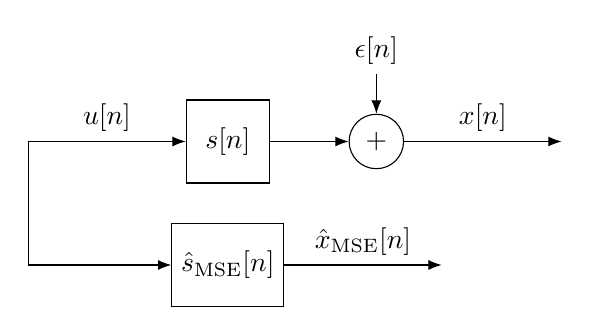
\begin{tikzpicture}[auto, node distance=2cm,>=Latex]
    % Nodos
    \node [input, name=input] {};
    \node [block, right=of input] (filter) {\(s[n]\)};
    \node [sum, right=of filter] (sum) {\(+\)};
    \node [output, right=of sum] (output) {};
    \node [above=0.5cm of sum] (noise) {\(\epsilon[n]\)};
    \node [block, below=0.5 cm of filter] (filterZ) {\(\hat{s}_\text{MSE}[n]\)}; % Nuevo filtro z[n]
    \node [output, right=of filterZ] (outputZ) {}; % Salida de z[n] como y'[n]

    % Flechas
    \draw [->] (input) -- node {\(u[n]\)} (filter);
    \draw [->] (filter) -- node {} (sum);
    \draw [->] (sum) -- node [name=y] {\(x[n]\)} (output);
    \draw [->] (noise) -- node {} (sum);
    \draw [->] (input) |- (filterZ); % Conexión de x[n] a z[n]
    \draw [->] (filterZ) -- node [name=yp] {\(\hat{x}_\text{MSE}[n]\)} (outputZ); % Salida de z[n] 
\end{tikzpicture}
\caption{The best prediction of future values of the output (knowing the input) can be computed by passing the input signal through a filter with the coefficients of the Bayesian estimation of $\s$.}
\label{fig:linear_filter2}
\end{figure}




% Para ello, calculamos
%\begin{align*}
%p(x_*|\x) &= \int_{\mathbb{R}^M} p(x_*, \s | \x) d\s ~~~~\text{      (marginalización de  $\s$)} \\
%&= \int_{\mathbb{R}^M} p(x_*|\s,\x) p(\s|\x) d\s~~~~\text{      (conjunta como producto de  condicional y marginal)} \\
%&= \int_{\mathbb{R}^M} p(x_*|\s) p(\s|\x) d\s~~~~\text{      (dado el filtro $\s$, las salidas son independientes entre sí)}. 
%\end{align*}

%%%%%%%%%%%%%%%%%%%%%%%%%
\section{Online calculus}
%%%%%%%%%%%%%%%%%%%%%%%%%

It is possible to obtain the above solutions online, that is, as new input-output pairs are obtained. While complete calculations could be repeated each time a new sample arrives, there are often more efficient ways to do this.

Note that estimating $\s$ using Eqs. \eqref{sml} or \eqref{smmse} requires inverting an $M \times M$ matrix. This has a cost $\bigO (M^3)$, that is, if we double the size of the filter, $M$ we multiply its computational cost by eight. Suppose now that you want to estimate $\s$ as new input-output pairs are received, that is, we are given first $\{u[0], x[0] \}$, then $\{u[1], x[1] \} $ and so on. In this case, we could reuse the results of the previous estimate to calculate the new updated estimate of $\s$, thus reducing the cost $\bigO(M^3) $ that would have a {\em naive} method that simply recalculates everything again every time a sample arrives.

%%%%%%%%%%%%%%%%%%%%%%%%%%%%%%
\subsection{Bayesian solution}

$\hat\s_\text{MSE}$ can be obtained exactly as more samples are available (i.e. as $N$ increases) without redoing all calculations, by reusing the previous solution. To do this, it is defined
\begin{align}
\PP_N &= (\UU \UU^\top + \tfrac{\sigma_\varepsilon^2}{\sigma_s^2}\eye)^{-1}, \\ \pp_N &= \UU \x
\end{align}
and the following recursive calculation is used (the first equation corresponds to the direct application of the matrix inversion lemma to the $\PP$ update):
\begin{align*}
\PP_{N+1} 
	&= \PP_N -\frac{\PP_N\uu[N+1]\uu[N+1]^\top 
	   \PP_N}{1  +\uu[N+1]^\top  \PP_N\uu[N+1]}  \\
\pp_{N+1} 
    &= \pp_N  +\uu[N+1] x[N+1] \\
\s_{N+1}
    &= \PP_{N+1}\pp_{N+1} ,
\end{align*}
which only has a cost $\bigO(M^2)$ per step (as opposed to applying the complete original equation at each step, which would cost $\bigO(M^3) $). This algorithm is called \emph{recursive least squares} (RLS).

%%%%%%%%%%%%%%%%%%%%%%%%
\subsection{ML solution}

An online approximation to $\hat\s_\text{ML}$ with computational cost $\bigO(M)$ can be obtained just by noting that
\begin{equation}
\hat\s_\text{ML} = \argmax_{\s} p(\x|\s) =  \argmin_{\s} ||\x - \UU^\top\s||^2
\end{equation}
and then use stochastic gradient to minimize $||\x - \UU^\top \s ||^2$.

Notice that
\begin{equation}
||\x - \UU^\top\s||^2 = \sum_{n=0}^{N-1} (x[n] - \uu[n]^\top\s)^2,
\end{equation}
so a gradient descent method would calculate the gradient of that expression and iteratively shift the estimate of the minimum in the opposite direction of the gradient in each step. A descent by stochastic gradient performs the same operation, but considering only one of the additions of the mentioned sum in each step. So,
the updating of coefficients that must be iterated to perform the minimization is in this case
\begin{equation}
\hat\s_{n+1} = \hat\s_n + \mu \left(x[n] - \uu[n]^\top \hat\s_n\right)\uu[n],
\end{equation}
where $\mu$ is an adaptation step that should be ``small enough''. This algorithm is called \emph{least mean squares} (LMS).

%%%%%%%%%%%%%%%%%%%%%%%%
%\section{Wiener filter}
%%%%%%%%%%%%%%%%%%%%%%%%
%
%The Wiener filter $\s_\text{Wiener}$ is the filter that minimizes the expected square error between a desired output $x[n]$ and the output produced when used to filter the input $u[n]$. In this section, both $x[n]$ and $u[n]$ are considered null half signals and $u[n]$ is treated as a stochastic process and not as a deterministic signal, as has been done up to now.
%
%This problem can be posed as a linear estimation problem of minimum mean square error (MMSE), so the formulation of the previous chapter can be used to give rise to the following solution:
%\begin{equation}
%\s_\text{Wiener} = \Ruu^{-1}\rux,
%\end{equation}
%where $\Ruu$ is the autocorrelation matrix of the input signal $u[n]$ and $\rux$ is the cross-correlation vector between $u[n]$ and $x[n]$. Unfortunately, these two quantities are generally unknown, so in most cases, the Wiener filter cannot be calculated. However, it is common to use the above expression using sample estimates for the correlation matrix $\hRuu = \tfrac{1}{N} \UU \UU^\top $ and the cross-correlation vector $\hrux = \tfrac{1}{N} \UU \x$. The result is an approximation to the Wiener filter $\hat\s_\text{Wiener} = \hRuu^{-1}\hrux$ that minimizes the sample quadratic error (often called ``least-squares estimate'') and which matches the ML solution, that is $\hat\s_\text{Wiener} = \hat \s_\text{ML}$.
%
%As the number of samples available for the estimation of the $\Ruu$ and $\rux$ statistics increases, these estimates become more precise, so that $\hat\s_\text {Wiener}$ and therefore $\hat\s_\text{ML}$ match asymptotically with the exact Wiener filter.


%%%%%%%%%%%%%%%%%%
\section{Problems}
%%%%%%%%%%%%%%%%%%

%%%%%%%%%%%%
\begin{prob}
\label{ProbFiltrado}

Consider the sequence
$$
u[1] \ldots u[7] \equiv 0.7,~-0.1,~0.7,~-0.2,~-0.1,~1.5,~-1.1
$$
which is fed as input to a linear filter of three coefficients, $\s = [s_1, s_2, s_3]^\top$. The following elements of the output sequence are known, (corrupted with Gaussian noise of variance 0.25):
$$
x[1] \ldots x[6] \equiv  -0.60,~1.13,~0.57,~0.42,~1.25,~-2.58
$$

\begin {itemize}
\item [a)] What is the ML estimate of $\s$ given the data? % (Wiener filter based on approximate statistics).
\item [b)] Use the obtained filter to predict $x[7]$, $\hat{x}_\text{ML}$.
\item [c)] Calculate the MSE, MAP and MAD estimates of $\s$ assuming that the prior pdf of its components is $s_i \sim \Normal(0,1)$ and that they are independent.
\item [d)] Get the MSE estimate of $x[7]$, $\hat{x}_\text{MSE}$.
\item [e)] Calculate the MSE in prediction b). (That is, the mean of $ (\hat{x}_\text{ML} -x[7])^2$ given the data).
\item [f)] Calculate the MSE in prediction d). (That is, the mean of $(\hat{x}_\text{MMSE} -x[6])^2 $ given the data)
\end{itemize}

\end{prob}
%%%%%%%%%%


%%%%%%%%%%%%%%%%%%%%%%%%%%%%%%%%%%%%%%%%%%%%%%%
\section{Appendix: the matrix inversion lemma}
\label{Sec:mil}

In this section we apply the matrix inversion lemma (also known as the Woodbury matrix identity) to obtain expression. This lemma states that, for any matrices ${\bf U}$, ${\bf C}$, ${bf V}$ and any non-singular matrix ${\bf A}$, 
\begin{align}
\left({\bf A} + {\bf V}{\bf C}{\bf U} \right)^{-1}
    = {\bf A}^{-1} 
    - {\bf A}^{-1}{\bf V} \left({\bf C}^{-1} 
    + {\bf U}{\bf A}^{-1}{\bf V} \right)^{-1} {\bf U}{\bf A}^{-1}
\end{align}
Proving this equality is not difficult: multiplying the right-hand side of the equality by ${\bf A} + {\bf U}{\bf C}{\bf V}$, it is easy to see that the result is the identity matrix.

Taking 
\begin{align}
{\bf A} &= \tfrac{\sigma_\varepsilon^2}{\sigma_s^2} \eye  \\
{\bf C} &= \eye      \\
{\bf V} &= \UU^\top
\end{align}
we get
\begin{align}
\label{Filt:mil}
\left(\UU^\top \UU + \tfrac{\sigma_\varepsilon^2}{\sigma_s^2}\eye \right)^{-1} 
    &= \tfrac{\sigma_s^2}{\sigma_\varepsilon^2}\eye 
	 - \left(\tfrac{\sigma_s^2}{\sigma_\varepsilon^2}\right)^2 \UU^\top 
	   \left(\eye + \tfrac{\sigma_s^2}{\sigma_\varepsilon^2} \UU \UU^\top \right)^{-1} 
	   \UU     \nonumber \\
    &= \tfrac{\sigma_s^2}{\sigma_\varepsilon^2}\eye 
	 - \tfrac{\sigma_s^2}{\sigma_\varepsilon^2} \UU^\top 
	   \left(\UU \UU^\top + \tfrac{\sigma_\varepsilon^2}{\sigma_s^2} \eye \right)^{-1} 
	   \UU   \nonumber\\
    &= \tfrac{\sigma_s^2}{\sigma_\varepsilon^2}\eye 
	 - \tfrac{\sigma_s^2}{\sigma_\varepsilon^2} \UU^\top 
	   \PP \UU
\end{align}
Where $\PP$ is given by \eqref{Filt:Pdef}. Note that, by definition,
\begin{align}
\left(\UU \UU^\top + \tfrac{\sigma_\varepsilon^2}{\sigma_s^2} \eye \right) \PP 
= \PP\left(\UU \UU^\top + \tfrac{\sigma_\varepsilon^2}{\sigma_s^2} \eye \right)  
= \eye 
\end{align}
so that
\begin{align}
\UU \UU^\top \PP = \PP \UU \UU^\top  = \eye - \tfrac{\sigma_\varepsilon^2}{\sigma_s^2} \PP
\end{align}
We will use these equalities below. Using \eqref{Filt:mil} into \eqref{Filt:msx}, we get
\begin{align}
\label{Filt:msx2}
{\bf m}_{{\bf S}|{\bf X}}
      &= \UU \left(\UU^\top\UU + \tfrac{\sigma_\varepsilon^2}{\sigma_s^2} \eye \right)^{-1}\x  
         \nonumber\\
      &= \tfrac{\sigma_s^2}{\sigma_\varepsilon^2} \UU \x 
    	   - \tfrac{\sigma_s^2}{\sigma_\varepsilon^2} 
    	     \UU \UU^\top  \PP 
	     \UU \x  \nonumber\\
      &= \tfrac{\sigma_s^2}{\sigma_\varepsilon^2} \UU \x 
    	   - \tfrac{\sigma_s^2}{\sigma_\varepsilon^2} 
    	     \left(\eye - \tfrac{\sigma_\varepsilon^2}{\sigma_s^2} \PP \right)
	     \UU \x  \nonumber\\
      &= \tfrac{\sigma_s^2}{\sigma_\varepsilon^2} \UU \x 
    	   - \tfrac{\sigma_s^2}{\sigma_\varepsilon^2} \UU \x 
    	   + \PP \UU \x  \nonumber\\
      &= \PP \UU \x  \\
{\bf V}_{{\bf S}|{\bf X}} 
      &= \sigma_s^2\eye 
       - \sigma_s^2\UU \left(\UU^\top \UU + \tfrac{\sigma_\varepsilon^2}{\sigma_s^2}\eye\right)^{-1}
          \UU^\top    \nonumber\\
      &= \sigma_s^2
         \left[  \eye 
               - \UU
                 \left(\tfrac{\sigma_s^2}{\sigma_\varepsilon^2}\eye 
     	             - \tfrac{\sigma_s^2}{\sigma_\varepsilon^2} \UU^\top\PP\UU
                 \right)
                 \UU^\top
         \right]    \nonumber\\
      &= \sigma_s^2
         \left[  \eye
               - \tfrac{\sigma_s^2}{\sigma_\varepsilon^2} \UU \UU^\top
               + \tfrac{\sigma_s^2}{\sigma_\varepsilon^2} \UU \UU^\top\PP\UU
                 \UU^\top
         \right]    \nonumber\\
      &= \sigma_s^2
         \left[  \eye
               - \tfrac{\sigma_s^2}{\sigma_\varepsilon^2} \UU \UU^\top
               + \tfrac{\sigma_s^2}{\sigma_\varepsilon^2} 
                 \left(\eye - \tfrac{\sigma_\varepsilon^2}{\sigma_s^2} \PP\right)\UU
                 \UU^\top
         \right]    \nonumber\\
      &= \sigma_\varepsilon^2 \PP
\end{align}



%%%%%%%%%%%%%%%%%%%%%%%%%%%%%%
% Chapter: Spectral estimation
\chapter{Spectral Estimation}
%\section{Introduction}

This chapter studies a very important estimation problem, which is that of estimating the power spectral density (PSD) of a stationary process. We will consider two families of estimators: 1) classical (or non-parametric) and parametric estimators, which are based on a model for the PSD.

Computing the estimate of $S_x(e^{j \omega})$, which we will denote by $\hat{S}_x(e^{j \omega})$, from an arbitrarily large number of realizations of a stationary process (see Figure \ref{fig:realizations_stochastic_process}) would be a (relatively) easy task. Of course, this is an idealized scenario as we do not have access to all realizations and, even more, we also do not have access to all time samples of the same realization. Thus, the objective in this chapter is to compute $\hat{S}_x(e^{j \omega})$ from $N$ samples of a single realization of the process $x[n]$.

The spectral estimation problem is defined only for wide-sense stationary (WSS) processes for which the mean function is time-independent, that is, $\mu_x = \mu_x[n] = \mathbb{E}[x[n]]$, and the auto-correlation function depends only on the time difference, i.e., $r_{x}[m] = r_{x}[n,n-m] = \mathbb{E}[x[n] x^{\ast}[n-m]]$. For non-stationary processes, the usual practice is to apply the estimators to small windows, since on a local scale we can assume that non-stationary processes are WSS. For instance, this is typically done when analyzing speech signals, which are usually described using non-stationary processes. Moreover, since only one realization is available, the process must be ergodic such that expectations can be substituted by time averages.

\begin{figure}
    \begin{center}
	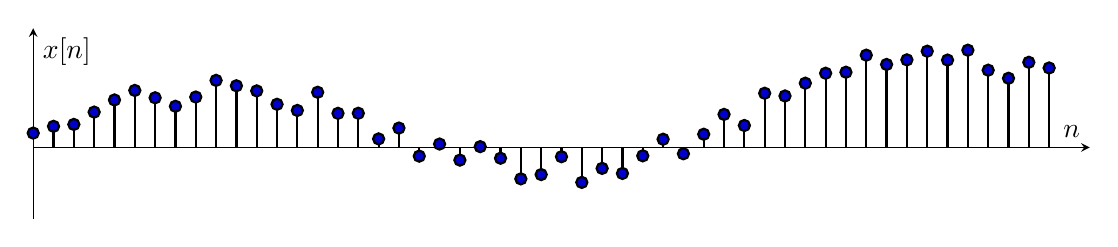
\begin{tikzpicture}
		\begin{axis}[%
		axis x line=middle,
		axis y line=middle,
		ticks=none,
		enlarge x limits=0,
		enlarge y limits=0.15,
		xmin=0,
		xmax=52,
		ymin=-1,
		width=15cm,
		height=4cm,
		domain = 0:50,
		samples = 51,
		xlabel={$n$},
		ylabel={$x[n]$}]
		\addplot+[ycomb,black,thick] {sin(2*180*x/35) + 0.3*rand + x/50 };
		\end{axis}
	\end{tikzpicture}
	\end{center}
    \begin{center}
	\huge{$\vdots$}
	\end{center}
	\begin{center}
	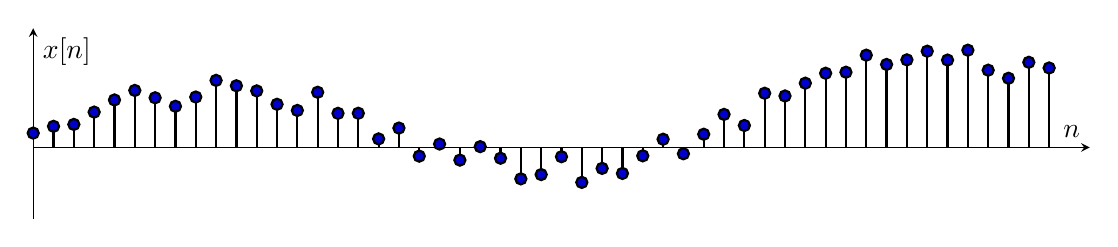
\begin{tikzpicture}
	\begin{axis}[%
		axis x line=middle,
		axis y line=middle,
		ticks=none,
		enlarge x limits=0,
		enlarge y limits=0.15,
		xmin=0,
		xmax=52,
		ymin=-1,
		width=15cm,
		height=4cm,
		domain = 0:50,
		samples = 51,
		xlabel={$n$},
		ylabel={$x[n]$}]
		\addplot+[ycomb,black,thick] {sin(2*180*x/35) + 0.3*rand + x/50};
\end{axis}
\end{tikzpicture}
	\end{center}
\caption{Realizations of a discrete stochastic process}
\label{fig:realizations_stochastic_process}
\end{figure}

\section{Preliminaries: Spectral analysis of deterministic signals}
\label{sec:preliminaries_deterministic_signals}
	
Before going into the spectral analysis of stochastic processes, it is convenient to study the case of deterministic signals, which will help us to understand the concept of spectral resolution. Thus, the problem is to compute the Fourier transform of the deterministic signal $x[n]$. However, this relatively ``simple'' task has two problems. First, we do not have access to the whole signal $x[n]$, but only to a finite record thereof
\begin{equation*}
   x_w[n]  = \begin{cases}
   x[n], & n = 0, \ldots, N-1, \\
   0, & \text{otherwise.}
   \end{cases}
\end{equation*}
Defining now the window
\begin{equation*}
w_{R,N}[n]  = \begin{cases}
1, & n = 0, \ldots, N-1, \\
0, & \text{otherwise,}
\end{cases}
\end{equation*}
we may rewrite $x_w[n] = w_{R,N}[n] x[n]$, which allows us to compute the Fourier transform of $x_w[n]$ as\footnote{In the ``Signals and Systems'' parlance, this Fourier transform is named Discrete Time Fourier Transform (DTFT).}
\begin{equation}
\label{eq:DTFT}
X_w(e^{j \omega}) = \mathcal{F} \left(x_w[n]\right) = \sum_{n = 0}^{N-1} x_w[n] e^{- j \omega N} = \frac{1}{2 \pi} W_{R,N}(e^{j \omega}) \circledast X(e^{j \omega}),
\end{equation}
where $\circledast$ denotes the circular convolution. So, the Fourier transform of the windowed signal, $x_w[n]$, is related to that of $x[n]$ through the Fourier transform of the window $w_{R,N}[n]$, which is given by
\begin{equation*}
W_{R,N}(e^{j \omega}) = e^{-j \omega (N-1)/2} \frac{\sin\left(\frac{\omega N}{2}\right)}{\sin\left(\frac{\omega}{2}\right)} = e^{-j \omega (N-1)/2} P_N(e^{j \omega}),
\end{equation*}
and its amplitude $|P_N(e^{j \omega})|$ is depicted in Figure \ref{fig:FT_rectangularwindow}. As this figure shows, the width of the main lobe is $4 \pi/N$.

\begin{figure}
	\pgfmathsetmacro{\mypi}{3.141592}
	\pgfmathsetmacro{\windowlength}{10}
	\begin{center}
		\begin{tikzpicture}
		\begin{axis}[%
		axis x line=middle,
		axis y line=middle,
		enlarge x limits=0.05,
		enlarge y limits=0.2,
		xtick={-\mypi,-2*\mypi/\windowlength,2*\mypi/\windowlength,\mypi},
		xticklabels={$-\pi$,$-\frac{2\pi}{N}$,$\frac{2\pi}{N}$,$\pi$},
		xmin=-\mypi,
		xmax=\mypi,
		ymin=0,
		ytick=\empty,
		width=10cm,
		height=7.5cm,
		domain = -\mypi:\mypi,
		samples = 512,
		xlabel={$\omega$},
		ylabel={$|P_N(e^{j \omega})|$}]
		%\addplot+[ycomb,black,thick] {x*\mypi};
		\addplot[black,thick] {abs(sin(deg(x*\windowlength/2))/sin(deg(x/2)))};
		\end{axis}
		\end{tikzpicture}
	\end{center}
	\caption{Module of the Fourier transform of the rectangular window}
	\label{fig:FT_rectangularwindow}
\end{figure}

The second issue is that the DTFT in \eqref{eq:DTFT} is a function of a continuous variable. Hence it cannot be computed nor stored in a computer. The solution is simple and consists in discretizing the spectrum, which yields the Discrete Fourier Transform (DFT). Thus, we are only able to compute $X_w(e^{j \omega_k}),$ with $\omega_k = 2 \pi k/N$ and $k = 0, \ldots, N-1$. The DFT is typically computed using the fast Fourier transform (FFT) algorithm. 

The aforementioned procedure based on the DFT/FFT gets only $N$ samples of the spectrum for length-$N$ signals, but we can get more samples by zero-padding the signals, i.e., by simply adding $N_\text{fft} - N$ zeros after the $N$ samples. This procedure increases the number of frequencies but it does not increase the resolution as it does not modify the window.
	
%%%%%%%%%%%%%%%
\begin{example}[Spectral analysis of a complex exponential]
	\label{ex:spectral_analysis_deterministic}
	
	This example considers the spectral analysis of a finite record of a complex exponential, i.e., $x[n] = e^{j \omega_0 n}, n = 0, \ldots, N-1$. Using the DTFT of a complex exponential, given by
\begin{equation*}
X(e^{j \omega}) = 2 \pi \delta(\omega - \omega_0),
\end{equation*}
and $W_N(e^{j \omega})$, $X_w(e^{j \omega})$ becomes
\begin{equation*}
X_w(e^{j \omega}) = e^{-j (\omega - \omega_0) (N-1)/2} \frac{\sin\left(\frac{(\omega - \omega_0) N}{2}\right)}{\sin\left(\frac{\omega - \omega_0}{2}\right)} =  e^{-j (\omega - \omega_0) (N-1)/2} P_N\left(\omega - \omega_0\right),
\end{equation*}
and its magnitude squared is
\begin{equation*}
|X_w(e^{j \omega})|^2 = \left|P_N\left(e^{j (\omega - \omega_0)}\right)\right|^2.
\end{equation*}
Figure \ref{fig:FT_complexexponential} plots, in logarithmic scale, $|X_w(e^{j \omega})|^2$ and $|X_w(e^{j \omega_k})|^2$ for two different values of $N_\text{fft}$.
\begin{figure}
	\pgfmathsetmacro{\mypi}{3.141592}
	\pgfmathsetmacro{\windowlength}{14}
	\pgfmathsetmacro{\myomega}{\mypi/8}
	\begin{center}
		\begin{tikzpicture}
		\begin{axis}[%
		axis x line=bottom,
		axis y line=middle,
		enlarge x limits=0.05,
		enlarge y limits=0.2,
		xtick={-\mypi,\myomega,\mypi},
		xticklabels={$-\pi$,$\omega_0$,$\pi$},
		xmin=-\mypi,
		xmax=\mypi,
		ymin=1e-3,
		ytick=\empty,
		ymode=log,
		width=8cm,
		height=6cm,
		domain = -\mypi:\mypi,
		samples = 512,
		xlabel={$\omega$},
		ylabel={$|X_w(e^{j \omega})|^2$}]
		%\addplot+[ycomb,black,thick] {x*\mypi};
		\addplot[black,thick] {(sin(deg((x-\myomega)*\windowlength/2))/sin(deg((x-\myomega)/2)))^2};
		\addplot+[only marks,mark=*,black,thick,each nth point=32] {(sin(deg((x-\myomega)*\windowlength/2))/sin(deg((x-\myomega)/2)))^2};
		\end{axis}
		\end{tikzpicture}
		\hspace{0.5cm}
		\begin{tikzpicture}
\begin{axis}[%
axis x line=bottom,
axis y line=middle,
enlarge x limits=0.05,
enlarge y limits=0.2,
xtick={-\mypi,\myomega,\mypi},
xticklabels={$-\pi$,$\omega_0$,$\pi$},
xmin=-\mypi,
xmax=\mypi,
ymin=1e-3,
ytick=\empty,
ymode=log,
width=8cm,
height=6cm,
domain = -\mypi:\mypi,
samples = 512,
xlabel={$\omega$},
ylabel={$|X_w(e^{j \omega})|^2$}]
\addplot[black,thick] {(sin(deg((x-\myomega)*\windowlength/2))/sin(deg((x-\myomega)/2)))^2};
\addplot+[only marks,mark=*,black,thick,each nth point=16] {(sin(deg((x-\myomega)*\windowlength/2))/sin(deg((x-\myomega)/2)))^2};
\end{axis}
\end{tikzpicture}
	\end{center}
	\caption{Fourier transform (in logarithmic scale) of a windowed complex exponential}
	\label{fig:FT_complexexponential}
\end{figure}
		
As we have seen in this example, the spectral analysis of deterministic signals depends on two factors. First, the number of available samples, which determines the window and, therefore, the shape of the windowed spectrum. As we have seen in Figure \ref{fig:FT_complexexponential}, the rectangular window has a narrow main lobe at the expense of high secondary lobes. This effect could be reduced by pre-multiplying $x_w[n]$ by a different window, which would reduce the height of the secondary lobes, but it would widen the main lobe.

\end{example}
%%%%%%%%%%%%%

%%%%%%%%%%%%%%%
\begin{example}[Spectral analysis of two complex exponentials]
	\label{ex:spectral_analysis_deterministic_two}
	
	This example considers the spectral analysis of a finite record of the sum of two complex exponential, i.e., $x[n] = e^{j \omega_0 n} + e^{j \omega_1 n}, n = 0, \ldots, N-1$, which will help us to understand the concept of resolution. Using \eqref{eq:DTFT}, we have
	\begin{equation*}
	X_w(e^{j \omega}) = e^{-j (\omega - \omega_0) (N-1)/2} P_N\left(\omega - \omega_0\right)+  e^{-j (\omega - \omega_1) (N-1)/2} P_N\left(\omega - \omega_1\right).
	\end{equation*}
	and its magnitude squared is
	\begin{multline*}
	|X_w(e^{j \omega})|^2 = \left|P_N\left(e^{j (\omega - \omega_0)}\right)\right|^2 + \left|P_N\left(e^{j (\omega - \omega_1)}\right)\right|^2  \\  + e^{j (\omega_0 - \omega_1) (N-1)/2} P_N\left(e^{j (\omega - \omega_0)}\right) P_N\left(e^{j (\omega - \omega_1)}\right)\\ +  e^{- j (\omega_0 - \omega_1) (N-1)/2} P_N\left(e^{j (\omega - \omega_0)}\right) P_N\left(e^{j (\omega - \omega_1)}\right).
\end{multline*}
Taking into account Euler's formula, $|X_w(e^{j \omega})|^2$ can be simplified as
	\begin{multline*}
|X_w(e^{j \omega})|^2 = \left|P_N\left(e^{j (\omega - \omega_0)}\right)\right|^2 + \left|P_N\left(e^{j (\omega - \omega_1)}\right)\right|^2  \\  + 2 \cos \left(\frac{(\omega_0 - \omega_1) (N-1)}{2} \right) P_N\left(e^{j (\omega - \omega_0)}\right) P_N\left(e^{j (\omega - \omega_1)}\right).
\end{multline*}
Figure \ref{fig:FT_twocomplexexponential} plots, in logarithmic scale, $|X_w(e^{j \omega})|^2$ for two different separations between the frequencies of the exponentials. As we can see in this figure, for small frequency separations, it is impossible to identify in the spectrum the two complex exponentials.
	\begin{figure}
		\pgfmathsetmacro{\mypi}{3.141592}
		\pgfmathsetmacro{\windowlength}{14}
		\pgfmathsetmacro{\myomega}{\mypi/8}
		\pgfmathsetmacro{\myomegabis}{3*\mypi/8}
		\pgfmathsetmacro{\myomegabisbis}{1.5*\mypi/8}
		\begin{center}
	\begin{tikzpicture}
\begin{axis}[%
axis x line=bottom,
axis y line=middle,
enlarge x limits=0.05,
enlarge y limits=0.2,
xtick={-\mypi,\myomega,\myomegabis,\mypi},
xticklabels={$-\pi$,$\omega_0$,$\omega_1$,$\pi$},
xmin=-\mypi,
xmax=\mypi,
ymin=1e-3,
ytick=\empty,
ymode=log,
width=8cm,
height=6cm,
domain = -\mypi:\mypi,
samples = 512,
xlabel={$\omega$},
ylabel={$|X_w(e^{j \omega})|^2$}]
\addplot[black,thick] {(sin(deg((x-\myomega)*\windowlength/2))/sin(deg((x-\myomega)/2)))^2 + (sin(deg((x-\myomegabis)*\windowlength/2))/sin(deg((x-\myomegabis)/2)))^2  + 2*cos(deg((\myomega - \myomegabis)*(\windowlength - 1)/2))*(sin(deg((x-\myomega)*\windowlength/2))/sin(deg((x-\myomega)/2)))*(sin(deg((x-\myomegabis)*\windowlength/2))/sin(deg((x-\myomegabis)/2)))};
\end{axis}
\end{tikzpicture}
	\begin{tikzpicture}
\begin{axis}[%
axis x line=bottom,
axis y line=middle,
enlarge x limits=0.05,
enlarge y limits=0.2,
xtick={-\mypi,\myomega,\mypi},
xticklabels={$-\pi$,$\omega_0$,$\pi$},
extra x ticks={\myomegabisbis},
extra x tick labels={$\omega_1$},
extra x tick style={tick label style={yshift=5mm}},
xmin=-\mypi,
xmax=\mypi,
ymin=1e-3,
ytick=\empty,
ymode=log,
width=8cm,
height=6cm,
domain = -\mypi:\mypi,
samples = 512,
xlabel={$\omega$},
ylabel={$|X_w(e^{j \omega})|^2$}]
\addplot[black,thick] {(sin(deg((x-\myomega)*\windowlength/2))/sin(deg((x-\myomega)/2)))^2 + (sin(deg((x-\myomegabisbis)*\windowlength/2))/sin(deg((x-\myomegabisbis)/2)))^2  + 2*cos(deg((\myomega - \myomegabisbis)*(\windowlength - 1)/2))*(sin(deg((x-\myomega)*\windowlength/2))/sin(deg((x-\myomega)/2)))*(sin(deg((x-\myomegabisbis)*\windowlength/2))/sin(deg((x-\myomegabisbis)/2)))};
\end{axis}
\end{tikzpicture}
		\end{center}
		\caption{Fourier transform (in logarithmic scale) of the sum of two complex exponentials}
		\label{fig:FT_twocomplexexponential}
	\end{figure}
	
\end{example}
%%%%%%%%%%%%%

\section{Non-parametric methods in spectral estimation}

In this section, we turn our attention to the case of stochastic signals and, in particular, to the development of non-parametric spectral estimation methods. We will therefore study the periodogram and variations thereof. 

Before proceeding, let us note that throughout this section, we will only consider DTFTs. However, we have to keep in mind that, in practice, we can only compute the DFT (using the FFT algorithm), as we have seen in Section \ref{sec:preliminaries_deterministic_signals}.

\subsection{The periodogram}

Despite the title section, we will start with an estimator known as correlogram, which is based on a first definition of the PSD.
\begin{definition}
	\label{wiener_khinchin}
	Given a WSS process $x[n]$, the power spectral density is defined as
	\begin{equation*}
	S_x(e^{j \omega}) = \mathcal{F}(r_{x}[m]),
	\end{equation*}
	where
	\begin{equation*}
	r_{x}[m] = \mathbb{E}[x[n] x^{\ast}[n-m]],
	\end{equation*}
	is the auto-correlation function of the process $x[n]$.
\end{definition}

Based on Definition \ref{wiener_khinchin}, the first estimator of the PSD is given by
\begin{equation*}
	\hat{S}_x(e^{j \omega}) = \mathcal{F}(\hat{r}_{x}[m]),
\end{equation*}
where $\hat{r}_{x}[m]$ is an estimator of the auto-correlation function. Concretely, we have two alternatives for this estimator: a biased and an unbiased estimator. The biased estimator of the auto-correlation, given the finite length $x[n], n = 0, \ldots, N-1$, is
\begin{equation}
	\label{eq:autocorrelation_biased}
	\hat{r}_{x}^{b}[m] = \frac{1}{N} \sum_{n = m}^{N-1} x[n] x^{\ast}[n-m], \quad m = 0, \ldots, N-1,
\end{equation}
and $\hat{r}_{x}^{b}[m] = \left[ \hat{r}_{x}^{b}[-m] \right]^{\ast}, m = -N+1, \ldots, -1$, whereas the unbiased estimator is
\begin{equation}
	\label{eq:autocorrelation_unbiased}
\hat{r}_{x}^{u}[m] = \frac{1}{N-m} \sum_{n = m}^{N-1} x[n] x^{\ast}[n-m], \quad m = 0, \ldots, N-1,
\end{equation}
and $\hat{r}_{x}^{u}[m] = \left[ \hat{r}_{x}^{u}[-m] \right]^{\ast}, m = -N+1, \ldots, -1$. Consequently, the PSD estimators are
\begin{equation}
\label{eq:correlogram}
\hat{S}_x^{b}(e^{j \omega}) = \mathcal{F}(\hat{r}_{x}^{b}[m]),
\end{equation}
and
\begin{equation*}
\hat{S}_x^{u}(e^{j \omega}) = \mathcal{F}(\hat{r}_{x}^{u}[m]).
\end{equation*}
Actually, only the estimator in \eqref{eq:correlogram}, which is known as the correlogram, is a valid PSD estimator since it ensures $\hat{S}_x^{b}(e^{j \omega}) \geq 0$, whereas $\hat{S}_x^{u}(e^{j \omega}) \not \geq 0$.

The periodogram, which is a term coined by Arthur Schuster in 1898, is based on a second definition of the power spectral density. This definition states that
\begin{equation*}
	S_x(e^{j \omega}) = \lim_{N \rightarrow \infty} \ E \left[\frac{1}{2N -1} \left| \sum_{n = -N+1}^{N-1} x[n] e^{-j \omega n} \right|^2 \right].
\end{equation*}
The periodogram is obtained from the above definition by simply dropping the expectation and considering a finite number of samples, i.e.,
\begin{equation}
	\label{eq:periodogram}
	\hat{S}_x^{p}(e^{j \omega}) = \frac{1}{N} \left| \sum_{n = 0}^{N-1} x[n] e^{-j \omega n} \right|^2 = \frac{1}{N} \left| X(e^{j \omega}) \right|^2,
\end{equation}
where $X(e^{j \omega})  = \mathcal{F}(x[n])$.

In the following, we will shed some light on why we have started this section with the correlogram. Let us start by rewriting $\hat{r}_{x}^{b}[m]$ as
\begin{equation*}
\hat{r}_{x}^{b}[m] = \frac{1}{N} \sum_{n = m}^{N-1} x[n] x^{\ast}[n-m] = \frac{1}{N} \sum_{n = -\infty}^{\infty} x[n] x^{\ast}[n-m]  = \frac{1}{N} \left(x[n] \ast x^{\ast}[-n]\right),
\end{equation*}
and taking its Fourier transform yields
\begin{equation*}
\hat{S}_x^{b}(e^{j \omega}) = \mathcal{F}(\hat{r}_{x}^{b}[m]) = \frac{1}{N} \mathcal{F} \left(x[n] \ast x^{\ast}[-n]\right).
\end{equation*}
Finally, applying the properties of the Fourier transform, $\hat{S}_x^{b}(e^{j \omega})$ simplifies to
\begin{equation*}
\hat{S}_x^{b}(e^{j \omega}) = \frac{1}{N} \mathcal{F} \left(x[n] \right) \mathcal{F} \left(x^{\ast}[-n]\right) = \frac{1}{N} X(e^{j \omega}) X^{\ast}(e^{j \omega}) = \frac{1}{N} \left| X(e^{j \omega}) \right|^2 = \hat{S}_x^{p}(e^{j \omega}),
\end{equation*}
which is the periodogram in \eqref{eq:periodogram}. That is, the periodogram and the correlogram are identical.

\subsubsection{Bias and variance of the periodogram}

To understand why we need more refined estimators of the power spectral density, now we shall perform the statistical analysis of the periodogram (or correlogram), i.e.,  we will compute its bias and variance as we would do with any other estimator.

The first question is whether the periodogram is a biased estimator of the PSD, that is, 
\begin{equation*}
E\left[\hat{S}_x^{p}(e^{j \omega}) \right] \mathop{=}^{?} S_x(e^{j \omega}).
\end{equation*}
To compute the bias of the periodogram, it is easier to consider the equivalence with the correlogram, which allows us to write
\begin{equation*}
E\left[\hat{S}_x^{p}(e^{j \omega}) \right] = E\left[\mathcal{F}(\hat{r}_{x}^{b}[m]) \right] = \mathcal{F}\left(E\left[ \hat{r}_{x}^{b}[m]\right]\right),  
\end{equation*}
where we have used that the expectation and the Fourier transform are both linear operators. Thus, the periodogram is biased if $\hat{r}_{x}^{b}[m]$ is a biased estimate of the auto-correlation function. Now, using the definition of  $\hat{r}_{x}^{b}[m]$, we get\footnote{It is easy to prove that $\hat{r}_{x}^{u}[m]$ is indeed an unbiased estimate of the auto-correlation function, which is left as an exercise for the student.}
\begin{multline*}
E\left[ \hat{r}_{x}^{b}[m]\right] = E\left[ \frac{1}{N} \sum_{n = m}^{N-1} x[n] x^{\ast}[n-m] \right] = \frac{1}{N} \sum_{n = m}^{N-1} E\left[ x[n] x^{\ast}[n-m] \right] \\ = \frac{1}{N} \sum_{n = m}^{N-1} r_{x}[m] = \frac{N - |m|}{N} r_{x}[m] \neq r_{x}[m],
\end{multline*}
which shows that $\hat{r}_{x}^{b}[m]$ is indeed a biased estimate of the auto-correlation function, with the exception of $m = 0$, and makes the periodogram a biased estimate of the PSD.

It is possible to obtain a closed-form expression for the bias of the periodogram by noting that
\begin{equation}
\label{eq:bias_auto-correlation}
E\left[\hat{r}_{x}^{b}[m]\right]  = \frac{N - |m|}{N} r_{x}[m] = w_{T,N}[m] r_{x}[m],
\end{equation}
where the triangular, or Barlett window, is defined as
\begin{equation*}
w_{T,N}[m] = \begin{cases} \frac{N - |m|}{N}, & |m| \leq N-1, \\
0, & \text{otherwise},
\end{cases}
\end{equation*}
and is depicted in Figure \ref{fig:triangularwindow}. The bias given in \eqref{eq:bias_auto-correlation} shows us that the larger the $m$ the larger the bias.
\begin{figure}
	\pgfmathsetmacro{\windowlength}{10}
	\begin{center}
		\begin{tikzpicture}
		\begin{axis}[%
		axis x line=middle,
		axis y line=middle,
		ticks=none,
		enlarge x limits=0.1,
		enlarge y limits=0.15,
		xmin=-\windowlength,
		xmax=\windowlength,
		ymin=0,
		ymax=1.2,
		width=10cm,
		height=7.5cm,
		domain = -\windowlength:\windowlength,
		samples = 2*\windowlength + 1,
		xlabel={$m$},
		ylabel={$w_{T,N}[m]$}]
		\addplot+[ycomb,black,thick] {(\windowlength - abs(x))/\windowlength};
		\end{axis}
		\end{tikzpicture}
	\end{center}
	\caption{Triangular window}
	\label{fig:triangularwindow}
\end{figure}


Using \eqref{eq:bias_auto-correlation}, the bias of the periodogram becomes
\begin{equation}
\label{eq:bias_periodogram}
E\left[\hat{S}_x^{p}(e^{j \omega}) \right] = \mathcal{F}\left(w_{T,N}[m] r_{x}[m]\right) = \frac{1}{2 \pi} W_{T,N}(e^{j \omega}) \circledast S_x(e^{j \omega}),
\end{equation}
where
\begin{align*}
W_{T,N}(e^{j \omega}) &= \mathcal{F}\left(w_{T,N}[m]\right) = \frac{1}{N} \mathcal{F}\left(w_{R,N}[m] \ast w_{R,N}[-m]\right) = |W_{R,N}(e^{j \omega})|^2 \nonumber  \\  &= \frac{1}{N} \frac{\sin^2\left(\frac{\omega N}{2}\right)}{\sin^2\left(\frac{\omega}{2}\right)},
\end{align*}
is the Fourier transform of the triangular window and is depicted in Figure \ref{fig:FT_triangularwindow}. Comparing Figures \ref{fig:FT_rectangularwindow} and \ref{fig:FT_triangularwindow}, it can be seen that the level of secondary lobes is smaller for the triangular window. By analogy with Example \ref{ex:spectral_analysis_deterministic_two}, we can say that the bias of the periodogram is related with its resolution.

\begin{figure}
	\pgfmathsetmacro{\mypi}{3.141592}
	\pgfmathsetmacro{\windowlength}{10}
	\begin{center}
		\begin{tikzpicture}
		\begin{axis}[%
		axis x line=middle,
		axis y line=middle,
		enlarge x limits=0.05,
		enlarge y limits=0.2,
		xtick={-\mypi,-2*\mypi/\windowlength,2*\mypi/\windowlength,\mypi},
		xticklabels={$-\pi$,$-\frac{2\pi}{N}$,$\frac{2\pi}{N}$,$\pi$},
		xmin=-\mypi,
		xmax=\mypi,
		ymin=0,
		ytick=\empty,
		width=10cm,
		height=7.5cm,
		domain = -\mypi:\mypi,
		samples = 512,
		xlabel={$\omega$},
		ylabel={$W_{T,N}(e^{j \omega})$}]
		\addplot[black,thick] {(sin(deg(x*\windowlength/2))/sin(deg(x/2)))^2};
		\end{axis}
		\end{tikzpicture}
	\end{center}
	\caption{Fourier transform of the triangular window}
	\label{fig:FT_triangularwindow}
\end{figure}

We have shown in \eqref{eq:bias_periodogram} that the periodogram is biased. However, there are some cases when it is not. For instance, considering the asymptotic regime, it is unbiased:
\begin{equation*}
\lim_{N \rightarrow \infty} \hat{S}_x^{p}(e^{j \omega}) = S_x(e^{j \omega}).
\end{equation*}
Another case is when the process $x[n]$ is white noise. For this kind of processes, $r_{x}[m] = \sigma^2_x \delta[m]$ and, therefore
\begin{equation*}
E\left[\hat{r}_{x}^{b}[m]\right]  = \frac{N - |m|}{N} r_{x}[m] = \sigma^2_x \delta[m] = r_{x}[m].
\end{equation*}
Since the estimate of the auto-correlation is unbiased for white processes, it is easy to show that the periodogram is also unbiased.

The analysis of the variance of the periodogram is cumbersome and can only be done in particular cases. For white noise, it can be shown that
\begin{equation*}
 \mathop{Var}\left(\hat{S}_x^{p}(e^{j \omega})\right) = S_x^{2}(e^{j \omega}),
\end{equation*}
and in general we can say that
\begin{equation*}
\mathop{Var}\left(\hat{S}_x^{p}(e^{j \omega})\right) \appropto S_x^{2}(e^{j \omega}),
\end{equation*}
where $\appropto$ denotes approximately proportional to.  This expression tells us that the variance does not decrease for larger data records. That is, the periodogram is not a consistent estimate of the PSD.

\subsection{The Blackman-Tukey estimator}

One of the reasons for the behavior of the periodogram variance is the poor quality of the estimate $\hat{r}_{x}^{b}[m]$ for values of $m$ close to $N$. This problem is what the Blackman-Tukey (BT) estimator tries to improve. The idea is to ignore or weight the samples of $\hat{r}_{x}^{b}[m]$ for $m$ close to $N$. Thus, the BT estimator is
\begin{equation}
\label{eq:BT_definition}
\hat{S}_x^{BT}(e^{j \omega}) = \mathcal{F}(w_M[m] \hat{r}_{x}^{b}[m]) = \sum_{m = -N + 1}^{N-1} w_M[m] \hat{r}_{x}^{b}[m] e^{-j \omega m},
\end{equation}
where $w[m]$ is a window that must fulfill
\begin{equation*}
w_{M}[m] = \begin{cases} f(|m|), & |m| \leq M-1, \\
0, & \text{otherwise},
\end{cases}
\end{equation*}
where $f(|m|)$ is a monotonically decreasing function of $|m|$ and $M \leq N$. This window ignores the lags of the estimated auto-correlation for $|m|>M-1$ and weights  the lags for large $m$. The choice of the window  is critical to achieve good performance, but, in any case, it must guarantee that $\hat{S}_x^{BT}(e^{j \omega}) \geq 0$.

Using the properties of the Fourier transform, we may rewrite $\hat{S}_x^{BT}(e^{j \omega})$ as
\begin{equation*}
\hat{S}_x^{BT}(e^{j \omega}) = \frac{1}{2 \pi} W_M(e^{j \omega}) \circledast \hat{S}_x^{p}(e^{j \omega}) = \frac{1}{2 \pi} \int_{-\pi}^{\pi} W_{M}(e^{j \psi}) \hat{S}_x^{p}(e^{j (\omega - \psi)}) d \psi,
\end{equation*} 
where $W_M(e^{j \omega}) = \mathcal{F}(w_M[n])$. Then, the Blackman-Tukey estimator is locally smoothing the periodogram, which reduces its variance. However, there is no free lunch and we will show that this variance reduction translates into lower resolution (or larger bias). Concretely, the bias of the BT estimator is
\begin{equation*}
E\left[\hat{S}_x^{BT}(e^{j \omega})\right] = \frac{1}{2 \pi} W_M(e^{j \omega}) \circledast E\left[\hat{S}_x^{p}(e^{j \omega})\right] = \frac{1}{2 \pi} W_M(e^{j \omega}) \circledast  W_{T,N}(e^{j \omega}) \circledast S_x(e^{j \omega}).
\end{equation*}
Finally, since $w_M[n]$ is shorter than $w_{T,N}[n]$, it can be shown that $W_M(e^{j \omega})$ is wider than $W_{T,M}(e^{j \omega})$, which translates into a lower resolution. This behavior is depicted in Figure \ref{fig:comparison_windows} for $w_M[n] = w_{T,M}[n]$. Note that the $y$-axis is in logarithmic scale.
\begin{figure}
	\pgfmathsetmacro{\mypi}{3.141592}
	\pgfmathsetmacro{\windowlength}{10}
	\pgfmathsetmacro{\windowlengthbis}{6}
	\begin{center}
		\begin{tikzpicture}
		\begin{axis}[%
		axis x line=bottom,
		axis y line=middle,
		enlarge x limits=0.05,
		enlarge y limits=0.2,
		xtick={-\mypi,-2*\mypi/\windowlengthbis,-2*\mypi/\windowlength,2*\mypi/\windowlength, 2*\mypi/\windowlengthbis,\mypi},
		xticklabels={$-\pi$,$-\frac{2\pi}{M}$,$-\frac{2\pi}{N}$,$\frac{2\pi}{N}$,$\frac{2\pi}{M}$,$\pi$},
		xmin=-\mypi,
		xmax=\mypi,
		ymin=1e-3,
		ymode=log,
		ytick=\empty,
		width=10cm,
		height=7.5cm,
		domain = -\mypi:\mypi,
		samples = 512,
		xlabel={$\omega$}]
		\addplot[black,thick] {(sin(deg(x*\windowlength/2))/sin(deg(x/2)))^2};
		\addplot[blue,thick] {2.8*(sin(deg(x*\windowlengthbis/2))/sin(deg(x/2)))^2};
		\legend{$W_{T,N}(e^{j \omega})$,$W_{T,M}(e^{j \omega})$};
		\end{axis}
		\end{tikzpicture}
	\end{center}
	\caption{Fourier transform (in logarithmic scale) of two triangular windows of different lengths}
	\label{fig:comparison_windows}
\end{figure}

\subsection{Estimators based on the averaged periodogram}

The Blackman-Tukey estimator yields a smaller variance than that of the periodogram because, as we have seen, it smooths the periodogram. An alternative to reduce the variance is to average several periodograms. However, the question is: How do we obtain such periodograms? The answer is easy and consists in dividing the $N$ observations into windows of length $M < N$. 

The Barlett method is one of the possible estimators based on the averaged periodogram. First, it divides the $N$ observations into $L$ non-overlapping windows of length $M$ as
\begin{equation*}
	x_l[n] = x[(l-1) M + n],
\end{equation*}
where $n = 0, \ldots, M-1,$ and $l = 1, \ldots, L$, and computes the periodogram of each window, that is,
\begin{equation*}
\hat{S}_{x,l}^{p}(e^{j \omega}) = \frac{1}{M} \left| \sum_{n = 0}^{M-1} x_l[n] e^{-j \omega n} \right|^2 = \frac{1}{M} \left| X_l(e^{j \omega}) \right|^2.
\end{equation*}
Then, the Barlett estimator is given by simply averaging the individual periodograms
\begin{equation*}
\hat{S}_{x}^{B}(e^{j \omega}) = \frac{1}{L} \sum_{l = 1}^{L}\hat{S}_{x,l}^{p}(e^{j \omega}).
\end{equation*}
Although it is out of the scope of these notes, we must point out that $\hat{S}_{x}^{B}(e^{j \omega})$ is somehow related to $\hat{S}_{x}^{BT}(e^{j \omega})$.

There are two further improvements of the periodogram. The first one is based on the Barlett estimator but substituting the individual periodograms by Blackman-Tukey estimates. The second one is based on dividing the $N$ observations into $L$ overlapping windows. The combination of both improvements is known as the Welch method.

One final question remains: What happens to the bias and variance of these methods. Regarding the bias (resolution), it is going to be smaller than that of the periodogram since $M < N$, as also happened to the Blackman-Tukey estimate. As for the variance, it is going to be reduced by a factor of $L$, the number of windows. That is,
\begin{equation*}
\mathop{Var}\left(\hat{S}_x^{ap}(e^{j \omega})\right) \approx \frac{1}{L} \mathop{Var}\left(\hat{S}_x^{p}(e^{j \omega})\right),
\end{equation*}
where $\hat{S}_x^{ap}(e^{j \omega})$ is any averaged periodogram (either Barlett or Welch methods) and $\approx$ is due to the non-independence between the windows. It would be an equality when the windows are independent, i.e., the Barlett method.

\section{Parametric methods in spectral estimation}

The problem of non-parametric methods is that they estimate an infinite number of parameters (the PSD at each frequency) from a sequence of $N$ observations. Clearly, this is an ill-posed problem since there are (many) more parameters to estimate than observations. To overcome this issue, we could postulate a parametric model for the PSD and estimate only the parameters of such model using the $N$ observations. For instance, the model could be $S_x(e^{j \omega})  = a + b \cos^2(\omega)$ and, hence, we only have to estimate $a$ and $b$.

Parametric approaches, as described above, can provide a significant performance boost if the signal fits the postulated model, otherwise the performance could be even worse than that of non-parametric methods. It is therefore of the utmost importance to select the proper model.

\subsection{Rational models for parametric spectral estimation}

These models consider a white Gaussian noise $u[n]$ with zero mean and variance $\sigma^2$ that goes through a causal and stable filter\footnote{A filter is said to be causal and stable if and only if all its poles are inside the unit circle.} $h[n]$ that has the following Fourier transform
\begin{equation*}
	H(e^{j \omega}) = \frac{B(e^{j \omega})}{A(e^{j \omega})} = \frac{\displaystyle \sum_{k = 0}^{q} b_k e^{-j \omega k}}{\displaystyle 1 + \sum_{k = 1}^{p} a_k e^{-j \omega k}},
\end{equation*}
which implies that
\begin{equation}
	\label{eq:signal_model_ARMA}
	x[n] = u[n] \ast h[n] = - \sum_{k = 1}^{p} a_k x[n -k] + \sum_{k = 0}^{q} b_k u[n-k].
\end{equation}
For these models, the PSD  is given by
\begin{equation}
\label{eq:PSD_ARMA}
S_x(e^{j \omega}) = S_u(e^{j \omega}) |H(e^{j \omega})|^2 = \sigma^2 \left|\frac{\displaystyle \sum_{k = 0}^{q} b_k e^{-j \omega k}}{\displaystyle 1 + \sum_{k = 1}^{p} a_k e^{-j \omega k}}\right|^2,
\end{equation}
and we only have to estimate $\sigma^2$, $a_1, \ldots, a_p$, and $b_0, \ldots, b_q$. 

According to Weierstrass theorem, for large values $p$ and $q$, the PSD model in \eqref{eq:PSD_ARMA} can approximate arbitrarily close any continuous PSD. Hence, there is a strong interest in this kind of models, which are named as auto-regressive moving average (ARMA or ARMA(p,q)). There are two special cases of the ARMA model that are particularly interesting: the auto-regressive (AR or AR(p)) and the moving average (MA or MA(q)). For the former, the PSD is given by
\begin{equation*}
S_x(e^{j \omega}) = \frac{\sigma^2}{\displaystyle \left|1 + \sum_{k = 1}^{p} a_k e^{-j \omega k}\right|^2},
\end{equation*}
whereas, for the latter, it is
\begin{equation*}
S_x(e^{j \omega}) =  \sigma^2 \left|\sum_{k = 0}^{q} b_k e^{-j \omega k}\right|^2.
\end{equation*}
AR models are good choices if we suspect the PSD has large peaks and MA models are good choices for PSDs with large valleys.

The estimation of the model parameters is typically carried out in the time domain, for which the auto-correlation structure is required. Once the auto-correlation function is available, which will depend in general on the model parameters in a non-linear fashion, the estimation procedure consists in substituting the theoretical auto-correlation by an estimate and then solving a non-linear system of equations. The PSD estimate is obtained by substituting the estimated parameters in the corresponding model. This procedure, which is conceptually simple, is actually rather involved. However, there is an exception, which is the AR model since the dependency of auto-correlation on the parameters is linear.

\subsection{The auto-correlation function of ARMA processes}

This section computes the auto-correlation function of ARMA processes, which is defined as
\begin{equation*}
	r_{x}[m] = \mathbb{E}[x[n] x^{\ast}[n-m]].
\end{equation*}
Substituting $x[n]$ by \eqref{eq:signal_model_ARMA}, $r_{x}[m]$ becomes
\begin{align*}
r_{x}[m] &= E\left[ \left(- \sum_{k = 1}^{p} a_k x[n -k]  + \sum_{k = 0}^{q} b_k u[n-k] \right) x^{\ast}[n-m]\right] \nonumber \\
&=  - \sum_{k = 1}^{p} a_k E\left[x[n -k] x^{\ast}[n-m]\right] + \sum_{k = 0}^{q} b_k  E\left[u[n-k]  x^{\ast}[n-m]\right] \nonumber \\
&=  - \sum_{k = 1}^{p} a_k r_{x}[m-k] + \sum_{k = 0}^{q} b_k  r_{ux}[m-k].
\end{align*}
where the cross-correlation function between $u[n]$ and $x[n]$ is
\begin{equation*}
r_{ux}[m] =   E\left[u[n]  x^{\ast}[n-m]\right].
\end{equation*}
Now, taking into account that
\begin{equation*}
x[n] = u[n] \ast h[n] = \sum_{l = -\infty}^{\infty} h[l] u[n-l],
\end{equation*}
the cross-correlation function becomes
\begin{align*}
r_{ux}[m] &=   E\left[u[n]  \sum_{l = -\infty}^{\infty} h^{\ast}[l] u^{\ast}[n-m-l]\right] \nonumber \\
&=   \sum_{l = -\infty}^{\infty} h^{\ast}[l] E\left[u[n]   u^{\ast}[n-m-l]\right] \nonumber \\
&=   \sum_{l = -\infty}^{\infty} h^{\ast}[l] r_u [m+l], \nonumber \\
&=   \sum_{l = -\infty}^{\infty} h^{\ast}[-l] r_u [m-l], \nonumber \\
&=   r_u [m] \ast h^{\ast}[-m],
\end{align*}
where the auto-correlation of $u[n]$ is
\begin{equation*}
r_{u}[m] = \mathbb{E}[u[n] u^{\ast}[n-m]] = \sigma^2 \delta[m],
\end{equation*}
because it is a white process. Then, $r_{ux}[m]$ simplifies to
\begin{equation*}
r_{ux}[m] =  \sigma^2 h^{\ast}[-m],
\end{equation*}
and plugging $r_{ux}[m]$ into $r_{x}[m]$, the desired auto-correlation becomes
\begin{equation*}
r_{x}[m] =  - \sum_{k = 1}^{p} a_k r_{x}[m-k] + \sigma^2 \sum_{k = 0}^{q} b_k  h^{\ast}[k-m].
\end{equation*}
The second term in the right-hand side of the the above equation can be expanded as
\begin{equation*}
\sigma^2 \sum_{k = 0}^{q} b_k  h^{\ast}[k-m] = \sigma^2  \left(b_0 h[-m] + b_1 h[1-m] + \ldots + b_q h[q-m]\right),
\end{equation*}
and since the filter is causal ($h[m] = 0, \forall m<0$), it becomes
\begin{align*}
\sigma^2  \sum_{k = 0}^{q} b_k  h^{\ast}[k-m] &= \begin{cases}
\sigma^2  \left(b_m h[0] + b_{m+1} h[1] + \ldots + b_q h[q-m]\right), & 0 \leq  m \leq q, \\ 
0, & m > q,
\end{cases} \nonumber \\
&= \begin{cases}
\displaystyle \sigma^2  \sum_{k = m}^{q} b_k  h^{\ast}[k-m], & 0 \leq  m \leq q, \\ 
0, & m > q.
\end{cases}
\end{align*}
Putting all pieces together we get
\begin{equation}
\label{eq:correlation_ARMA}
r_{x}[m] = \begin{cases}
\displaystyle - \sum_{k = 1}^{p} a_k r_{x}[m-k] + \sigma^2  \sum_{k = m}^{q} b_k  h^{\ast}[k-m], & 0 \leq  m \leq q, \\ 
\displaystyle  - \sum_{k = 1}^{p} a_k r_{x}[m-k], & m > q, \\
r_{x}^{\ast}[-m], & m < 0.
\end{cases}
\end{equation}
Keeping in mind that $h[m]$ will depend on $a_1, \ldots, a_p$, and $b_0, \ldots, b_q$, it is easy to see in \eqref{eq:correlation_ARMA} that the relationship between the model parameters ($\sigma^2$, $a_1, \ldots, a_p$, and $b_0, \ldots, b_q$) and the auto-correlation is non-linear, which complicates tremendously the estimation of such parameters from an estimate of the auto-correlation function. This is shown in the following example for a particular ARMA model.

\begin{example}[Auto-correlation function of an ARMA(1,1) process]
	
In this example, we will consider an ARMA(1,1) process, which has the following frequency response
\begin{equation*}
H(e^{j \omega}) = \frac{1 - b e^{-j \omega}}{1 - a e^{-j \omega}},
\end{equation*}
and the corresponding impulse response is
\begin{equation*}
h[n] = a^n s[n] - b a^{n-1} s[n-1],
\end{equation*}
where
\begin{equation*}
s[n] = \begin{cases}
1, & n \geq 0, \\
0, & n < 0.
\end{cases}
\end{equation*}
Now, we specialize \eqref{eq:correlation_ARMA} for the case of $p = 1, q = 1, b_0 = 1, b_1 = -b,$ and $a_1 = -a$, which yields
\begin{align*}
	r_x[0] &= a r_x[-1]  + \sigma^2 \left(1 + (-b) (a-b)^{\ast}\right), \\
	r_x[1] &= a r_x[0]  + \sigma^2  (-b), \\
	r_x[2] &= a r_x[1] , \\
	r_x[3] &= a r_x[2] , \\
	&\phantom{=} \vdots
\end{align*}
where we have taken into account that $h[0] = 1$ and $h[1] = a - b$. To recover the three model parameters, we need three equations, which are
\begin{equation*}
	\begin{bmatrix}
	r_x[0] & r_x[-1] \\
	r_x[1] & r_x[0] \\
	r_x[2] & r_x[1] 
	\end{bmatrix}
	\begin{bmatrix}
	1 \\ -a
	\end{bmatrix} = 
	\begin{bmatrix}
	\sigma^2 \left(1 - b (a-b)^{\ast}\right) \\
	\sigma^2  (-b) \\
	0
	\end{bmatrix}.
\end{equation*}
The first issue to solve the above system of equations is that we do not know $r_x[m]$, but as explained before it can be substituted by any estimator of the auto-correlation function, such as \eqref{eq:autocorrelation_biased} or \eqref{eq:autocorrelation_unbiased}, yielding
\begin{equation*}
	\begin{bmatrix}
	\hat{r}_x[0] & \hat{r}_x^{\ast}[1] \\
	\hat{r}_x[1] & \hat{r}_x[0] \\
	\hat{r}_x[2] & \hat{r}_x[1] 
\end{bmatrix}
\begin{bmatrix}
	1 \\ -a
\end{bmatrix} = 
\begin{bmatrix}
	\sigma^2 \left(1 - b (a-b)^{\ast}\right) \\
	\sigma^2  (-b) \\
	0
\end{bmatrix},
\end{equation*}
where we have used $\hat{r}_x[-1] = \hat{r}_x^{\ast}[1]$. The second issue is that the system of equations is non-linear, which makes it difficult to solve, even for this simple ARMA model.
\end{example}

\subsection{AR processes}

In the following, we will consider AR (= ARMA(p,0)) processes, which are the most commonly used ones among the three kind of processes studied in this course. There are several reasons. The first one is that the estimation of the parameters is much simpler. Actually, it can be done by simply solving a system of equations. Moreover, from the expression of an AR model
\begin{equation*}
x[n]  = u[n] - \sum_{k = 1}^{p} a_k x[n -k],
\end{equation*}
where we have assumed without loss of generality that $b_0 = 1$, we note that they can be used to predict future samples by ignoring the input, i.e.,
\begin{equation*}
x[n]  =  - \sum_{k = 1}^{p} \hat{a}_k x[n -k],
\end{equation*}
where the coefficient of the model have been replaced by some estimates. That is, from a record of $N$ samples, $x[0], \ldots, x[N-1]$, we can estimate the model parameters and, afterwards, we can predict $x[N], x[N+1], \ldots$

Let's now turn our attention to the estimation of the AR model parameters. Before proceeding, we shall require the impulse response of the system, which is given by
\begin{equation*}
h[n] = \left.x[n]\right|_{u[n] = \delta[n]} = \delta[n] - \sum_{k = 1}^{p} a_k h[n -k],
\end{equation*}
and since the filter is causal, we find that $h[0] = 1$, and allows us to particularize \eqref{eq:correlation_ARMA} as follows
\begin{equation}
\label{eq:correlation_AR}
r_{x}[m] = \begin{cases}
\displaystyle - \sum_{k = 1}^{p} a_k r_{x}[m-k] + \sigma^2  \overbrace{h^{\ast}[0]}^1, & m = 0, \\ 
\displaystyle  - \sum_{k = 1}^{p} a_k r_{x}[m-k], & m > 0, \\
r_{x}^{\ast}[-m], & m < 0.
\end{cases}
\end{equation}
Equation \eqref{eq:correlation_AR} shows that the auto-correlation function of the AR model does not depend on $h[n]$, which is the term that introduces non-linear relationships. Since we need to obtain $p+1$ parameters, i.e., $a_1, \ldots, a_p$ and $\sigma^2$, we need $p+1$ equations, which are
\begin{align*}
r_x[0] &= -a_1 r_x[-1] - a_2 r_x[-2] + \ldots -a_p r_x[-p] + \sigma^2, \\
r_x[1] &= -a_1 r_x[0] - a_2 r_x[-1] + \ldots -a_p r_x[-p+1], \\
r_x[2] &= -a_1 r_x[1] - a_2 r_x[0] + \ldots -a_p r_x[-p+2], \\
	&\phantom{=} \vdots \\
r_x[p] &= -a_1 r_x[p-1] - a_2 r_x[p-2] + \ldots -a_p r_x[0].
\end{align*}
The last $p$ equations depend only on $a_1, \ldots, a_p$. Writing them in matrix form, we get
\begin{equation*}
\begin{bmatrix}
r_x[0] & r_x[-1] & \cdots & r_x[-p+1] \\
r_x[1] & r_x[0] & \cdots & r_x[-p+2] \\
\vdots & \vdots & \ddots & \vdots \\
r_x[p-1] & r_x[p-2] & \cdots & r_x[0] 
\end{bmatrix}
\begin{bmatrix}
-a_1 \\ -a_2 \\ \vdots \\ -a_p
\end{bmatrix} = 
\begin{bmatrix}
r_x[1] \\ r_x[2] \\ \vdots \\ r_x[p]
\end{bmatrix},
\end{equation*}
which are known as the Yule-Walker equations. Hence, the filter coefficients are obtained by solving a linear system of equations
\begin{equation*}
\begin{bmatrix}
\hat{a}_1 \\ \hat{a}_2 \\ \vdots \\ \hat{a}_p
\end{bmatrix} = - \mathbf{R}_x^{-1} \mathbf{r}_x,
\end{equation*}
where 
\begin{equation*}
\mathbf{r}_x = \begin{bmatrix}
r_x[1] & r_x[2] & \cdots & r_x[p]
\end{bmatrix}^T,
\end{equation*}
and
\begin{equation*}
\mathbf{R}_x  =\begin{bmatrix}
r_x[0] & r_x^{\ast}[1] & \cdots & r_x^{\ast}[p-1] \\
r_x[1] & r_x[0] & \cdots & r_x^{\ast}[p-2] \\
\vdots & \vdots & \ddots & \vdots \\
r_x[p-1] & r_x[p-2] & \cdots & r_x[0] 
\end{bmatrix},
\end{equation*}
and we have used $r_{x}[-m] = r_{x}^{\ast}[m]$. The matrix $\mathbf{R}_x$ has a special structure, namely, it is constant along diagonals, and is therefore known as Toeplitz. This fact is important for solving the system of equations (computing the matrix inverse) as it reduces the complexity from $\mathcal{O}(p^3)$ to $\mathcal{O}(p^2)$. The remaining parameter to be estimated, the variance, is easily obtained as
\begin{equation*}
\hat{\sigma}^2 = r_x[0] + \hat{a}_1 r_x^{\ast}[1] + \hat{a}_2 r_x^{\ast}[2] + \ldots + \hat{a}_p r_x^{\ast}[p].
\end{equation*}
Finally, as we have already seen before, in practical scenarios the auto-correlation function is not available and must therefore be replace by an estimate.

\subsection{MA processes}

The last model considered in this course is MA (= ARMA(0,q)) processes, which have the following signal model
\begin{equation*}
x[n]  = \sum_{k = 0}^{q} b_k u[n-k].
\end{equation*}
In this case, the impulse response of the system is
\begin{equation*}
h[n] = b_n, \quad n = 0, \ldots, q,
\end{equation*}
and the auto-correlation in \eqref{eq:correlation_ARMA} becomes
\begin{equation*}
r_{x}[m] = \begin{cases}
\displaystyle \sigma^2  \sum_{k = m}^{q} h[k]  h^{\ast}[k-m], & 0 \leq  m \leq q, \\ 
0, & m > q, \\
r_{x}^{\ast}[-m], & m < 0.
\end{cases}
\end{equation*}
or, equivalently,
\begin{equation*}
r_{x}[m] = \begin{cases}
\displaystyle \sigma^2  h[m] \ast  h^{\ast}[-m], & 0 \leq  m \leq q, \\ 
0, & m > q, \\
r_{x}^{\ast}[-m], & m < 0.
\end{cases}
\end{equation*}
As in the ARMA model, the relationship between the auto-correlation function and the model parameters is non-linear, which is again shown in the following toy example.

\begin{example}[Auto-correlation function of a MA(1) process]
	
	In this example, we will consider a MA(1) process, which has the impulse response
	\begin{equation*}
	h[n] = h[0] \delta[n] + h[1] \delta[n-1].
	\end{equation*}
	For this $h[n]$, it is easy to find that
\begin{equation*}
h[m] \ast  h^{\ast}[-m] =
\begin{cases}
|h[0]|^2 + |h[1]|^2, & m = 0 \\
h^{\ast}[0] h[1], & m = 1 \\
h[0] h^{\ast}[1], & m = -1 \\
0, & |m| > 1.
\end{cases}
\end{equation*}
and the auto-correlation becomes
\begin{align*}
r_x[0] &= \sigma^2 \left(|h[0]|^2 + |h[1]|^2\right), \\
r_x[1] &= \sigma^2 h^{\ast}[0] h[1], \\
r_x[2] &= 0, \\
&\phantom{=} \vdots 
\end{align*}
Then, we have a non-linear system with $2$ equations and $3$ parameters, which cannot be solved. One could be tempted to add the equation corresponding to $r_x[-1]$ but it would not help as it is not independent. The actual solution is easier and is based on the fact that there is an amplitude ambiguity. That is, we will get the same output for $u[n]$ and $h[n]$ and for $u[n]/K$ and $K h[n]$. Thus, we can set one of the parameters to one, for instance, $h[0] = 1$, which yields
\begin{align*}
r_x[0] &= \sigma^2 \left(1 + |h[1]|^2\right), \\
r_x[1] &= \sigma^2 h[1].
\end{align*}
Dividing both equation we get
\begin{equation*}
\frac{r_x[0]}{r_x[1]} = \frac{1 + |h[1]|^2}{h[1]},
\end{equation*}
which is a second order polynomial and, as a consequence, there are two solutions for $h[1]$. Finally, for each of these solution, the estimate of the variance becomes
\begin{equation*}
\hat{\sigma}^2 = \frac{r_x[1]}{\hat{h}[1]}.
\end{equation*}

\end{example}
%%%%%%%%%%%%%%%%%%%%%%%%%%%%%%%%%%%%%%%
\section{Exercise for the Estimation Laboratory (I)}
%%%%%%%%%%%%%%%%%%%%%%%%%%%%%%%%%%%%%%

Company {\em Like2Call} offers hosting services for call centers. In order to dimension the staff of operators the company is designing a statistical model to characterize the activity in the hosted call centers. One of the components of such model relies on the well-known fact that the times between incoming calls follow an exponential distribution
$$p_{X|S}(x|s) = s \; \exp(-s\; x), \qquad x>0$$
where random variable $X$ represents the time before a new call arrives, and $S$ is the parameter of such distribution, that depends on the time of the day and each particular call-center service (e.g., attention to the clients of an insurance company, customers of an on-line bank, etc). 

For random variable $S$, the following {\em a priori} model is assumed:
$$p_S(s) = \exp(-s), \qquad s>0.$$

With this information, we would like to design an estimator of S that is based on the first $K$ incoming calls for each implemented service and time interval, i.e., the observation vector is given by ${\bf x} = \left[x^{(0)}, x^{(1)}, \cdots, x^{(K-1)}\right]$, where all observations in the vector are assumed i.i.d.

\begin{itemize}
    \item[a)] Obtain the maximum likelihood estimator or $S$ based on the observation vector $\bf X$, and verify that it depends just on the sum of all observations, $z=\sum_{k=0}^{K-1} x^{(k)}$.
    
    \item[b)] Calculate the posterior distribution of $S$ given $\bf X$, $p_{S|{\bf X}}(s|{\bf x})$.
    
    \item[c)] Obtain the maximum {\em a posteriori} estimator of $S$ given $\bf X$, ${\hat s}_\text{MAP}$.
    
    \item[d)] Obtain the minimum mean square error estimator of $S$ given $\bf X$, ${\hat s}_\text{MSE}$.
    
    \item[e)] Calculate the mean square error given ${\bf X}$ of a generic estimator $\hat S$, and particularize the result for estimators of the following analytical shape $\hat{s}_c = \frac{c}{z+1}$.

    \item[f)] Find expressions for the following probability density functions: $p_{Z|S}(z|s)$, $p_{Z,S}(z,s)$, and $p_{Z}(z)$.
    
    \item[g)] Calculate the mean square error of a generic estimator $\hat{s}_c = \frac{c}{z+1}$. Study how the result changes with $c$ and $K$.
    
%    \item[g)] Repeat the two previous sections for an estimator of shape $\hat{s}_c = \frac{c}{z}$.
    
\end{itemize}

You can use the following results:
\begin{itemize}
%    \item[i.] The distribution of $Z$ given $S$ can be shown to be
%    $$p_{Z|S}(z|s) = \frac{s^{K}\;z^{K-1}}{K-1 !} \exp(-s \; z), \qquad z>0$$
    \item[i.] $$\int_{0}^{\infty} x^N \exp(-x) dx = N!$$
    \item[ii.] If $f(x) = a\;exp(-a\;x), \;x>0$ then 
    $$\underbrace{f(x)\ast f(x) \ast \cdots \ast f(x)}_\text{$N$ times} = \displaystyle\frac{a^N \; x^{N-1}}{(N-1)!} exp(-a\;x), \; x>0$$
    \item[iii.] For $K$ an integer
    $$\int_0^\infty \frac{K\;x^{K-1}}{(x+1)^{K+3}} dx = \displaystyle\frac{2}{(K+2)(K+1)}  $$
\end{itemize} 

\begin{solution}
~
\begin{itemize}
    \item[a)] 
    \begin{align}
    & p_{{\bf X}|S}({\bf x}|s) = s^K \; \exp(-s\; z), \qquad z>0 \nonumber\\
    & \ln{p_{{\bf X}|S}({\bf x}|s)} = K \ln{s} - s\; z \nonumber\\ 
    & \frac{d}{ds} \ln{p_{{\bf X}|S}({\bf x}|s)} = \frac{K}{s} - z \nonumber\\
    & {\hat s}_\text{ML} = \frac{K}{z} \nonumber
    \end{align}

    \item[b)]
    \begin{align}
        & p_{{\bf X},S}({\bf x},s) = p_{{\bf X}|S}({\bf x}|s) p_S(s) = s^K \; \exp[-s(z+1)] \nonumber \\
        & \text{(note the expression above is not the joint pdf of $Z$ and $S$)} \nonumber \\
        & p_{\bf X}({\bf x}) = \int p_{{\bf X},S}({\bf x},s)\; ds = \int_0^\infty s^K \; \exp[-s(z+1)]\;ds \nonumber
    \end{align}
    With the change of variable $s' = s(z+1)$ the previous integral can be simplified using expression (i), and we get
    \begin{align}
        & p_{S|{\bf X}}(s|{\bf x}) = \displaystyle\frac{p_{{\bf X},S}({\bf x},s)}{p_{\bf X}({\bf x})} = \displaystyle\frac{(z+1)^{K+1}\;p_{{\bf X},S}({\bf x},s)}{K !} = \displaystyle\frac{s^K(z+1)^{K+1}\; \exp[-s(z+1)]}{K !} \nonumber
    \end{align}

    \item[c)]
    \begin{align}
        & {\hat s}_\text{MAP} = \arg\max_s p_{S|{\bf X}}(s|{\bf x}) = \arg\max_s p_{{\bf X},S}({\bf x},s) \nonumber \\
        & \ln{p_{{\bf X},S}({\bf x},s)} = K \ln{s} - s\;(z+1) \nonumber \\
        & \frac{d}{ds} \ln{p_{{\bf X},S}({\bf x},s)} = \frac{K}{s} - (z+1) \nonumber\\
    & {\hat s}_\text{MAP} = \frac{K}{z+1} \nonumber
    \end{align}
    
    \item[d)]
    \begin{align}
        \hat{s}_\text{MSE} = & \mathbb{E}\left\{ S | {\bf x}\right\} = \int s\; p_{S|{\bf X}}(s|{\bf x})\; ds = \displaystyle\frac{(z+1)^{K+1}}{K!} \int_{0}^{\infty} s^{K+1} \; \exp[-s(z+1)]\; ds \nonumber
    \end{align}
    Replacing again $s' = s(z+1)$ and using expression (i), we get $$\hat{s}_\text{MSE} = \frac{K+1}{z+1}$$
    
    \item[e)]
    The calculation is somehow tedious, but can be summarized as follows:
    \begin{align}
        \mathbb{E}\left\{ (S-\hat{s})^2|X\right\} & = \int_0^\infty (s-\hat{s})^2 \; p_{S|X}(s|x) ds \nonumber \\
        & = \frac{(z+1)^{K+1}}{K!}\left[ \frac{(K+2) !}{(z+1)^{K+3}} + \hat{s}^2 \frac{K!}{(z+1)^{K+1}} - 2\hat{s} \frac{(K+1) !}{(z+1)^{K+2}}\right] \nonumber \\
        & = \frac{(K+2)(K+1) + c^2 - 2 c(K+1)}{(z+1)^2} \nonumber
    \end{align}
    
    For the MAP and MSE estimators the expressions are substantially simplified:
    \begin{align}
        \mathbb{E}\left\{ (S-\hat{s}_{MAP})^2|z\right\} & = \displaystyle\frac{K+2}{(z+1)^2} \nonumber \\
        {E}\left\{(S-\hat{s}_{MSE})^2|z\right\} & = \displaystyle\frac{K+1}{(z+1)^2} \nonumber 
    \end{align}
    
    \item[f)]
    Using the fact that $Z$ is the sum of $K$ i.i.d. variables (given $S$):
    $$p_{Z|S}(z|s) = \underbrace{[s\; \exp(-s\;z)]\ast \cdots \ast[s\; \exp(-s\;z)]}_\text{$K$ times} = \frac{s^{K}\;z^{K-1}}{(K-1)!} \exp(-s \; z), \qquad z>0$$
    
    The joint pdf of $Z$ and $S$ can now be obtained as
    $$p_{Z,S}(z,s) = p_{Z|S}(z|s)p_S(s) = \frac{s^{K}\;z^{K-1}}{(K-1) !} \exp[-s \; (z+1)], \qquad s,z>0$$
    
    Finally, integrating $s$ out, we have
    $$p_Z(z) = \int p_{Z,S}(z,s) ds = \frac{z^{K-1}}{(K-1) !}\int_0^\infty s^K \exp[-s \; (z+1)] = \frac{K\;z^{K-1}}{(z+1)^{K+1}},\;\; z>0$$
    
    \item[g)]
    $$\mathbb{E}\left\{ (S-\hat{S}_c)^2\right\} = \int \mathbb{E}\left\{ (S-\hat{s}_c)^2|z\right\} \; p_Z(z) dz$$
    
    Using the results from the previous two sections we can obtain an expression that depends on the value of an integral over $z$:
    
    $$\mathbb{E}\left\{ (S-\hat{S}_c)^2\right\} = \left[(K+2)(K+1) + c^2 - 2 c(K+1)\right] \int_0^\infty \frac{K\;z^{K-1}}{(z+1)^{K+3}} dz$$
    
%    The integral can be evaluated numerically in python using the following code fragment:
    
%    \begin{lstlisting}
%        from scipy.integrate import quad
%        import numpy as np
%        
%        # Define function to integrate
%        f = lambda z,K : K*z**(K-1)/(z+1)**(K+3)
        
%        # Evaluation of the integral for different
%        # values of K
%        for idx in np.arange(5)+1:
%            value, err = quad(f, 0, np.inf, args=(idx,))
%            print(idx, value)
%    \end{lstlisting}
    
    The value of the integral is given in (iii). Simplifying also for the MAP and MSE estimators:
    \begin{align}
        \mathbb{E}\left\{ (S-\hat{S}_{MAP})^2\right\} & = \displaystyle\frac{2}{K+1}  \nonumber \\
        {E}\left\{(S-\hat{S}_{MSE})^2\right\} & = \displaystyle\frac{2}{K+2}  \nonumber 
    \end{align}


    
\end{itemize}
\end{solution}

%%%%%%%%%%%%%%%%%%%%%%%%%%%
% Chapter: Detection theory
\chapter{Statistical Decision Theory}
\label{ch:SDT}


\tableofcontents
%\include{Contents/init/acronym}
\mainmatter%%%%%%%%%%%%%%%%%%%%%%%%%%%%%%%%%%%%%%%%%%%%%%%%%%%%%%%



%%%%%%%%%%%%%%%%%%%%%%%%%%%%%%%%%%%%%%%%%%
\section{Introduction to Decision Theory}
\label{sec:SDT}
%%%%%%%%%%%%%%%%%%%%%%%%%%%%%%%%%%%%%%%%%%

In this section we provide a formal presentation of decision theory. Appendix \ref{introB} provides some introductory examples.

\textbf{Decision theory} (also named \textbf{detection theory} or \textbf{hypothesis testing}) is a mathematical framework used to make optimal choices under conditions of uncertainty. It employs models and statistical analysis to evaluate and compare the outcomes of different decisions, aiming to identify the most advantageous option based on established criteria. This field utilizes concepts from statistics and economics to aid in strategic planning and risk management by calculating the probabilities and impacts of potential scenarios. Decision theory focuses on maximizing benefits and minimizing costs or risks, providing a structured approach to rational decision-making. Through precise quantitative methods, it guides individuals and organizations in policy formulation and decision implementation.


%%%%%%%%%%%%%%%%%%%%%%%%%%%%%%%%%%%%%%
\subsection{Hypotheses-based problems}
\label{subsec:hypotheses_problems}

In this course, we will only cover a particular class of detection or classification problems to which we will refer as {\em hypotheses-based problems}. The goal is to infer the correct hypothesis, which cannot be directly observed, from a set of measurements or observations.  Thus, we consider a scenario with $M$ hypotheses, and denote the random variable that identifies the hypothesis as $H$. This is depicted in Fig. \ref{fig:clas_overview}, where $H \in \{0, 1, \ldots, M-1\}$. We also assume that we have access to an observation vector $\bf x$, which can be considered as the realization of a random variable $\bf X$ lying in the observation space $\cal X$. We assume also that there is a certain statistical relationship between $H$ and $\bf X$. Otherwise, i.e., if $H$ and $\bf X$ were independent, it would make no sense to use $\bf x$ to make an informed inference about the value of $H$.

\begin{figure}
\begin{center}
\includegraphics[width=10cm]{Figures//classification_overview.png}
\end{center}
\caption{Diagram block of hypothesis testing problems.\label{fig:clas_overview}}
\end{figure}

In this context, a detector is a function of $\bf x$ that outputs a value $d$ in the range $\{0, 1, \ldots M-1\}$, i.e., a guess on the value of the hypothesis that is unknown beforehand. Depending on the application scenario, the detector receives another names, like decision-maker or classifier. In this chapter we will take these terms as synonymous.

We should make a few considerations about the functions $f({\bf x})$ that we admit as valid detectors in this course:

\begin{itemize}
\item We consider that $d = f({\bf x})$ is a deterministic function. This implies that if the same vector is presented several times, the function will output the same value each time. Note that, even though $f(\cdot)$ is deterministic, its output can be modeled as a random variable since the input is the random vector $\bf X$.
\item The function is surjective, that is, every input ${\bf x}$ generates one and only one output, but several inputs could generate the same output. Hence, the function divides the observation space into $M$ non-overlapping regions, ${\cal X}_d$, $d = 0, 1, \ldots M-1$, i.e., one region per hypotheses. The boundaries between regions are known as \textit{decision boundaries}.
\end{itemize}

\begin{example}
The detector $f(x) = u(x^2 -1)$, where $u(\cdot)$ is the step function, is defined for any $x$ on the real line, and is characterized by the following decision regions:
\begin{align}{\cal X}_0 & = \left\{ x \in \Re | x^2-1 < 0\right\} = (-1,1), \nonumber\\
{\cal X}_1 & = \left\{ x \in \Re | x^2-1 \geq 0\right\} = (-\infty,-1] \cup [1,\infty). \nonumber
\end{align}
where we have assumed $u(0)=1$. In this example, the regions are connected and non-empty.
\end{example}

\begin{example}
\label{ex:decisionregions}
The detector $f({\bf x}) = \arg\min_i y_i({\bf x})$ defined over ${\cal X} = [0,1]^2$, with
\begin{align}
y_0({\bf x}) & = \|{\bf x}\|^2, \nonumber \\
y_1({\bf x}) & = x_1 - x_0 +1, \nonumber \\
y_2({\bf x}) & = x_0 - x_1 + 1, \nonumber 
\end{align}
is characterized by the decision regions depicted in Fig. \ref{fig:decisionregions}.

%\begin{figure}
\begin{center}
\includegraphics[width=6cm]{Figures//DecRegEx.pdf}
\end{center}
\captionof{figure}{Decision regions for the detector given in Example \ref{ex:decisionregions}: ${\cal X}_0$ (black), ${\cal X}_1$ (grey), and ${\cal X}_2$ (white).\label{fig:decisionregions}}
%\end{figure}
    
\end{example}

%%%%%%%%%%%%%%%%%%%%%%%%%%%%%%%%%
\subsection{Modeling uncertainty}
\label{subsec:statistical_info}

We review now the main distributions that will be employed in detection problems:
\begin{itemize}
\item {\em A priori} probability distribution of the hypotheses: This is a discrete distribution that quantifies the probability of each hypothesis independently of the observations. If we did not have access to any observations, our design would have to rely entirely on these probabilities, as it was the case in Section \ref{subsec:example1},
$$P_H(h), \qquad \text{ for } \quad h = 0, 1, \ldots,\;M-1.$$
    
\item Likelihoods of the hypotheses: This represents the probability of the observations given the hypothesis. Note that, even though we refer to these distribution as the likelihoods of the hypotheses, what we actually have is a collection of distributions over the random variable $X$ (unidimensional case) or ${\bf X}$ (multidimensional case), one for each hypothesis,
$$p_{{\bf X}|H}({\bf x}|h) \qquad \text{ for } \quad {\bf x} \in {\cal X} \text{ and } h = 0, 1, \ldots,\; M-1,$$
where we have assumed a multidimensional case with continuous observations. Note that random variable $\bf X$ may lie in different regions depending on the hypothesis.
    
\item {\em A posteriori} distribution of the hypotheses: This distribution provides information about the probabilities of the hypothesis, but conditioning them on each possible value of the observation vector
$$P_{H|{\bf X}}(h|{\bf x}), \qquad \text{ for } \quad h = 0, 1, \ldots,\; M-1.$$
Since designing a detector consists in deciding what should be the decision for each value of the observation vector, and this distribution expresses directly what are the probabilities of the hypothesis conditioned on every $\bf x$, {\em a posteriori} probabilities play a fundamental role for the statistical design of detectors.     
\end{itemize}

{\em A priori} and {\em a posteriori} probabilities are related by Bayes' Theorem, which states
    $$P_{H|{\bf X}}(h|{\bf x}) = \frac{p_{{\bf  X} | H}({\bf x}|h) P_H(h)}{p_{\bf X}({\bf x})}.$$
Bayes' Theorem shows how observing $\bf x$ modifies the information about the probabilities of the different hypotheses. Without them, we could only use $P_H(h)$ to make decisions. However, once the observation vector comes into play, a more accurate estimation of these probabilities can be achieved via $P_{H|{\bf X}}(h|{\bf x})$, and these probabilities can be used to obtain a more informed decision. Note also that if we know both the {\em a priori} probabilities of the hypothesis and their likelihoods, the joint distribution of $\bf X$ and $H$ can be calculated. This joint distribution is the most complete characterization of the random variables, and from it any other probability function can be calculated as well.

In the following, we consider two different kinds of problems involving $M$-ary hypothesis testing problems:
\begin{itemize}
\item Analysis of detectors: Here, the detector is given, and the objective is to analyze its performance with respect to certain performance metrics.
\item Detector design: The goal is to build a function $f(\bf x)$ to optimize a desired performance metric.
\end{itemize}

%%%%%%%%%%%%%%%%%%%%%%%%%%%%%%%%%%%%%%%%%%%%%%%
\section{Performance metrics}
\label{subsec:analysis}
%%%%%%%%%%%%%%%%%%%%%%%%%%%%%%%%%%%%%%%%%%%%%%%

The first problem that we consider is the evaluation of the performance of a given detector. In this section, we review different metrics that can be used to assess performance. In all cases, we consider first the multiple hypothesis test scenario, and afterwards we specialize it to the binary case.

%%%%%%%%%%%%%%%%%%%%%%%%%%%%%%%%%
\subsection{Probability of error}

The probability of error is the probability of a wrong decision, i.e., the output of the statistic is not equal to the actual hypothesis. Under a frequentist approach, this probability can be interpreted as the average number of experiments in which an incorrect decision is taken, when the number of experiments tends to infinity. However, since we are assuming that the statistical characterization of the problem is available through the different probability distributions that we just reviewed, the probability of error can be calculated in closed-form as:
\begin{align}
    P_e = P(D\neq H) & = 1 - P(D=H) \nonumber \\
    & = 1 - \sum_{h=0}^{M-1} P(D=h, H=h) \nonumber \\
    & = 1 - \sum_{h=0}^{M-1} P(D=h| H=h) P_H(h) \nonumber \\
    & = 1 - \sum_{h=0}^{M-1} P_H(h) \int_{{\cal X}_h} p_{{\bf X}|H}({\bf x}|h) d{\bf x},\nonumber
\end{align}
where we have exploited that the probability of error is one minus the probability of correct decision. This is, in most cases, more convenient since the number of combinations where $D$ and $H$ are equal is (much) smaller than the number of combinations where they differ. Moreover, the last line of the previous expression follows from
$$P(D=h| H=h) = P({\bf x}\in {\cal X}_d| H=h) = \int_{{\cal X}_h} p_{{\bf X}|H}({\bf x}|h) d{\bf x},$$
which states that, conditioned on $H=h$, the probability of $D=h$ is precisely the integral of the likelihood of that hypothesis in the region where the given detector decides in favor of hypothesis $h$, i.e., the region ${\cal X}_h$.

Finally, note that it is also possible to compute the probability of error for a particular observation vector ${\bf x}$. If ${\bf x}$ belongs to ${\cal X}_d$, the associated probability of error would be
\begin{equation}
    P(H\neq d|{\bf x}) = 1 - P( H = d|{\bf x}) = 1 - P_{H|{\bf X}}(d|{\bf x}) = \sum_{\substack{l = 0 \\ l \neq d}}^{M-1} P_{H|{\bf X}}(l|{\bf x})
    \label{eq:Pe_x}
\end{equation}
In other words, the probability of error at a particular ${\bf x} \in {\cal X}_d$ is the sum of the {\em a posteriori} probabilities of hypothesis different from $d$ conditioned on this particular observation. For instance, imagine that in a three-hypothesis testing problem for a given ${\bf x}_o$ a detector selects hypothesis $0$. Then, the probability of error for  ${\bf x}_o$ is the sum of the probabilities of hypothesis $1$ and $2$ conditioned on ${\bf X} = {\bf x}_o$, i.e., the sum of {\em a posteriori} probabilities $P_{H|{\bf X}}(1|{\bf x}_o)$ and $P_{H|{\bf X}}(2|{\bf x}_o)$.

%%%%%%%%%%%%%%
\subsubsection{Binary case: $P_e$, $\pfa$, $\pmis$ and $\pdet$}
For the binary case, contrary to the multiple hypotheses test, computing the probability of error  involves as many terms as the probability of a correct decision since
\begin{align}
    P_e & = P(D=0, H=1) + P(D=1, H=0) \nonumber \\
    & = P(D=0|H=1) P_H(1) + P(D=1|H=0) P_H(0). \nonumber
\end{align}
In the expression above we find two terms that are normally referred to as the {\em probability of false alarm} (also known as probability of Type I error or significance level) and the {\em probability of missing} (or probability of Type II error):
\begin{align}
    \pfa  & = P(D=1|H=0) = \int_{{\cal X}_1} p_{{\bf X}|H}({\bf x}|0) d{\bf x}, \nonumber \\
    \pmis & = P(D=0|H=1) = \int_{{\cal X}_0} p_{{\bf X}|H}({\bf x}|1) d{\bf x}. \nonumber
\end{align}
Similarly, the probability of detection (power or sensitivity) is defined as
$$P_\text{D} = P(D=1|H=1) = 1 - P_\text{M},$$
and
$$P(D=0|H=0) = 1 - P_\text{FA},$$
is the specificity. Using these definitions, the probability of error can now be expressed more compactly as
$$P_e = P_\text{M} P_H(1) + P_\text{FA} P_H(0).$$
Interestingly, for the computation of $P_\text{FA}$ and $P_\text{M}$, only likelihoods are required. However, in order to compute the overall probability of error, we also need to know the {\em a priori} probabilities of the hypothesis.

%%%%%%%%%%%%%%%%%%%%%%%%%%%%%%%%%%%%%%%%%%%%%%%%%%%%
\subsection{Receiver Operating Characteristic (ROC)}

We also introduce here an important concept for the analysis of binary hypothesis tests: the receiver operating characteristic (ROC) curve. The ROC curve plots the probability of false alarm, $P_\text{FA}$, against the probability of detection, $P_\text{D}$ for different values of some parameter. Figure \ref{fig:ROC} shows the ROC curves of two different detectors, Detector 1 and Detector 2. As can be seen in this figure, the performance of Detector 2 is clearly better than that of Detector 1, since for each $P_\text{FA}$, the $P_\text{D}$ of Detector 2 is equal or larger than that of Detector 1. Moreover, both detectors perform better than a random decision whose ROC curve is also shown in the figure. One final comment is in order. For almost all detectors it is not possible to increase the probability of detection without increasing the probability of false alarm.

\begin{figure}
\begin{center}
\includestandalone{Figures/ROC}
\end{center}
\caption{ROC curves for two different detectors.\label{fig:ROC}}
\end{figure}

%%%%%%%%%%%%%%%%%%%%%%%%%%%%%%%
\subsection{Risk}

In scenarios where the consequences of each type of error are different, the probability of error is not an adequate performance measure. Imagine, for instance, a detector that discriminates whether there are or not suspicious tumor masses in a medical image. Such detector is used as a pre-diagnosis system, so that patients that can have a tumor are then explored with more accurate (but also invasive) techniques. In this case, there is a clear asymmetry between both kinds of errors: The incorrect decision that tumor masses are present would result in an unnecessary biopsy and inconvenience for the patient, but the opposite error could delay the diagnosis until a time when the process is irreversible.

To assign a penalty to different kinds of errors, we can define a cost function $$c_{DH}, \qquad D,H = 0, \ldots, M-1.$$ Such function will take as many values as combinations of decisions and hypotheses, in such a way that each particular value $c_{dh}$ is the cost of deciding $D=d$ when hypothesis $H=h$ is the true one. As already pointed out, we assume deterministic costs in this course, in the sense that the cost for each particular $d$ and $h$ is fixed. However, since the cost is a function of the random variables $D$ and $H$, it is a random variable. 
Given a detector $D = \phi({\bf X})$, we define the \textbf{risk} $R_\phi$ as the expected value of the cost,
\begin{align}
\label{eq:def_Drisk}
R_\phi = \EE\left\{c_{DH}\right\} = \sum_{h=0}^{M-1} \sum_{d=0}^{M-1} c_{dh} P_H(h) P_{D|H}(d|h).
\end{align}

Since $\phi(\mathbf{x})=d$ when the observation belongs to the decision region of $D=d$, that is, $\mathbf{x} \in \mathcal{X}_d$, the conditional probabilities $P_{D|H}(d|h)$ can be calculated as
\begin{align}
\label{eq:PDgivenH}
P_{D|H}(d|h) = P\{X \in \mathcal{X}_d | H=h \}
             = \int_{\mathcal{X}_d} p_{\mathbf{X}|H}(\mathbf{x}|h) d\mathbf{x}
\end{align}
therefore
\begin{align}
R_\phi 
	& = \sum_{h=0}^{M-1} P_H(h) \sum_{d=0}^{M-1} c_{dh} 
	                     \int_{{\bf x}\in {\cal X}_d} p_{{\bf X}|H}({\bf x}|h) d{\bf x}.
\end{align}

%%%%%%%%%%%%%%%
\begin{example} \label{ex_dec1}
Consider a multiclass decision problem with three hypotheses whose likelihoods are:
$$\begin{array}{lll}
p_{X|H}(x|0)= & 1 &  \quad 0<x<1 \\ 
p_{X|H}(x|1)= & 2(1-x)  &  \quad 0<x<1 \\ 
p_{X|H}(x|2)= & 2x & \quad 0<x<1 
\end{array} $$
knowing that the prior probabilities of the hypotheses are: $P_H(0)=0.4$ and $P_H(1)=P_H(2)=0.3$, and the cost policy is given by $c_{hh}=0, \; h=0,1,2$ and $c_{hd}=1, \; h \neq d$. Obtain the risk of the decision-maker:
$$ \phi (x) = \left\lbrace  \begin{array}{ll}    
1, & \quad x<0.5 \\
2, & \quad x>0.5 
\end{array} 
\right. $$

Applying the expression \eqref{eq:def_Drisk} to this problem we have:
$$\begin{array}{rl}
R_\phi = &  c_{10} P_H(0) P_{D|H}(1|0) + c_{20} P_H(0) P_{D|H}(2|0) + c_{01} P_H(1) P_{D|H}(0|1) \\
& +  c_{21} P_H(1) P_{D|H}(2|1) +  c_{02} P_H(2) P_{D|H}(0|2) +   c_{12} P_H(2) P_{D|H}(1|2) 
\end{array} $$
where the terms $P_{D|H}(d|h)$ can be calculated using \eqref{eq:PDgivenH}
$$\begin{array}{ll}
P_{D|H}(0|1) &=P_{D|H}(0|2)= 0  \\
P_{D|H}(1|0) &= \int_{{\cal X}_1} p_{{X}|H}({x}|0) \;d{x} = \int_{0}^{0.5} 1 \;d{x} = 0.5 \\ 
P_{D|H}(2|0) &= \int_{{\cal X}_2} p_{{X}|H}({x}|0)\; d{x} = \int_{0.5}^{1} 1 \;d{x} = 0.5 \\
P_{D|H}(1|2) &=\int_{{\cal X}_1} p_{{X}|H}({x}|2) \;d{x} = \int_{0}^{0.5} 2x \;d{x} = 0.25 \\
P_{D|H}(2|1) &=\int_{{\cal X}_2} p_{{X}|H}({x}|1) \;d{x} = \int_{0.5}^{1} 2(1-x) \;d{x} = 0.25 
\end{array} $$
and substituting these, we arrive at
$$\begin{array}{rl}
R_\phi = &  0.4 \cdot 0.5  + 0.4 \cdot 0.5 + 0.3 \cdot 0.25 + 0.3 \cdot 0.25 = 0.55
\end{array} $$
\end{example}
\vspace{0.2cm}
%%%%%%%%%%%%%%

Finally, we define the \textit{conditional risk} as the expected cost conditioned on a given value of ${\bf x}$, $\EE\left\{c_{dH}\right|{\bf x}\}$. Taking into account that, for a given ${\bf x}$ and a given detector, the decision value is fixed, it is only required to take expectations with respect to such hypothesis. The conditional risk for a given observation ${\bf x} \in {\cal X}_d$ is given by
\begin{equation}
\EE\left\{ c_{dH}\right|{\bf x}\} = \sum_{h=0}^{M-1} c_{dh} P_{H|X}(h|{\bf x}).
\label{eq:cost_x}
\end{equation}

%%%%%%%%%%%%%%%
\begin{example} \label{ex_dec2}
Continuing with Example \ref{ex_dec1}, the conditional risk of each decision can be calculated as:
$$\mathbb{E}\{c(d,H)|x\}=  c_{d0} P_{H|X}(0|x) +  c_{d1} P_{H|X}(1|x) + c_{d2} P_{H|X}(2|x) $$
where the posterior distributions can be obtained by applying Bayes' Theorem:
$$\begin{array}{rl} \vspace{0.2cm}
P_{H|X}(0|x) =& \displaystyle \frac{p_{X|H}(x|0) P_H(0)}{\sum_{h=0}^{2} p_{X|H}(x|h) P_H(h) }= \frac{1 \cdot 0.4} { 1 \cdot 0.4 + 2(1-x) \cdot 0.3 + 2x \cdot 0.3} =0.4 \\ \vspace{0.2cm}
P_{H|X}(1|x) =& \displaystyle \frac{p_{X|H}(x|1) P_H(1)}{\sum_{h=0}^{2} p_{X|H}(x|h) P_H(h) }= \frac{2(1-x)\cdot 0.3} { 1 } =0.6(1-x) \\ \vspace{0.2cm}
P_{H|X}(2|x) = &\displaystyle  \frac{p_{X|H}(x|2) P_H(2)}{\sum_{h=0}^{2} p_{X|H}(x|h) P_H(h) }= \frac{2x\cdot 0.3} { 1 } =0.6x  \vspace{0.2cm}
\end{array} $$
This leads to:

\begin{itemize}
\item if $d=0$:
$$\begin{array}{rl} 
\mathbb{E}\{c(0,H)|x\}= &  c_{00} P_{H|X}(0|x) +  c_{01} P_{H|X}(1|x) + c_{02} P_{H|X}(2|x) \\
= & 0 \cdot 0.4+ 1 \cdot 0.6(1-x) + 1 \cdot 0.6x= 0.6 
\end{array}$$
\item if $d=1$:
$$\begin{array}{rl} 
\mathbb{E}\{c(1,H)|x\}= &  c_{10} P_{H|X}(0|x) +  c_{11} P_{H|X}(1|x) + c_{12} P_{H|X}(2|x) \\
= & 1 \cdot 0.4+ 0 \cdot 0.6(1-x) + 1 \cdot 0.6x= 0.4+0.6x 
\end{array}$$
\item if  $d=2$:
$$\begin{array}{rl} 
\mathbb{E}\{c(2,H)|x\}= &  c_{20} P_{H|X}(0|x) +  c_{21} P_{H|X}(1|x) + c_{22} P_{H|X}(2|x) \\
=& 1 \cdot 0.4+ 1 \cdot 0.6(1-x) + 0 \cdot 0.6x=  1-0.6x 
\end{array}$$
\end{itemize} 
\end{example}
%%%%%%%%%%%%%

%%%%%%%%%%%%%%
\subsubsection{Binary case: risk}

For the binary case, a simpler expression can be obtained in terms of $\pfa$, $\pmis,$ and $\pdet$ as follows
\begin{align}
\label{eq:bin_risk}
R_\phi 
    &= c_{00} P(D=0, H=0) + c_{01} P(D=0,H=1)                    \nonumber\\
    %& \;\;\;\;\;\; + c_{10} P(D=1, H=0) + c_{11} P(D=1,H=1)        \nonumber\\
    &= c_{00} P(D=0|H=0) P_H(0) + c_{01} \pmis P_H(1) + c_{10} \pfa P_H(0) + c_{11} \pdet P_H(1) .      \nonumber\\
    &= c_{00} (1-\pfa) P_H(0) + c_{01} \pmis P_H(1) + c_{10} \pfa P_H(0) + c_{11} (1-\pmis) P_H(1) .\nonumber\\
    &= \left(c_{00} P_H(0) + c_{11} P_H(1)\right) + (c_{01}- c_{11}) \pmis P_H(1) + (c_{10}-c_{00}) \pfa P_H(0) 
\end{align}
The previous expression shows that the risk of a decision-maker is the sum of three components:
\begin{itemize}
\item $(c_{00} P_H(0) + c_{11} P_H(1))$ is the minimum risk of the ideal decision-maker, the one with $\pmis=0$ and $\pfa=0$ who succeeds with probability 1.
\item $(c_{01}-c_{11}) P_H(1) \pmis$ is the increase in risk caused by miss errors.
\item $(c_{10}-c_{00}) P_H(0) \pfa$ is the increase in risk caused by false alarms.
\end{itemize}
Note that the ideal decision-maker is, in general, unachievable, because if the likelihoods of the hypotheses overlap, it is not possible to avoid errors. The optimal decision-maker will be the one who finds a good compromise between miss errors and false alarms, such that the risk in (\ref{eq:bin_risk}) is minimized.


%%%%%%%%%%%%%%%%%%%%%%%%%
\section{Detector design}
\label{subsec:design}
%%%%%%%%%%%%%%%%%%%%%%%%%

Once we have studied different ways of analyzing the performance of a given detector, we turn our attention to the problem of designing detectors that maximize one of these performance metrics.

%%%%%%%%%%%%%%%%%%%%%%%%%%%%%%%%%%%%%%%%%%%%%%%%%%%%%%%%%%%%%%%%%%%%%%%%%
\subsection{Maximum likelihood and maximum \emph{a posteriori} detectors}

A first possibility would be to rely directly on the maximization of the available probability density functions:

\begin{itemize}
\item The detector that maximizes the likelihood is known as the {\em maximum likelihood} (ML) detector:
    $$d_{ML} = \arg\max_h p_{{\bf X}|H}({\bf x}|h).$$
\item The detector that selects the hypothesis with maximum {\em a posteriori} probability is known as the  maximum {\em a posteriori} (MAP) detector:
    $$d_{MAP} = \arg\max_h P_{H|{\bf X}}(h|{\bf x}).$$
\end{itemize}

These detectors proceed as follows. Designing a detector is equivalent to specifying a unique decision for each possible value of the observation vector ${\bf x}$. Then, the ML and MAP strategies are based on evaluating either the likelihoods or the {\em a posteriori} probabilities for each ${\bf x}$ in the observation space, and select, for each ${\bf x}$, the hypothesis that maximizes $p_{{\bf X}|H}({\bf x}|h)$ (ML) or $P_{H|{\bf X}}(h|{\bf x})$ (MAP).

Finally, there are two properties that are worth considering with respect to these detectors:
\begin{enumerate}
    \item When the {\em a priori} probabilities of the hypothesis are the same, i.e., $P_H(h) = 1/M$, the ML and MAP detectors are identical. This can be shown from the Bayes' Theorem, since in this case
    $$d_{MAP} = \arg\max_h P_{H|{\bf X}}(h|{\bf x}) = \arg\max_h \frac{p_{{\bf X}|H}({\bf x}|h) P_H(h)}{p_{\bf X}(\bf x)} = \arg\max_h p_{{\bf X}|H}({\bf x}|h) = d_{ML}.$$
    
    \item The MAP detector minimizes the probability of error. Note that according to \eqref{eq:Pe_x} the probability of error for a given $\bf x$ can be expressed as
    $$P(D\neq H|{\bf x}) = 1 - P_{ H|{\bf X}}(h|{\bf x}).$$
    Since the MAP detector selects for every $\bf x$ the hypothesis that maximizes $P_{H|{\bf X}}(h|{\bf x})$, it therefore minimizes the probability of error for each vector of the observation space. Thus, as the probability of error is minimized for each point of the observation space, it is also minimized overall. That is,
    $$P(D\neq H) = \int_{\mathcal{X}} P(D\neq H|{\bf x}) p_{\bf X}(\bf x) d{\bf x},$$
    and we can check that the value of the integral (the probability of error) is minimized if, for each $\bf x$, the decisions minimize $P(D\neq H|{\bf x})$, i.e., the MAP detector.
    
\end{enumerate}

%%%%%%%%%%%%%%%%%%%%%%%%%%%%%%%%%%%%%%%%%%%%%%%%%
\subsubsection{Binary case: ML and MAP detectors}

The expressions of the ML and MAP detectors become fairly simple for the binary case:
\begin{itemize}
\item Maximum likelihood detector:
$$p_{{\bf X}|H}({\bf x}|1) \dunodcero p_{{\bf X}|H}({\bf x}|0),$$
which can be expressed as a {\em likelihood ratio test} (LRT)
\begin{align*}
\label{eq:ML_LRT}
\frac{p_{{\bf X}|H}({\bf x}|1)}{p_{{\bf X}|H}({\bf x}|0)} \dunodcero 1,
\end{align*}
where we have taken into account that the likelihoods are non-negative. Sometimes, it will be more convenient to work with the {\em log-likelihood ratio test} (LLRT)
\begin{equation}
\label{eq:LLRT}
\log \left[ \frac{p_{{\bf X}|H}({\bf x}|1)}{p_{{\bf X}|H}({\bf x}|0)} \right] 
	= \log p_{{\bf X}|H}({\bf x}|1) - \log p_{{\bf X}|H}({\bf x}|0) \dunodcero 0,
\end{equation}
which can be done because the logarithm is a monotonically increasing function.
\item Maximum \emph{a posteriori} detector:
$$p_{H|{\bf X}}(1|{\bf x}) \dunodcero p_{H|{\bf X}}(0|{\bf x}),$$
which can also be expressed as a LRT as
\begin{align} 
\frac{p_{{\bf X}|H}({\bf x}|1)}{p_{{\bf X}|H}({\bf x}|0)} 
	\dunodcero \frac{P_H(0)}{P_H(1)}.
\end{align}
\end{itemize}

As in the general case with $M$ hypothesis, the MAP detector minimizes the probability of error and the ML and MAP detectors are the same if $P_H(0)=P_H(1)=0.5$. Moreover, we can see that both detectors can be expressed as a LRT
\begin{align} 
\label{eq:def_LRT}
\frac{p_{{\bf X}|H}({\bf x}|1)}{p_{{\bf X}|H}({\bf x}|0)} \dunodcero \eta,
\end{align}
where $\eta$ is a threshold. When this threshold is $1$, the LRT is the ML detector and for $\eta = P_H(0)/P_H(1)$, the LRT becomes the MAP detector, that is, minimum $P_e$ detector. Hence, we get two different points in the ROC curve. Actually, sweeping the value of the threshold generates the complete ROC curves in Figure \ref{fig:ROC}.\footnote{This actually applies to all detectors that can be written as $\phi({\bf x}) \dunodcero \eta$. That is, comparing a function of the observations with a threshold achieves a given $(P_\text{FA},P_\text{D})$ point in the ROC curve. These detectors are known as threshold detectors.}



%%%%%%%%%%%%%%%%%%%%%%%%%%%%%%%%%%%%%%%%%%%%%%%%%%%%%%%%%%%%%%%%
\subsection{Bayesian decision-making: the minimum risk detector}

As we have already studied, sometimes it makes more sense to measure the performance of a detector in terms of the expected cost. Therefore, it is important to tackle the problem of designing a detector that is optimum with respect to the expected cost.

Remember that the expected cost of a detector deciding $d$ for an observation ${\bf x}$ is given by Equation \eqref{eq:cost_x}, which we reproduce here for convenience:
\begin{equation}
   \EE\left\{ c_{dH}\right|{\bf x}\} = \sum_{h=0}^{M-1} c_{dh} P_{H|\bf X}(h|{\bf x}) \label{eq:mean_x_2}.
\end{equation}
Minimizing the expected cost over the whole observation space requires that decisions for each observation minimize the conditional expected cost. That is, for each ${\bf x}$ the above expression should be minimized, and the expression of the minimum mean cost detector can be stated as follows:
$$d^\star = \arg\min_{d} \sum_{h=0}^{M-1} c_{dh} P_{H|\bf X}(h|{\bf x}).$$
Hence, when designing the detector, we need to evaluate the cost of the different decisions for each observation vector, and select the decision for which the expected cost is minimized.

%%%%%%%%%%%%%%%
\begin{example} \label{ex_dec2}
Continuing with Example \ref{ex_dec1}, the conditional risk of each decision can be calculated as:
$$\mathbb{E}\{c(d,H)|x\}=  c_{d0} P_{H|X}(0|x) +  c_{d1} P_{H|X}(1|x) + c_{d2} P_{H|X}(2|x) $$
where the posterior distributions can be obtained by applying Bayes' Theorem:
$$\begin{array}{rl} \vspace{0.2cm}
P_{H|X}(0|x) =& \displaystyle \frac{p_{X|H}(x|0) P_H(0)}{\sum_{h=0}^{2} p_{X|H}(x|h) P_H(h) }= \frac{1 \cdot 0.4} { 1 \cdot 0.4 + 2(1-x) \cdot 0.3 + 2x \cdot 0.3} =0.4 \\ \vspace{0.2cm}
P_{H|X}(1|x) =& \displaystyle \frac{p_{X|H}(x|1) P_H(1)}{\sum_{h=0}^{2} p_{X|H}(x|h) P_H(h) }= \frac{2(1-x)\cdot 0.3} { 1 } =0.6(1-x) \\ \vspace{0.2cm}
P_{H|X}(2|x) = &\displaystyle  \frac{p_{X|H}(x|2) P_H(2)}{\sum_{h=0}^{2} p_{X|H}(x|h) P_H(h) }= \frac{2x\cdot 0.3} { 1 } =0.6x  \vspace{0.2cm}
\end{array} $$
This leads to:

\begin{itemize}
\item if $d=0$:
$$\begin{array}{rl} 
\EE\{c(0,H)|x\} =& c_{00} P_{H|X}(0|x) +  c_{01} P_{H|X}(1|x) + c_{02} P_{H|X}(2|x) \\
                =& 0 \cdot 0.4+ 1 \cdot 0.6(1-x) + 1 \cdot 0.6x= 0.6 
\end{array}$$
\item if $d=1$:
$$\begin{array}{rl} 
\EE\{c(1,H)|x\} =& c_{10} P_{H|X}(0|x) + c_{11} P_{H|X}(1|x) + c_{12} P_{H|X}(2|x) \\
                =& 1 \cdot 0.4+ 0 \cdot 0.6(1-x) + 1 \cdot 0.6x= 0.4+0.6x 
\end{array}$$
\item if  $d=2$:
$$\begin{array}{rl} 
\EE\{c(2,H)|x\} =&  c_{20} P_{H|X}(0|x) +  c_{21} P_{H|X}(1|x) + c_{22} P_{H|X}(2|x) \\
                =& 1 \cdot 0.4+ 1 \cdot 0.6(1-x) + 0 \cdot 0.6x=  1-0.6x 
\end{array}$$
\end{itemize} 
\end{example}
%%%%%%%%%%%%%

It is interesting to point out that when the cost function penalizes equally all kinds of errors, i.e.,
$$c_{dh} = \left\{\begin{array}{ll} 0, & \;\;\;\;d=h \\ c, & \;\;\;\;d\neq h\end{array}\right.$$
the detector with minimum expected cost becomes the MAP one. This is easily proved by replacing these costs into the expression for the minimum expected cost detector
\begin{align}
d^\star & = \arg\min_{d} \sum_{h=0}^{M-1} c_{dh} P_{H|\bf X}(h|{\bf x}) \nonumber \\
        & = \arg\min_{d} \ c \sum_{h\neq d} P_{H|\bf X}(h|{\bf x}) \nonumber \\
        % & = \arg\min_{d} \sum_{h\neq d} P_{H|\bf X}(h|{\bf x}) \nonumber \\
        & = \arg\min_{d} 1 - P_{H|\bf X}(d|{\bf x}) \nonumber \\
        & = \arg\max_{d} P_{H|\bf X}(d|{\bf x}) \nonumber \\
        & = d_{MAP}.
\end{align}

%%%%%%%%%%%%%%%
\subsubsection{Binary case: Minimum risk detector}

In the binary case, we can also express the optimum detector with respect to a cost function as a LRT. Let us start by particularizing \eqref{eq:mean_x_2} for $d=0$ and $d=1$, and then follow the criterion of deciding in favor of the minimum cost, i.e.,
$$\mathbb{E}\left\{ c_{0H}\right|{\bf x}\} \dunodcero \mathbb{E}\left\{ c_{1H}\right|{\bf x}\}.$$
Now, using the definition of expectation, the criterion becomes
$$c_{00}P_{H|{\bf X}}(0|{\bf x}) + c_{01} P_{H|{\bf X}}(1|{\bf x})\dunodcero c_{10}P_{H|{\bf X}}(0|{\bf x}) + c_{11} P_{H|{\bf X}}(1|{\bf x}),$$
which after some algebra can be rewritten as
$$\displaystyle\frac{P_{H|{\bf X}}(1|{\bf x})}{P_{H|{\bf X}}(0|{\bf x})}\dunodcero \displaystyle\frac{c_{10}-c_{00}}{c_{01}-c_{11}}.$$
Finally, using Bayes' Theorem, we may rewrite the \emph{a posteriori} probabilities in terms of the likelihoods and the \emph{a priori} probabilities, which finally yields
$$\displaystyle\frac{P_{{\bf X}|H}({\bf x}|1)}{P_{{\bf X}|H}({\bf x}|0)}\dunodcero \displaystyle\frac{c_{10}-c_{00}}{c_{01}-c_{11}} \displaystyle\frac{P_H(0)}{P_H(1)},$$
and corresponds to yet another point of the ROC curve of the LRT.


%%%%%%%%%%%%%%%%%%%%%%%%%%%%%%%%%%%
\subsection{Non-Bayesian detectors}

Non-Bayesian detectors are those that do not ground on a probability model for the hypothesis. Their design depends on the likelihood functions only. This is the case, for instance, of the ML detector. Other non-Bayesian detectors, in the binary case can be expressed as the LRT in \eqref{eq:def_LRT} for different valures of $\eta$. The Neyman-Pearson detector is a classical example.


%%%%%%%%%%%%%%
\subsubsection{Binary case: Neyman-Pearson detector}

The Neyman-Pearson (NP) detector is a well known detector for binary problems, which maximizes the probability of detection while it provides a bound on the probability of false alarm. Before proceeding with the derivation, let us recall the definitions of probability of false alarm and detection
\begin{align}
P_\text{FA} & = \int_{{\cal X}_1} p_{{\bf X}|H}({\bf x}|0) d{\bf x}, \nonumber \\
P_\text{D} & = \int_{{\cal X}_1} p_{{\bf X}|H}({\bf x}|1) d{\bf x}. \nonumber
\end{align}
Now, the NP detector can be derived as the solution to
\begin{equation*}
	\text{maximize } P_\text{D}, \quad \text{subject to } P_\text{FA} \le \alpha,
\end{equation*}
which is an optimization problem with constraints. The solution to this kind of problems is obtained from the Lagrangian, which is given by
\begin{align}
\mathcal{L}(\mathcal{X}_1,\eta) &= P_\text{D} - \eta (P_\text{FA} - \alpha) \nonumber \\
	&= \int_{{\cal X}_1} p_{{\bf X}|H}({\bf x}|1) d{\bf x}  - \eta \left(\int_{{\cal X}_1} 
	                     p_{{\bf X}|H}({\bf x}|0) d{\bf x} - \alpha \right) \nonumber \\
	&= \int_{\mathcal{X}_1} 
			\left( p_{{\bf X}|H}({\bf x}|1) - \eta p_{{\bf X}|H}({\bf x}|0) \right) d{\bf x} 
	   + \eta \alpha. \nonumber
\end{align}
Note, that the optimization variable is the region where we decide $d=1$. Next, we need to maximize the Lagrangian, and therefore the $P_\text{D}$, which is achieved by maximizing the above integral. To do so, and taken into account that an integral may be seen as a sum, we need to design ${\cal X}_1$ such that the integrand is positive, i.e.
\begin{equation*}
\mathcal{X}_1 
	= \{\mathbf{x} |p_{{\bf X}|H}({\bf x}|1) - \eta p_{{\bf X}|H}({\bf x}|0) \geq 0 \} 
	     \Rightarrow \frac{p_{{\bf X}|H}({\bf x}|1)}{p_{{\bf X}|H}({\bf x}|0)} 
	     \dunodcero \eta,
\end{equation*}
and $\eta$ is selected to achieve the desired probability of false alarm.

%%%%%%%%%%%%%%
\subsubsection{Minimax classifiers}

Minimax classifiers are designed in such a way that their error probability is independent on the prior probabilities of the hypothesis. For binary decision problems, they are given by the LRT such that $\pfa$ and $\pmis$ are the same
\begin{align}
\pfa = \pmis
\end{align}


%%%%%%%%%%%%%%%%%%%%%%%%%%%%%%%
\section{Gaussian models}

In this section, we will derive the likelihood ratio test for Gaussian observations under several assumptions. Then, depending on the threshold, we would obtain the different detectors: NP, ML, MAP, and minimum cost.

Before proceeding, we introduce the multivariate real Gaussian probability density function (PDF), which is given by
\begin{equation*}
P_{{\bf X}}({\bf x}) = \frac{1}{(2\pi)^{N/2} |{\bf V}|^{1/2}}
\exp\left(-\frac{1}{2}({\bf x}-{\bf m})^T {\bf V}^{-1}({\bf x}-{\bf m})\right),
\label{pXGauss}
\end{equation*}
where ${\bf x}$ is an $N$-dimensional vector, ${\bf m}$ is the mean vector, and ${\bf V}$ is the cross-covariance matrix. Then, under hypothesis $h = 0$, the likelihood is
\begin{equation*}
P_{{\bf X}|H}({\bf x}|0) = \frac{1}{(2\pi)^{N/2} |{\bf V}_0|^{1/2}}
\exp\left(-\frac{1}{2}({\bf x}-{\bf m}_0)^T {\bf V}_0^{-1}({\bf x}-{\bf m}_0)\right),
\end{equation*}
whereas it is
\begin{equation*}
P_{{\bf X}|H}({\bf x}|1) = \frac{1}{(2\pi)^{N/2} |{\bf V}_1|^{1/2}}
\exp\left(-\frac{1}{2}({\bf x}-{\bf m}_1)^T {\bf V}_1^{-1}({\bf x}-{\bf m}_1)\right),
\end{equation*}
under hypothesis $h = 1$. For this hypothesis test, the LLRT in \eqref{eq:LLRT} becomes
\begin{multline*}
- \frac{1}{2}\log\left|{\bf V}_1 \right| 
- \frac{1}{2}({\bf x}-{\bf m}_1)^T {\bf V}_1^{-1}({\bf x}-{\bf m}_1) \\
+ \frac{1}{2}\log\left|{\bf V}_0 \right| 
+ \frac{1}{2}({\bf x}-{\bf m}_0)^T {\bf V}_0^{-1}({\bf x}-{\bf m}_0) 
\dunodcero \log(\eta) 
\end{multline*}
or, equivalently,
\begin{align}
({\bf x}-{\bf m}_0)^T {\bf V}_0^{-1}({\bf x}-{\bf m}_0) 
- ({\bf x}-{\bf m}_1)^T {\bf V}_1^{-1}({\bf x}-{\bf m}_1)
\dunodcero \mu
\label{eq:logLRTGauss}
\end{align}
where
\begin{equation*}
\mu = 2 \log(\eta) + \log\left|{\bf V}_1 \right| - \log\left|{\bf V}_0 \right|,
\end{equation*}
with $\eta$ being a threshold selected according to the performance criterion.

After a careful look at \eqref{eq:logLRTGauss}, it can be shown that the optimal detector in the Gaussian case is given by a second-order polynomial function. Hence, the decision boundaries\footnote{We obtain the decision boundaries for the equality in \eqref{eq:logLRTGauss}.} are quadratic surfaces. For instance, for 2D problems ($N = 2$), these boundaries are hyperbolas, parabolas, ellipses or straight lines.

In the following sections, we consider a few particular cases, and we conclude this section with two examples.

\begin{example}
	Figure \ref{fig:DecGauss2Dhip} shows the decision boundaries for the ML detector ($\eta = 1$ in \eqref{eq:logLRTGauss}), for a detection problem with 2D Gaussian observations with the following means and cross-covariance matrices:
	\begin{equation*}
	{\bf m}_0 =  \left(\begin{array}{l}  1 \\ 1 \end{array}\right), {\bf V}_0 = 
	\left(\begin{array}{ll} 1.2 & 0.43 \\ 0.43 & 1.75 \end{array} \right),
	\end{equation*}
	and
	\begin{equation*}
	{\bf m}_1 = \left(\begin{array}{l}  3 \\ 3 \end{array}\right), {\bf V}_1 = 
	\left(\begin{array}{ll} 2 & 0 \\ 0 & 1 \end{array} \right).
	\end{equation*}
	In this figure, the gray color gradient  represents the value of the likelihoods $P_{{\bf X}|H}({\bf x}|0)$ and $P_{{\bf X}|H}({\bf x}|1)$, where darker colors denote larger values. Moreover, the white curves are the iso-probability lines and the black curve is the decision boundary, which in this case is a hyperbola (the symmetric part is not shown in this figure).
	
	%\begin{figure}[htb]
		\begin{center}
			\includegraphics[width=6cm]{Figures/DecGauss2Dhip}
			\captionof{figure}{Hyperbolic decision boundary of the ML detector and likelihoods for a Gaussian detection problem with 2D observations.}
			\label{fig:DecGauss2Dhip}
		\end{center}
	%\end{figure}
\end{example}

\begin{example}
	Figure \ref{fig:DecGauss2Delip} shows an equivalent figure to that of the previous example, but for a problem with the following means and cross-covariance matrices:
		\begin{equation*}
	{\bf m}_0 =  \left(\begin{array}{l}  0\\0  \end{array}\right), {\bf V}_0 = 
	\left(\begin{array}{ll} 0.7 & 0 \\ 0 & 0.7 \end{array} \right),
	\end{equation*}
	and
	\begin{equation*}
	{\bf m}_1 = \left(\begin{array}{l}  0.2 \\ 0.4 \end{array}\right), {\bf V}_1 = 
	\left(\begin{array}{ll} 0.5 & 0 \\ 0 & 0.2 \end{array} \right).
	\end{equation*}
	In this case, the decision boundary is an ellipse.
	%\begin{figure}[htb]
		\begin{center}
			\includegraphics[width=6cm]{Figures/DecGauss2Delip.pdf}
			\captionof{figure}{Elliptic decision boundary of the ML detectors and likelihoods for a Gaussian detection problem with 2D observations.}
			\label{fig:DecGauss2Delip}
		\end{center}
	%\end{figure}
\end{example}

\subsection{Identical cross-covariance matrices}

This section considers the case of ${\bf V}_1 = {\bf V}_0 = {\bf V}$. Then, the LLRT becomes
\begin{equation*}
({\bf x}-{\bf m}_0)^T {\bf V}^{-1}({\bf x}-{\bf m}_0) 
- ({\bf x}-{\bf m}_1)^T {\bf V}^{-1}({\bf x}-{\bf m}_1)
\dunodcero \mu.
\end{equation*}
Now, expanding the quadratic forms, the above expression simplifies to
\begin{equation}
 ({\bf m}_1-{\bf m}_0)^T {\bf V}^{-1}{\bf x} \dunodcero \tilde{\mu},
 \label{eq:LLRT_Gaussian_same_Vs}
\end{equation}
where $\tilde{\mu} = \mu/2 + {\bf m}_1^T {\bf V}^{-1}{\bf m}_1/2 - {\bf m}_0^T {\bf V}^{-1}{\bf m}_0/2$. In this particular case, the LLRT in \eqref{eq:LLRT_Gaussian_same_Vs} is a linear function of the observation vector ${\bf x}$.

\begin{example}
	Figure \ref{Dec:DecGauss2Deqv} shows three decision boundaries for an example with
		\begin{equation*}
			{\bf m}_0 =  \left(\begin{array}{l}  1\\1  \end{array}\right), {\bf V}_0 = 
			\left(\begin{array}{ll} 0.44 & 0.32 \\ 0.32 & 0.81 \end{array} \right)
\end{equation*}
and
\begin{equation*}
{\bf m}_1 = \left(\begin{array}{l}  3\\3 \end{array}\right), {\bf V}_1 = 
\left(\begin{array}{ll} 0.44 & 0.32 \\ 0.32 & 0.81 \end{array} \right).
\end{equation*}
The label of each decision boundary is $\log(\eta)$. Then, $\log(\eta) = 0$ corresponds to the ML detector.
	%\begin{figure}[htb]
		\begin{center}
			\includegraphics[width=6cm]{Figures/DecGauss2Deqv.pdf}
			\captionof{figure}{Decision boundaries of the LLRT and likelihoods for a Gaussian detection problem with 2D observations and identical covariance matrices.}
			\label{Dec:DecGauss2Deqv}
		\end{center}
	%\end{figure}
\end{example}

\begin{example}[Matched filter]
	In this example, we derive one of the most well-known detectors, the matched filter (MF). The MF is the LLRT to the detection of a known signal contaminated by zero-mean Gaussian noise. Concretely, under hypothesis $h=0$, the observations are given by noise only:
	\begin{equation*}
	x[n] = w[n], \quad n = 0, \ldots, N-1,
	\end{equation*}
	and under  hypothesis $h=1$, the observations are
	\begin{equation*}
	x[n] = s[n] + w[n], \quad n = 0, \ldots, N-1,
	\end{equation*}
	where $s[n]$ is a known signal and $w[n]$ is additive white Gaussian noise with zero mean and variance $\sigma^2$, i.e., $w[n] \sim \Normal(0,\sigma^2)$. To use the LLRT already derived in this section, we must first define the vector
	\begin{equation*}
	{\bf x} = \begin{pmatrix} x[0] & x[1] & \cdots & x[N-1] \end{pmatrix}^T = {\bf s} + {\bf w},
	\end{equation*}
	with ${\bf s} = \begin{pmatrix} s[0] & s[1] & \cdots & s[N-1] \end{pmatrix}^T $ and ${\bf w} = \begin{pmatrix} w[0] & w[1] & \cdots & w[N-1] \end{pmatrix}^T$, and obtain the distributions of ${\bf x}$ under both hypothesis. Under hypothesis $h=0$, the observation vector ${\bf x}$ collects samples of a Gaussian process, which makes it also Gaussian. Hence, only the mean and cross-covariance matrices are required:
	\begin{equation*}
	{\bf m}_0 = \mathbb{E}\{{\bf x}|0\} = \mathbb{E}\{{\bf w}\} = \begin{pmatrix} \mathbb{E}\{w[0]\}  & \mathbb{E}\{w[1]\} & \cdots & \mathbb{E}\{w[N-1]\} \end{pmatrix}^T = \mathbf{0},
	\end{equation*}
    and
	\begin{align*}
		{\bf V}_0 &= \mathbb{E}\left\{({\bf x} - {\bf m}_0) ({\bf x} - {\bf m}_0)^T|0\right\} = \mathbb{E}\left\{{\bf w} {\bf w}^T\right\} \\ &= \mathbb{E}\left\{\begin{pmatrix} w[0] & w[1] & \cdots & w[N-1] \end{pmatrix}^T \begin{pmatrix} w[0] & w[1] & \cdots & w[N-1] \end{pmatrix}\right\} \\
		&= \begin{pmatrix} \mathbb{E}\left\{w^2[0]\right\}  & \mathbb{E}\left\{w[0]w[1] \right\}& \cdots & \mathbb{E}\left\{w[0]w[N-1]\right\} \\ \mathbb{E}\left\{w[1] w[0]\right\} & \mathbb{E}\left\{w^2[1]\right\} & \cdots & \mathbb{E}\left\{w[1]w[N-1]\right\} \\ \vdots & \vdots & \ddots & \vdots   \\ \mathbb{E}\left\{w[N-1] w[0]\right\} & \mathbb{E}\left\{w[N-1] w[1]\right\} & \cdots & \mathbb{E}\left\{w^2[N-1] \right\} \end{pmatrix}.
 	\end{align*}
	The cross-covariance matrix ${\bf V}_0$ can be simplified taking into account that the noise is white, i.e., $\mathbb{E}\{w[n] w[n-m]\} = \sigma^2 \delta[m]$, which yields 
	\begin{equation*}
		{\bf V}_0 = \begin{pmatrix} \sigma^2  & 0 & \cdots & 0 \\ 0 & \sigma^2 & \cdots & 0 \\ \vdots & \vdots & \ddots & \vdots   \\ 0 & 0 & \cdots & \sigma^2 \end{pmatrix} = \sigma^2 \mathbf{I}.
\end{equation*}
Similarly, under hypothesis $h=1$, the observations are Gaussian with mean
\begin{equation*}
	{\bf m}_1 = \mathbb{E}\{{\bf x}|1\} = \mathbb{E}\{{\bf s} + {\bf w}\} = \mathbb{E}\{{\bf s}\} + \mathbb{E}\{{\bf w}\} = {\bf s},
\end{equation*}
since ${\bf s}$ is deterministic, and cross-covariance matrix
	\begin{equation*}
{\bf V}_1 = \mathbb{E}\left\{({\bf x} - {\bf m}_1) ({\bf x} - {\bf m}_1)^T|1\right\} = \mathbb{E}\left\{({\bf s} + {\bf w} - {\bf s}) ({\bf s} + {\bf w} - {\bf s})^T\right\} = \mathbb{E}\left\{{\bf w} {\bf w}^T\right\} = \sigma^2 \mathbf{I}.
\end{equation*}
Hence, the detection problem is that of Gaussian observations with identical covariance matrices, for which the LLRT is
\begin{equation*}
({\bf m}_1-{\bf m}_0)^T {\bf V}^{-1}{\bf x} = \frac{1}{\sigma^2} {\bf s}^T {\bf x} \dunodcero \tilde{\mu} \Rightarrow \underbrace{\sum_{n = 0}^{N-1} s[n]x[n]}_{MF} \ \dunodcero \sigma^2 \tilde{\mu}.
\end{equation*}
Alternatively, and the motivation for the term matched filter, is because the above detector can be rewritten as a filtering of the signal $x[n]$ with the filter $h[n] = s[N-1 - n]$, followed by sampling every $N$ samples. Finally, we also would like to point out that the matched filter is a filter that maximizes the signal-to-noise ratio.

\end{example}

\subsection{Zero means}

We consider now that ${\bf m}_0 = {\bf m}_1 = \mathbf{0}$, which yields
\begin{equation*}
{\bf x}^T \left({\bf V}_0^{-1}-{\bf V}_1^{-1}\right){\bf x} \dunodcero \mu.
\label{eq:logLRTGauss2m0}
\end{equation*}

\begin{example}
	Figure \ref{fig:DecGauss2Deqm} shows the ML decision boundary for 2D Gaussian observations with
		\begin{equation*}
{\bf m}_0 =  \left(\begin{array}{l}  0\\0   \end{array}\right), {\bf V}_0 = 
\left(\begin{array}{ll} 0.62 & -0.22 \\ -0.22 & 0.37 \end{array} \right),
\end{equation*}
and
\begin{equation*}
{\bf m}_1 = \left(\begin{array}{l}  0\\0  \end{array}\right), {\bf V}_1 = 
\left(\begin{array}{ll} 1 & 0 \\ 0 & 2 \end{array} \right).
\end{equation*}
	The region ${\cal X}_0$ is given by the interior of the ellipse. Moreover, since the variance of the observations in every direction is larger under hypothesis $h=1$, points further away from the origin should be assigned $d=1$.
	%\begin{figure}[htb]
		\begin{center}
			\includegraphics[width=6cm]{Figures/DecGauss2Deqm.pdf}
			\captionof{figure}{Elliptic decision boundary for a 2D Gaussian problem with zero means.}
			\label{fig:DecGauss2Deqm}
		\end{center}
	%\end{figure}
\end{example}

\begin{example}
	Figure \ref{fig:DecGauss2Deqm2} shows the ML decision boundary for 2D Gaussian observations with
	\begin{equation*}
	{\bf m}_0 =  \left(\begin{array}{l}  0\\0   \end{array}\right), {\bf V}_0 = 
	\left(\begin{array}{ll} 0.33 & 0.39 \\ 0.39 & 0.77  \end{array} \right)
	\end{equation*}
	and
	\begin{equation*}
	{\bf m}_1 = \left(\begin{array}{l}  0\\0  \end{array}\right), {\bf V}_1 = 
	\left(\begin{array}{ll} 0.39 &-0.19 \\ -0.19 & 0.16\end{array} \right).
	\end{equation*}
	In this example, the variance under hypothesis $h=1$ is larger only along dimension 1, whereas it is smaller along dimension 2. Hence, as a consequence, the boundary is a hyperbola.
	%\begin{figure}[htb]
		\begin{center}
			\includegraphics[width=6cm]{Figures/DecGauss2Deqm2.pdf}
			\captionof{figure}{Hyperbolic decision boundary for a 2D Gaussian problem with zero means.}
			\label{fig:DecGauss2Deqm2}
		\end{center}
	%\end{figure}
\end{example}

%\subsection{Summary of most relevant expressions}
%\subsubsection{General case}
%\begin{itemize}
%    \item Probability of error
%    $$P_e = P(D\neq H) = 1 - P(D=H)$$
%    \item Probability of error given ${\bf x}$
%    $$P(d\neq H|{\bf x}) = 1 - P(d = H|{\bf x}) = 1 - P_{H|{\bf X}}(d|{\bf x})$$
%    \item Mean cost
%    $$\mathbb{E}\left\{ c_{DH}\right\} = \sum_{h=0}^{M-1} \sum_{d=0}^{M-1} c_{dh} P(D=d, H=h)$$
%    \item Mean cost given $\bf x$
%    $$\mathbb{E}\left\{ c_{dH}\right|{\bf x}\} = \sum_{h=0}^{M-1} c_{dh} P_{H|X}(h|{\bf x})$$
%    \item ML classifier
%    $$d_{ML} = \arg\max_h p_{{\bf X}|H}({\bf x}|h)$$
%    \item MAP classifier
%    $$d_{MAP} = \arg\max_h P_{H|{\bf X}}(h|{\bf x})$$
%    \item Minimum mean cost classifier
%    $$d^\star = \arg\min_{d} \sum_{h=0}^{M-1} c_{dh} P_{H|X}(h|{\bf x})$$
%\end{itemize}
%
%\subsubsection{Binary case}
%\begin{itemize}
%    \item Probability of error
%    $$P_e = P_\text{M} P_H(1) + P_\text{FA} P_H(0)$$
%    \item Probability of False Alarm, Missing and Detection
%    \begin{align}
%        P_\text{FA} & = P(D=1|H=0) = \int_{{\cal X}_1} p_{\bf X|H}({\bf x}|0) d{\bf x} \nonumber \\
%        P_\text{M} & = P(D=0|H=1) = \int_{{\cal X}_0} p_{\bf X|H}({\bf x}|1) d{\bf x} \nonumber \\
%        P_\text{D} & = P(D=1|H=1) = 1 - P_\text{M} \nonumber
%    \end{align}
%    \item Likelihood ratio test:
%    $$\displaystyle\frac{p_{{\bf X}|H}({\bf x}|1)}{p_{{\bf X}|H}({\bf x}|0)} \dunodcero \eta$$
%    Some particular cases are:
%    \begin{itemize}
%        \item ML classifier: $\eta_{ML} = 1$
%        \item MAP classifier: $\eta_{MAP} = \displaystyle\frac{P_H(0)}{P_H(1)}$
%        \item Minimum mean cost classifier: $\eta^\star = \displaystyle\frac{c_{10}-c_{00}}{c_{01}-c_{11}} \displaystyle\frac{P_H(0)}{P_H(1)}$
%    \end{itemize}
%
%\end{itemize}



%%%%%%%%%%%%%%%%%%%
\section{Problems}
%%%%%%%%%%%%%%%%%%%

%
%%%%%%%%%%%%
\begin{prob}
\label{MAPmulticlas}

Consider the decision problem with three hypotheses given by the observation ${\bf x}=(x_1,x_2) \in [0,1]^2$ and likelihoods:
\begin{equation}
p_{{\bf X}|H}({\bf x}|0) = 2(1-x_1)
\end{equation}
\begin{equation}
p_{{\bf X}|H}({\bf x}|1) = 2 x_1
\end{equation}
\begin{equation}
p_{{\bf X}|H}({\bf x}|2) = 2 x_2
\end{equation}

\begin{enumerate}[a)]
\item Determine the ML (Maximum Likelihood) classifier
\item Represent the decision regions.
\end{enumerate}
\end{prob}
%%%%%%%%%%


%%%%%%%%%%%%
\begin{prob}
\label{PFAPMPE}

Consider the decision problem given by the observation $x \in [0,1]$, likelihoods:
\begin{equation}
p_{X|H}(x|0) = 2(1-x)
\end{equation}
\begin{equation}
p_{X|H}(x|1) = 1
\end{equation}
and prior probability $P_H(1)=1/4$.

\begin{enumerate}[a)]
\item Determine the ML classifier.
\item Determine the MAP (Maximum A Posteriori) classifier.
\item Given that $c_{01}=2$, $c_{10}=1$, $c_{11}=c_{00}=0$, determine the decision-maker of minimum risk.
\item Consider a threshold detector over $x$ in the form:
\begin{equation}
x \dunodcero \eta
\end{equation}
Calculate the probabilities of false alarm, miss and error, as a function of $\eta$.
\item Apply the result to the previous three decision-makers. Verify that the MAP classifier obtains the minimum probability of error.
\item Determine the risk for the previous three decision-makers, using the cost parameters from part (c), and verify that the decision-maker obtained in said part achieves the lowest risk.
\end{enumerate}

\end{prob}
%%%%%%%%%%



%%%%%%%%%%%%
\begin{prob}
\label{ProbDecMLbin}

Consider a one-dimensional binary decision problem with equiprobable hypotheses, defined by the likelihoods:
\begin{align}
p_{X|H}(x|0) = & \frac{1}{6},    \ \ \ |x| \leq 3,  \nonumber \\
p_{X|H}(x|1) = & \frac{3}{2} x^2,\ \ \ |x| \leq 1   \nonumber                         
\end{align}

\begin{enumerate}[a)]
\item Determine the ML (Maximum Likelihood) classifier.
\item Determine the values of $\pfa$ (false alarm probability), $\pmis$ (miss probability), and $P_{\text{e}}$ (error probability) for the above classifier.
\end{enumerate}

\end{prob}
%%%%%%%%%%


%%%%%%%%%%%%
\begin{prob}
\label{ROCexp}

Consider the decision problem defined by the observation $x \ge 0$ and likelihoods:
\begin{equation}
p_{X|H}(x|0) = \exp(-x);
\end{equation}
\begin{equation}
p_{X|H}(x|1) = 2 \exp(-2x);
\end{equation}

\begin{enumerate}[a)]
\item Determine the LRT (Likelihood Ratio Test) decision rule.
\item Determine the ROC (Receiver Operating Characteristic).
\end{enumerate}

\end{prob}
%%%%%%%%%%


%%%%%%%%%%%%
\begin{prob}
\label{ProbDecLRTUnifPoison}

Consider a binary decision problem where the likelihood for hypothesis $H = 0$ is uniform over the interval $0 < x < 1$, while $p_{X|H}(x|1) = 2 x$, $0 < x < 1$.

\begin{enumerate}[a)]
\item Obtain the general expression for a Likelihood Ratio Test with parameter $\eta$. Graphically represent both likelihoods on the same axes, indicating the decision regions for the ML case.
\item Obtain the analytic expression of the ROC curve for the LRT. Plot this curve indicating the operating points for the ML classifier and the Neyman-Pearson detector with parameter $\alpha = 0.1$ (i.e., $\pfa \leq \alpha = 0.1$).
\end{enumerate}

\end{prob}
%%%%%%%%%%%



%%%%%%%%%%%%
\begin{prob}
\label{RealProb}

Company E manufactures 10,000 units of a product daily. It has been estimated that:
\begin{itemize}
\item The sale of a unit in good condition nets a profit of 3 Euros.
\item Placing a defective unit on the market causes (on average) a loss of 81 Euros.
\item The withdrawal of a unit (whether defective or not) results in a loss of 1 Euro.
\end{itemize}

An automatic inspection system is available that obtains, for each unit, an observation $x_1$. Defining $H=0$ as the hypothesis "the unit is not defective" and $H=1$ as "the unit is defective",
\begin{equation}
p_{X_1|H}(x_1|0) = \exp(-x_1)u(x_1)
\end{equation}
\begin{equation}
p_{X_1|H}(x_1|1) = \lambda_1 \exp(-\lambda_1 x_1)u(x_1)
\end{equation}
where $\lambda_1=1/2$. Additionally, the assembly line produces, on average, one defective unit for every 100 non-defective ones.
    
The aim is to incorporate an automatic mechanism for withdrawing defective units based on the observation of $x_1$.

\begin{enumerate}[a)]
\item Design the detector that provides Company E with the highest expected profit.
\item Determine the maximum expected daily profit that can be achieved.
\item A company offers Company E an innovative inspection device that provides, for each product, in addition to $x_1$, a new observation $x_2$, statistically independent from $x_1$, such that
\begin{equation}
p_{X_2|H}(x_2|0) = \exp(-x_2)u(x_2)
\end{equation}
\begin{equation}
p_{X_2|H}(x_2|1) = \lambda_2 \exp(-\lambda_2 x_2)u(x_2)
\end{equation}
where $\lambda_2 = 1/4$. The cost of this machine is 6000 Euros. Determine an expression for the {average time} it would take Company E to amortize this machine.
\end{enumerate}
\end{prob}
%%%%%%%%%%
%\includepdf[pages=-]{Contents/decision/LRT_Labo_Clas_problem}


%%%%%%%%%%%%%%%%%%%%%%%%%%%%%%%
% Chapter: Sequential Detection
%\chapter{Sequential Detection}
%\label{sec:seq_det}
%\section{Some introductory examples}

The previous chapter considered detection problems where we are given a set of observations and, based on them, we have to infer (decide) which hypothesis is true. Concretely, we have studied how to design the optimal detector (according to some criterion: maximum likelihood, minimum expected cost, etc.) and how to analyze its performance (false alarm and detection probabilities, error probability or average cost). 

In this chapter, we will study a different approach to detection problems, where the observations arrive sequentially and, moreover, we can decide whether we want to acquire more observations to achieve the desired performance. These problems are referred to as sequential detection problems, where the objective is to take a decision as soon as possible (acquiring the smallest amount of observations), while ensuring the required performance. 

In the following, we will study the problem of sequential detection in a simple set-up where there are only two hypotheses whose likelihoods are perfectly known, and the observations are independent and identically distributed (i.i.d.). But before we address the problem in a formal manner, this section presents two simple examples to introduce it. Concretely, we consider examples with and without gathering costs.

\subsection{Example 1: Sequential detection with no gathering cost}

Here, we present a simple example to motivate the problem of sequential detection. Consider an experiment in which the observation at time $n$ under hypothesis $H = 0$ follows a zero-mean Gaussian distribution with variance $\sigma^2 = 1$, and under hypothesis $H = 1$, the observation follows a zero-mean Gaussian distribution with variance $\sigma^2 = 4$. That is, the likelihoods are
\begin{equation}
	\label{eq:likelihood_0}
	p_{X[n] | H} (x[n] | 0) = \frac{1}{\sqrt{2 \pi}} \exp \left(-\frac{x^2[n]}{2}\right),
\end{equation}
and
\begin{equation}
	\label{eq:likelihood_1}
	p_{X[n] | H} (x[n] | 1) = \frac{1}{\sqrt{8 \pi}} \exp \left(-\frac{x^2[n]}{8}\right),
\end{equation}
which are shown in Figure \ref{fig:likelihoods_sequential}. Moreover, we assume that the observations are i.i.d.

\begin{figure}[t]
	\pgfmathsetmacro{\mypi}{3.141592}
	\begin{center}
		\begin{tikzpicture}
			\begin{axis}[%
				axis x line=middle,
				axis y line=middle,
				enlarge x limits=0.05,
				enlarge y limits=0.2,
				% xtick={-\mypi,-2*\mypi/\windowlength,2*\mypi/\windowlength,\mypi},
				% xticklabels={$-\pi$,$-\frac{2\pi}{N}$,$\frac{2\pi}{N}$,$\pi$},
				xmin=-6,
				xmax=6,
				ymin=0,
				%ytick=\empty,
				width=10cm,
				height=7.5cm,
				domain = -6:6,
				samples = 512,
				xlabel={$x[n]$},
				ylabel={$p_{X[n] | H} (x[n] | h) $}]
				\addplot[blue,thick] {1/sqrt(2*\mypi)*exp(-x^2/2)};
				\addplot[red,thick,dashed] {1/sqrt(8*\mypi)*exp(-x^2/8)};
				\legend{$h = 0$,$h = 1$};
			\end{axis}
		\end{tikzpicture}
	\end{center}
	\caption{Likelihoods considered in the introductory example}
	\label{fig:likelihoods_sequential}
\end{figure}

We shall start by considering no observations, $n = 0$, and derive the detector with minimum average cost and its cost. Concretely, considering $c_{00} = c_{11} = 0$ and $c_{01} = c_{10} = 1$, the minimum expected cost detector optimizes the cost
\begin{align*}
	\overline{C}_0 &= \mathbb{E}\{c_{DH}\} \\ &= c_{10} P(D = 1, H = 0) +  c_{01} P(D = 0, H = 1)  + c_{00} P(D = 0, H = 0) +  c_{11} P(D = 1, H = 1)  \\
	&= P(D = 1, H = 0) +  P(D = 0, H = 1) \\ &= P(D = 1 | H = 0) P_H(0) +  P(D = 0 |H = 1) P_H(1)
	\\ &= P(D = 1 | H = 0) p +  P(D = 0 |H = 1) (1 - p),
\end{align*}
where we have defined, for the sake of notation, $P_H(0) = p$ and $P_H(1) = 1 - p$. The probabilities $P(D = 1 | H = 0)$ and $P(D = 0 | H = 1)$ are determined by the detector. However, since there are no observations, the detector must always decide the same hypothesis, making one of the aforementioned probabilities one and the other zero. Then, for $0 \leq p \leq 1/2$, we should always decide $D = 1$, which yields $P(D = 1 | H = 0) = 1$, $P(D = 0 | H = 1) = 0$, and
\begin{equation*}
	\overline{C}_0 = p.
\end{equation*}
If we had decided always $D = 0$, we would have $P(D = 1 | H = 0) = 0$, $P(D = 0 | H = 1) = 1$, and
\begin{equation*}
	\overline{C}_0 = 1 - p,
\end{equation*}
which is obviously larger than $\overline{C}_0 = p$ for $0 \leq p \leq 1/2$. Similarly, for $1/2 < p \leq 1$, we should always decide $d = 0$, which implies that $P(D = 1 | H = 0) = 0$, $P(D = 0 | H = 1) = 1$, and
\begin{equation*}
	\overline{C}_0 = 1 - p.
\end{equation*}
Combining both results, the minimum average cost for varying $p$ is
\begin{equation*}
	\overline{C}_0(p) = \begin{cases} p, & 0 \leq p \leq 1/2, \\ 1 - p, & 1/2 < p \leq 1, \end{cases}
\end{equation*}
where we have explicitly written the dependence of the minimum average cost  with $p$. Figure \ref{fig:average_cost_n0} shows $\overline{C}_0(p)$ for varying $p$.

\begin{figure}[t]
	\begin{center}
		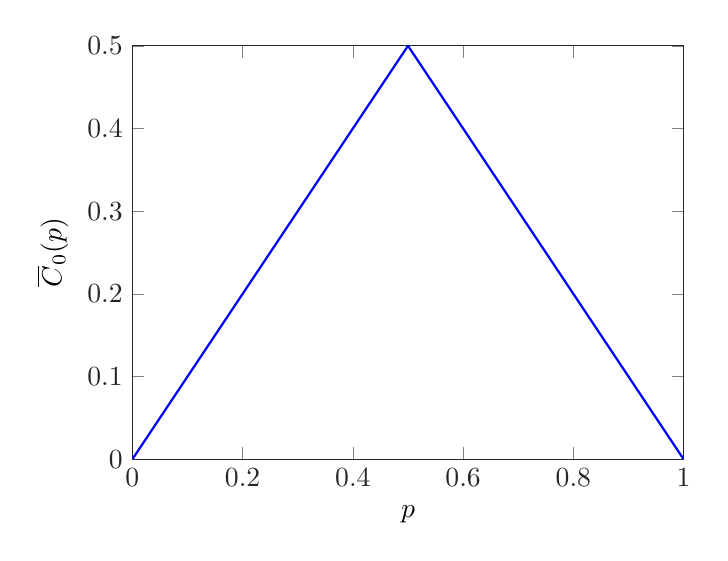
\begin{tikzpicture}
			\begin{axis}[%
				width=7cm,
				height=5.25cm,
				scale only axis,
				separate axis lines,
				every outer x axis line/.append style={white!15!black},
				every x tick label/.append style={font=\color{white!15!black}},
				xmin=0,
				xmax=1,
				xlabel={$p$},
				every outer y axis line/.append style={white!15!black},
				every y tick label/.append style={font=\color{white!15!black}},
				ymin=0,
				ymax=0.5,
				ylabel={$\overline{C}_0(p)$},
				legend style={draw=white!15!black,fill=white,legend cell align=left,legend pos=south east},
				]
				\addplot[blue,thick,domain=0:0.5,samples = 512] {x};
				\addplot[blue,thick,domain=0.5:1,samples = 512] {1 - x};
			\end{axis}
		\end{tikzpicture}
	\end{center}
	\caption{Minimum average cost with no observations}
	\label{fig:average_cost_n0}
\end{figure}

Let us now consider an arbitrary number of observations $n$, with $n >0$, and derive again the minimum expected cost detector, which minimizes the expected cost. This cost is denoted by $\overline{C}_n(p)$, to highlight that it depends on the number of observations and the prior probability $p$. Before proceeding, let us define $\mathbf{x}_n = (x[1], \ldots, x[n])^T$ as the vector that contains all available observations. Now, the sought detector is given by the likelihood ratio test (LRT), that is,
\begin{equation*}
	\frac{p_{{\bf X}_n|H}({\bf x}_n|1)}{p_{{\bf X}_n|H}({\bf x}_n|0)}\dunodcero \frac{c_{10}-c_{00}}{c_{01}-c_{11}} \frac{P_H(0)}{P_H(1)} = \frac{p}{1 - p}.
\end{equation*}
To compute the likelihood of the $n$ observations, we can use the i.i.d. assumption and, therefore,
\begin{equation*}
	p_{{\bf X}_n|H}({\bf x}_n|h) = \prod_{i = 1}^{n} p_{X[i]|H}( x[i] | h).
\end{equation*}
Using the likelihoods in \eqref{eq:likelihood_0} and \eqref{eq:likelihood_1}, we get
\begin{equation*}
	p_{{\bf X}_n|H}({\bf x}_n|0) = \prod_{i = 1}^{n} p_{X[i]|H}( x[i] | 0) = \prod_{i = 1}^{n} \frac{1}{\sqrt{2 \pi}} \exp \left(-\frac{x^2[i]}{2}\right) = \frac{1}{(2 \pi)^{n/2}} \exp \left(-\frac{1}{2} \sum_{i = 1}^{n} x^2[i]\right),
\end{equation*}
and
\begin{equation*}
	p_{{\bf X}_n|H}({\bf x}_n|1) = \prod_{i = 1}^{n} p_{X[i]|H}( x[i] | 1) = \prod_{i = 1}^{n} \frac{1}{\sqrt{8 \pi}} \exp \left(-\frac{x^2[i]}{8}\right) = \frac{1}{(8 \pi)^{n/2}} \exp \left(-\frac{1}{8} \sum_{i = 1}^{n} x^2[i]\right).
\end{equation*}
Then, the LRT becomes
\begin{equation*}
	\frac{\frac{1}{(8 \pi)^{n/2}} \exp \left(-\frac{1}{8} \sum_{i = 1}^{n} x^2[i]\right)}{\frac{1}{(2 \pi)^{n/2}} \exp \left(-\frac{1}{2} \sum_{i = 1}^{n} x^2[i]\right)} = \frac{1}{2^{n}} \exp \left(\frac{3 }{8} \sum_{i = 1}^{n} x^2[i]\right) \dunodcero \frac{p}{1 - p},
\end{equation*}
and the log-likelihood ratio test (LLRT) is
\begin{equation*}
  \frac{1}{n} \sum_{i = 1}^{n} x^2[i] \dunodcero \frac{8}{3} \left[\frac{1}{n} \log \left(\frac{p}{1 - p}  \right) + \log 2 \right].
\end{equation*}
Essentially, the LLRT compares the estimated variance with a threshold. The decision regions of the LLRT are
\begin{equation*}
	{\cal X}_1 = \left\{\x_n \in \mathbb{R}^{n} \left| \frac{1}{n} \sum_{i = 1}^{n} x^2[i]  >  \frac{8}{3} \left[ \frac{1}{n}  \log \left(\frac{p}{1 - p}  \right) + \log 2 \right] \right. \right\},
\end{equation*}
and
\begin{equation*}
	{\cal X}_0 = \left\{\x_n \in \mathbb{R}^{n} \left| \frac{1}{n} \sum_{i = 1}^{n} x^2[i]  \leq \frac{8}{3} \left[ \frac{1}{n}  \log \left(\frac{p}{1 - p}  \right) + \log 2 \right] \right. \right\}.
\end{equation*}
For these decision regions, we can compute the minimum expected cost as
\begin{align*}
	\overline{C}_n &= P(D = 1 | H = 0) p +  P(D = 0 |H = 1) (1 - p) \\
	&= p P_{\text{FA}} + (1 - p) P_{\text{M}},
\end{align*}
where
\begin{equation*}
	P_{\text{FA}} = P(D = 1 | H = 0) = \int_{{\cal X}_1} P_{{\bf X}_n|H}({\bf x}_n|0) d {\bf x}_n,
\end{equation*}
and
\begin{equation*}
	P_{\text{M}} = P(D = 0 | H = 1) = \int_{{\cal X}_0} P_{{\bf X}_n|H}({\bf x}_n|1) d {\bf x}_n.
\end{equation*}
Both, $P_{\text{FA}}$ and $P_{\text{M}}$, are given by complicated multidimensional integrals with no closed-form solution and that are difficult to evaluate numerically. Hence, we must compute them using a different approach.

We shall start by considering a transformation of the random variables $y[i], i = 1, \ldots, I$, which are Gaussian distributed with zero mean, unit variance, and i.i.d. Concretely, the transformation is
\begin{equation*}
	Z = \sum_{i = 1}^{I} y^2[i],
\end{equation*}
which is distributed as a Chi-squared random variable with $I$ degrees of freedom, denoted as $Z \sim \chi^2_{I}$. The probability density function of $Z$ is
\begin{equation*}
	p_Z(z) = \begin{cases} \frac{1}{2^{I/2} \Gamma(I/2)} z^{I/2 - 1} \exp(-z/2), & z >0, \\ 0, & \text{otherwise,} \end{cases}
\end{equation*}
and its cumulative distribution function is
\begin{equation*}
	F_Z(z) = \frac{\gamma(I/2,z/2)}{\Gamma(I/2)},
\end{equation*}
where $\Gamma(\cdot)$ is the gamma function and $\gamma(\cdot,\cdot)$ is the lower incomplete gamma function.\footnote{For positive integer values of the argument, the gamma function is given by $\Gamma(a) = (a - 1)!$. To compute the incomplete gamma function, it is necessary to resort to (uni-dimensional) numerical integration.} Figure \ref{fig:pdf_chi2} depicts $p_Z(z)$ and $F_Z(z)$ for a different number of degrees of freedom.

\begin{figure}[t]
	\begin{center}
		\includestandalone{Figures/Chi2_pdf} \includestandalone{Figures/Chi2_cdf}
	\end{center}
	\caption{Probability and cumulative density functions of a Chi-squared random variable with $I$ degrees of freedom}
	\label{fig:pdf_chi2}
\end{figure}

Using the Chi-squared distribution, we can compute $P_{\text{FA}}$ and $P_{\text{M}}$. The former is given by
\begin{align*}
	P_{\text{FA}} &= P(D = 1 | H = 0) \\ 
	&= P \left(\left. \frac{1}{n} \sum_{i = 1}^{n} x^2[i]  > \frac{8}{3} \left[ \frac{1}{n}  \log \left(\frac{p}{1 - p}  \right) + \log 2 \right] \right| H = 0 \right) \\ 
	&= P \left(\left. \sum_{i = 1}^{n} x^2[i]  > \frac{8}{3} \left[\log \left(\frac{p}{1 - p}  \right) + n \log 2 \right] \right| H = 0 \right),
\end{align*}
and taking into account that, under $H = 0$, $x[i]$ are i.i.d. Gaussian variables with zero mean and unit variance, $P_{\text{FA}}$ is the probability that a $\chi^2_n$ random variable is larger than $8/3 \left[\log \left(p/(1 - p)  \right) + n \log 2\right]$. That is,
\begin{equation*}
	P_{\text{FA}} = 1 - \frac{\gamma \left(n/2,\frac{8}{3} \left[\log \left(\frac{p}{1 - p}\right) + n \log 2 \right]\right)}{\Gamma(n/2)}.
\end{equation*}
We can proceed similarly for $P_{\text{M}}$ as follows
\begin{align*}
	P_{\text{M}} &= P(D = 0 | H = 1) \\ 
	&= P \left(\left. \frac{1}{n} \sum_{i = 1}^{n} x^2[i]  \leq \frac{8}{3} \left[ \frac{1}{n}  \log \left(\frac{p}{1 - p}  \right) + \log 2 \right] \right| H = 1 \right) \\ 
	&= P \left(\left. \sum_{i = 1}^{n} \left(\frac{x[i]}{2}\right)^2  \leq \frac{2}{3} \left[\log \left(\frac{p}{1 - p}  \right) + n \log 2 \right] \right| H = 1 \right).
\end{align*}
Under $H = 1$, $x[i]/2$ are i.i.d. Gaussian variables with zero mean and unit variance, and $P_{\text{M}}$ is therefore the probability that a $\chi^2_n$ random variable is smaller than $2/3 \left[\log \left(p/(1 - p)  \right) + n \log 2\right]$, which can be expressed as
\begin{equation*}
	P_{\text{M}} = \frac{\gamma \left(n/2,\frac{2}{3} \left[\log \left(\frac{p}{1 - p}  \right) + n \log 2 \right]\right)}{\Gamma(n/2)}.
\end{equation*}
\begin{figure}[t]
	\begin{center}
		\includestandalone{Figures/Expected_Cost1}
	\end{center}
	\caption{Minimum average cost with $n$ observations}
	\label{fig:average_cost_n}
\end{figure}
Hence, the expected cost becomes
\begin{multline}
	\overline{C}_n(p) = p \left(1 - \frac{\gamma \left(n/2,\frac{8}{3} \left[\log \left(\frac{p}{1 - p}  \right) + n \log 2 \right]\right)}{\Gamma(n/2)}\right) \\ + (1 - p) \left(\frac{\gamma \left(n/2,\frac{2}{3} \left[\log \left(\frac{p}{1 - p}  \right) + n \log 2 \right]\right)}{\Gamma(n/2)}\right), \label{eq:cost_n_nogathering}
\end{multline}
Let us now point out that the second argument of $\gamma \left(\cdot, \cdot\right)$ is negative for
\begin{align*}
%	8/3 \left[\log \left(\frac{p}{1 - p}  \right) + n \log 2\right] < 0 \nonumber \\
%	\log \left(\frac{p}{1 - p}  \right) + n \log 2 < 0  \nonumber \\
%	\log 2^n > \log \left(\frac{1 - p}{p}  \right) \nonumber \\
%	2^n < \frac{1 - p}{p}  \nonumber \\
%	p 2^n < 1 - p   \nonumber \\
%	p (2^n + 1) < 1 \nonumber \\
	p < \frac{1}{2^n + 1},
\end{align*}
making the lower incomplete gamma function zero, which yields
\begin{equation*}
	\overline{C}_n(p) = p,
\end{equation*}
for $p < \frac{1}{2^n + 1}$.

Figure \ref{fig:average_cost_n} shows $\overline{C}_n(p)$ for some values of $n$, which shows that
\begin{equation*}
	\overline{C}_0(p)  \geq \overline{C}_1(p) \geq \cdots \geq \overline{C}_n(p) \geq \cdots
\end{equation*}
Then, we should keep acquiring samples as long as we can (larger $n$) and, as a consequence, get a smaller minimum average cost.

\subsection{Example 2: Sequential detection with gathering cost}

\begin{figure}[t]
	\begin{center}
		\includestandalone{Figures/Expected_Cost2}
	\end{center}
	\caption{Minimum average cost, including the gathering cost, with $n$ observations}
	\label{fig:average_cost2_n}
\end{figure}

The results of the previous example do not make a lot of sense as we should keep collecting samples forever if we are to minimize the minimum average cost. Actually, for $n \rightarrow \infty$ we have $\overline{C}_n(p) \rightarrow 0$, regardless of $p$. Intuitively, we should include a cost every time an observation is collected, which should include a gathering cost related to, i.e., power consumption of the acquisition and transmission devices, and a waiting cost. Let us go back to the previous example and repeat it considering that this gathering (and waiting) cost is $c_{G} = 0.05$.

Taking into account $c_{G}$ and $\overline{C}_n(p)$ derived in \eqref{eq:cost_n_nogathering}, the modified cost is given by
\begin{multline*}
	\overline{C}_{n,G}(p)  = p \left(1 - \frac{\gamma \left(n/2,\frac{8}{3} \left[\log \left(\frac{p}{1 - p}  \right) + n \log 2 \right]\right)}{\Gamma(n/2)}\right) \\ + (1 - p) \left(\frac{\gamma \left(n/2,\frac{2}{3} \left[\log \left(\frac{p}{1 - p}  \right) + n \log 2 \right]\right)}{\Gamma(n/2)}\right) + c_G \cdot n,
\end{multline*}
which is depicted in Figure \ref{fig:average_cost2_n}. From this figure, we can notice that keeping collecting samples does not necessarily improve $\overline{C}_{n,G}(p)$ as it happened in the case of no gathering cost, that is, $\overline{C}_{n,G}(p) \not \geq \overline{C}_{n+1,G}(p), \forall p \in [0,1]$. However, there is a range of values of $p$, for which it holds that $\overline{C}_{n,G}(p) \geq \overline{C}_{n+1,G}(p)$. Hence, sometimes it will be convenient to acquire an additional samples and sometimes it will not. Precisely this idea is the main ingredient of sequential detection.

\section{Sequential test}

We have used the previous examples to motivate sequential detection, but such story is not completely accurate because to derive the minimum expected cost at time $n$, the detector needs to use $n$ samples. However, we need to make the decision every time a new sample is acquired, which makes the story a bit simpler as we shall see.
 % what happens if  we had stopped earlier or what happens to the gathering cost of the previous time instants once we have already acquired those observations. In fact, the story is a bit simpler.

\begin{figure}[t]
	\begin{center}
		\includestandalone{Figures/Expected_Cost3}
	\end{center}
	\caption{Minimum average cost, including the gathering cost, with $n$ observations}
	\label{fig:average_cost3_n}
\end{figure}

Consider there are no observations available, that is $n = 0$. At this time instant, we need to decide between $H = 0$, $H = 1$, or take another sample. Since there are no available samples, the cost of always deciding $D = 1$ is $p$, the prior probability of $H = 0$, the cost of always deciding $D = 0$ is $1 - p$, the prior probability of $H = 1$, and the minimum expected cost with $n = 1$ sample is $\overline{C}_{1,G}(p)$. These three costs are depicted in Figure \ref{fig:average_cost3_n}, which shows that they intersect at two points. The first of these two points, $p_L$, can be obtained as the largest value of $p$ for which $\overline{C}_{1,G}(p)$ is still larger than the cost of always deciding $D = 1$. Mathematically, $p_L$ is obtained as
\begin{equation*}
	p_L = \sup_{p} \ \{p \mid \overline{C}_{1,G}(p) > p\}.
\end{equation*}
Similarly, $p_U$ is the smallest value of $p$ where $\overline{C}_{1,G}(p)$ starts to be larger than the cost of always deciding $D = 0$, that is,
\begin{equation*}
	p_U = \inf_{p} \  \{p \mid \overline{C}_{1,G}(p) > 1 - p\}.
\end{equation*}
Hence, for $p \in [0,p_L]$, with $p_L = 0.4057$ in our example, the cost of always deciding $D = 1$ is the smallest, whereas for $p \in [p_U,1]$, with $p_U = 0.7403$, the cost of always deciding $D = 0$ is the smallest. However, for $p \in (p_L,p_U)$, neither the cost of always deciding $D = 0$, nor the cost of always deciding $D = 1$ is the smallest, and we must take another sample. Summarizing, at time $n = 0$, the sequential test must\footnote{Although this sequential test was obtained for a particular example, it is a general result since $\overline{C}_{1,G}(p)$ is a concave function of $p$ in $[0,1]$ for any likelihood and any other costs $c_{DH}$ and $c_{G}$. Nevertheless, the derived values of $p_L$ and $p_U$ would be different.}
\begin{equation}
\label{eq:seq_test_n0}
\begin{array}{l}
	\text{decide } D = 1 \text{ for } p \leq p_L, \\
	\text{decide } D = 0 \text{ for } p \geq p_U, \\
	\text{take another sample for } p_L < p < p_U.
\end{array}
\end{equation}

The question that remains to be answered is: What do we have to do if we have decided to take another sample? To answer this question, we must note that at $n = 1$, we have already taken the sample, i.e., the gathering cost has been already spent. Moreover, the possible decisions at $n = 1$ are exactly those of $n = 0$: decide between $H = 0$, $H = 1$, or take another sample. That is, the effect of having already taken one sample does not modify the test as there are still an infinite number of available samples. However, there is one important difference. The value of $x[1]$ provides some (partial) knowledge about the hypothesis. Then, conditioned on having observed $x[1]$, we should repeat the sequential test in \eqref{eq:seq_test_n0}, but instead of using the prior probability $P(H = 0) = p$, we must use the posterior probability $P(H = 0 | X[1] = x[1]) = p_1$, i.e.,
\begin{equation*}
	\begin{array}{l}
		\text{decide } D = 1 \text{ for } p_1 \leq p_L, \\
		\text{decide } D = 0 \text{ for } p_1 \geq p_U, \\
		\text{take another sample for } p_L < p < p_U.
	\end{array}
\end{equation*}
Similarly, at a generic time $n$, the sequential test is
\begin{equation}
	\label{eq:seq_test}
	\begin{array}{l}
		\text{decide } D = 1 \text{ for } p_n \leq p_L, \\
		\text{decide } D = 0 \text{ for } p_n \geq p_U, \\
		\text{take another sample for } p_L < p < p_U,
	\end{array}
\end{equation}
where the posterior probability is now
\begin{equation*}
	p_n = P(H = 0 | X[1] = x[1], \ldots, X[n] = x[n]),
\end{equation*}
with $p_0 = P(H = 0) = p$. To conclude the derivation of the sequential test, we must find an explicit expression for $p_n$. First, using Bayes's theorem we can rewrite $p_n$ as
\begin{align*}
	p_n &= P(H = 0 | X[1] = x[1], \ldots, X[n] = x[n]) \\ &= \frac{P(H = 0 , X[1] = x[1], \ldots, X[n] = x[n])}{P(X[1] = x[1], \ldots, X[n] = x[n])} \\ &= \frac{P(X[1] = x[1], \ldots, X[n] = x[n] | H = 0) P_H(0)}{P(X[1] = x[1], \ldots, X[n] = x[n])}.
\end{align*}
Applying now the law of total probability to the denominator, $p_n$ becomes
\begin{align}
	p_n &= \frac{P(X[1] = x[1], \ldots, X[n] = x[n] | H = 0) P(H = 0)}{\displaystyle \sum_{h = 0}^{1} P(X[1] = x[1], \ldots, X[n] = x[n] | H = h) P_H(h)} \nonumber \\ &= 
	\frac{p_{\mathbf{X}_n | H}(\x_n | 0) p}{p_{\mathbf{X}_n | H}(\x_n | 0) p + p_{\mathbf{X}_n | H}(\x_n | 1) (1 - p)}, \label{eq:pn_pre}
\end{align}
which is a function of both likelihoods, $P_{\mathbf{X}_n | H}(\x_n | 0)$ and $P_{\mathbf{X}_n | H}(\x_n | 1)$, and $p$. Finally, taking into account the i.i.d. assumption, we can simplify \eqref{eq:pn_pre} as
\begin{equation}
	\label{eq:pn}
	p_n = \frac{p}{\displaystyle p +  (1 - p) \frac{p_{\mathbf{X}_n | H}(\x_n | 1)}{p_{\mathbf{X}_n | H}(\x_n | 0)}} = \frac{p}{\displaystyle p +  (1 - p) \prod_{i = 1}^{n} \frac{p_{X[i] | H}(x[i] | 1)}{p_{X[i] | H}(x[i] | 0)}},
\end{equation}
where, for the sake of consistency, we define $\prod_{i = 1}^{0} = 1$.

Finally, and continuing with our example, where
\begin{equation*}
	\frac{p_{X[i] | H}(x[i] | 1)}{p_{X[i] | H}(x[i] | 0)} = \frac{1}{2} \exp \left(\frac{3 }{8} x^2[i] \right), \ i = 1, 2, \ldots,
\end{equation*}
Figure \ref{fig:seq_test_realizations} shows several realizations of the sequential test in \eqref{eq:seq_test} for this example, when $p = 0.5$. Some of these realizations were obtained for $x[n]$ generated under $H = 0$ and other realizations for  $x[n]$ generated under $H = 1$. In this figure, we can see that as soon as $p_n$ is above $p_U$ or below $p_L$, the detector stops the acquisition of more observations. In the former case, the decision is $D = 0$, whereas in the latter, it is $D = 1$.
\begin{figure}[t]
	\begin{center}
		\includestandalone{Figures/seq_test_realizations}
	\end{center}
	\caption{Realizations of the sequential test}
	\label{fig:seq_test_realizations}
\end{figure}

\section{Sequential probability ratio test}

Using \eqref{eq:pn}, the sequential test in \eqref{eq:seq_test} is
\begin{equation}
	\label{eq:seq_SPRT_mincost}
	\begin{array}{l}
		\text{decide } D = 1 \text{ for } \phi_n \geq \frac{p (1 - p_L)}{p_L(1 - p)}, \\
		\text{decide } D = 0 \text{ for } \phi_n \leq  \frac{p (1 - p_U)}{p_U (1 - p)}, \\
		\text{take another sample for } \frac{p (1 - p_U)}{p_U (1 - p)} < \phi_n < \frac{p (1 - p_L)}{p_L(1 - p)},
	\end{array}
\end{equation}
where
\begin{equation*}
	\phi_n = \prod_{i = 1}^{n} \frac{p_{X[i] | H}(x[i] | 1)}{p_{X[i] | H}(x[i] | 0)}.
\end{equation*}
% \begin{align}
%	 \eta_U &= \frac{p (1 - p_L)}{p_L(1 - p)},  & \eta_L &= \frac{p (1 - p_U)}{p_U (1 - p)}. \label{eq:eta_mincost}
%\end{align}
Then, the sequential test boils down to a likelihood ratio test, and it is therefore named the sequential probability ratio test (SPRT). Note that the SPRT can be computed recursively when a new observation comes in, i.e.,
\begin{equation*}
	\phi_n = \prod_{i = 1}^{n} \frac{P_{X[i] | H}(x[i] | 1)}{P_{X[i] | H}(x[i] | 0)} = \left(\prod_{i = 1}^{n-1} \frac{P_{X[i] | H}(x[i] | 1)}{P_{X[i] | H}(x[i] | 0)}\right) \frac{P_{X[n] | H}(x[n] | 1)}{P_{X[n] | H}(x[n] | 0)} = \phi_{n-1} \cdot \frac{P_{X[n] | H}(x[n] | 1)}{P_{X[n] | H}(x[n] | 0)},
\end{equation*}
with $\phi_0 = 1$.

Actually, \eqref{eq:seq_SPRT_mincost} is just one example of the SPRT for a particular choice of the thresholds (those that optimize the expected cost). The most general SPRT is given by
\begin{equation}
	\label{eq:seq_SPRT}
	\begin{array}{l}
		\text{decide } D = 1 \text{ for } \phi_n \geq \eta_U, \\
		\text{decide } D = 0 \text{ for } \phi_n \leq  \eta_L, \\
		\text{take another sample for } \eta_L < \phi_n < \eta_U,
	\end{array}
\end{equation}
where the thresholds should satisfy
\begin{equation*}
	0 < \eta_L < 1 < \eta_U < \infty.
\end{equation*}
Intuitively, for larger values of $\eta_U$, it is more unlikely to decide $D = 1$. This implies that it will take longer to decide $D = 1$, while at the same time, it will be more unlikely to decide $D = 1$ when $H = 0$. Similarly, for smaller values of $\eta_L$, it is more unlikely to decide $D = 0$ and, therefore, it will take longer to decide $D = 0$, while at the same time, it will be more unlikely to decide $D = 0$ when $H = 1$. These suggests that there are three metrics at play: the probability of false alarm ($\pfa = P(D = 1 | H = 0)$), the probability of missing ($\pmis = P(D = 0 | H = 1)$), and the sample size $N$, which is defined as
\begin{equation*}
	\label{eq:sample_size}
	N =  \min_{n} \ \{n \mid \phi_n \geq \eta_U \text{ or } \phi_n \leq \eta_L\}. 
\end{equation*}
Thus,  the most established objective is to design the SPRT, i.e., the thresholds $\eta_L$ and $\eta_U$ in \eqref{eq:seq_SPRT}, that minimizes $N$ while guaranteeing that $\pfa \leq \alpha$ and $\pmis \leq \beta$, where $\alpha$ and $\beta$ are the target values of probability of false alarm and probability of missing, respectively. In the following, we will derive $\pfa$ and $\pmis$ as a function of the thresholds.

Let us start by the probability of false alarm, which is defined as
\begin{equation*}
	\pfa = P(D = 1 | H = 0) = \int_{\mathcal{X}_1} p_{\mathbf{X}_{\infty} | H} (\mathbf{x}_{\infty} | 0) d \mathbf{x}_{\infty},
\end{equation*}
where $\mathbf{x}_{\infty} \in \mathbb{R}^{\infty}$ and
\begin{equation*}
	\mathcal{X}_1 = \{ \mathbf{x}_{\infty} \in \mathbb{R}^{\infty} | \phi_{N} \geq  \eta_U  \}.
\end{equation*}
To continue, we must note that the set $\mathcal{X}_1$ can be decomposed as
\begin{equation*}
	\mathcal{X}_1 = \mathop{\bigcup}\limits_{n = 1}^{\infty} \mathcal{X}_{1,n},
\end{equation*}
with
\begin{equation*}
	\mathcal{X}_{1,n} = \{ \mathbf{x}_{\infty} \in \mathbb{R}^{\infty} |N = n \text{ and } \phi_{n} \geq  \eta_U  \}.
\end{equation*}
That is, we decide $D = 1$ when we decide $D = 1$ at $n = 1$, or at $n = 2$, or at $n = 3$, $\ldots$ Moreover, taking into account that if we decide $D = 1$ at $n$, we could not decide it at a different time instant $m$, with $n \neq m$, the sets $\mathcal{X}_{1,n}$ and $\mathcal{X}_{1,m}$ are mutually exclusive, i.e., they do not overlap, allowing us to write
\begin{align*}
	\pfa &= \int_{\mathcal{X}_1} p_{\mathbf{X}_{\infty} | H} (\mathbf{x}_{\infty} | 0) d \mathbf{x}_{\infty} 
	= \int_{\cup_{n = 1}^{\infty} \mathcal{X}_{1,n}} p_{\mathbf{X}_{\infty} | H} (\mathbf{x}_{\infty} | 0) d \mathbf{x}_{\infty} 
	= \sum_{n = 1}^{\infty}  \int_{\mathcal{X}_{1,n}} p_{\mathbf{X}_{n} | H} (\mathbf{x}_{n} | 0) d \mathbf{x}_{n} \\
	&= \sum_{n = 1}^{\infty}  \int_{\mathcal{X}_{1,n}} \prod_{i = 1}^{n} p_{X[i] | H}(x[i] | 0)  d \mathbf{x}_{n}.
\end{align*}
Using now that
\begin{equation*}
	\phi_n \geq \eta_U \Rightarrow   \prod_{i = 1}^{n} p_{X[i] | H}(x[i] | 0) \leq \eta_U^{-1} \prod_{i = 1}^{n} p_{X[i] | H}(x[i] | 1)
\end{equation*}
for $\mathbf{x}_n \in \mathcal{X}_{1,n}$, we have 
\begin{equation*}
	\pfa \leq  \eta_U^{-1} \sum_{n = 1}^{\infty}  \int_{\mathcal{X}_{1,n}}  \prod_{i = 1}^{n} p_{X[i] | H}(x[i] | 1)  d \mathbf{x}_{n}.
\end{equation*}
Since the probability of detection is
\begin{align*}
	\pdet &= \int_{\mathcal{X}_1} p_{\mathbf{X}_{\infty} | H} (\mathbf{x}_{\infty} | 1) d \mathbf{x}_{\infty} 
	= \sum_{n = 1}^{\infty}  \int_{\mathcal{X}_{1,n}} \prod_{i = 1}^{n} p_{X[i] | H}(x[i] | 1)  d \mathbf{x}_{n} \\
	&= 1 - \pmis,
\end{align*}
we get
\begin{equation}
	\label{eq:bound_pfa}
	\pfa \leq  \eta_U^{-1} \left(1 - \pmis\right).
\end{equation}

To compute the probability of missing, it is possible to follow a similar approach. Define
\begin{equation*}
	\mathcal{X}_0 = \{ \mathbf{x}_{\infty} \in \mathbb{R}^{\infty} | \phi_{N} \leq  \eta_L  \} = \mathop{\bigcup}\limits_{n = 1}^{\infty} \mathcal{X}_{0,n},
\end{equation*}
where
\begin{equation*}
	\mathcal{X}_{0,n} = \{ \mathbf{x}_{\infty} \in \mathbb{R}^{\infty} |N = n \text{ and } \phi_{n} \leq  \eta_L  \}.
\end{equation*}
Hence, the probability of missing is
\begin{equation*}
	\pmis = P(D = 0 | H = 1) = \int_{\mathcal{X}_0} p_{\mathbf{X}_{\infty} | H} (\mathbf{x}_{\infty} | 1) d \mathbf{x}_{\infty} = \sum_{n = 1}^{\infty}  \int_{\mathcal{X}_{0,n}} \prod_{i = 1}^{n} p_{X[i] | H}(x[i] | 1)  d \mathbf{x}_{n}.
\end{equation*}
The above expression can be bounded as
\begin{equation*}
	\pmis \leq  \eta_L \sum_{n = 1}^{\infty}  \int_{\mathcal{X}_{0,n}}  \prod_{i = 1}^{n} p_{X[i] | H}(x[i] | 0)  d \mathbf{x}_{n},
\end{equation*}
since
\begin{equation*}
	\phi_n \leq \eta_L \Rightarrow   \prod_{i = 1}^{n} p_{X[i] | H}(x[i] | 1) \leq \eta_L \prod_{i = 1}^{n} p_{X[i] | H}(x[i] | 0),
\end{equation*}
for $\mathbf{x}_n \in \mathcal{X}_{0,n}$. Finally, we get
\begin{equation}
	\label{eq:bound_pm}
	\pmis \leq  \eta_L (1 - \pfa),
\end{equation}
where we have taken into account that
\begin{equation*}
	\sum_{n = 1}^{\infty}  \int_{\mathcal{X}_{0,n}}  \prod_{i = 1}^{n} p_{X[i] | H}(x[i] | 0)  d \mathbf{x}_{n} = 1 - \sum_{n = 1}^{\infty}  \int_{\mathcal{X}_{1,n}}  \prod_{i = 1}^{n} p_{X[i] | H}(x[i] | 0)  d \mathbf{x}_{n} = 1 - \pfa.
\end{equation*}

The bounds for the probabilities of false alarm and missing in \eqref{eq:bound_pfa} and \eqref{eq:bound_pm} allow us to obtain the values $\eta_L$ and $\eta_U$ that achieve the desired value for $P_{\text{FA}}$ and $P_{\text{M}}$. Concretely, we only need to solve the inequalities in \eqref{eq:bound_pfa} and \eqref{eq:bound_pm}, which yields
\begin{align*}
	\eta_L &\geq \frac{\pmis}{1 - \pfa},  &  \eta_U &\leq  \frac{1 - \pmis}{\pfa},
\end{align*}
which are, in fact, only bounds. To avoid the inequalities and derive (approximate) equalities, we need to assume that when $\phi_N$ crosses the boundaries $\eta_L$ and $\eta_U$, the excess over the boundaries is negligible. That is,
\begin{align*}
	\phi_N - \eta_U &\rightarrow \epsilon_1,  &  \eta_L - \phi_N &\rightarrow \epsilon_2,
\end{align*}
with $\epsilon_i$ arbitrarily small positive constants. Under these assumptions, which are very accurate for large $N$, we get 
\begin{align*}
	\eta_L &\approx \frac{\pmis}{1 - \pfa},  &  \eta_U &\approx  \frac{1 - \pmis}{\pfa},
\end{align*}
which are known as Wald's approximations. Interestingly, and contrary to what happens with the LRT, the thresholds required to achieve the desired probabilities of false alarm and missing do not depend on the likelihoods. Nevertheless, the SPRT does depend on the likelihoods, and so do the sample size, $N$, and the expected sample size, $\mathbb{E}\{N\}$.

We conclude the topic of sequential detection by presenting the Wald-Wolfowitz theorem. Let us denote the probabilities of false alarm and missing of the SPRT $\pfa(\phi)$ and $\pmis(\phi)$, and its sample size $N(\phi)$. Consider an alternative sequential decision rule with probabilities of false alarm and missing $\pfa(\psi)$ and $\pmis(\psi)$, which satisfy
\begin{align*}
	\pfa(\psi) &\leq \pfa(\phi), & \pmis(\psi) &\leq \pmis(\phi).
\end{align*}
Then, the Wald-Wolfowitz theorem states that
\begin{equation*}
	\mathbb{E} \{N(\psi)\} \geq \mathbb{E} \{N(\phi)\},
\end{equation*}
where $N(\psi)$ is the sample size of the alternative decision rule. Hence, for a desired level of performance ($\pfa \leq \alpha$ and $\pmis \leq \beta$), there does not exist any sequential decision rule that achieves an expected sample size smaller than that of the SPRT. Interestingly, since a fixed-sample-size detector can be seen as a (very particular) sequential decision rule, the average sample size of the SPRT can not be larger than the sample size of any fixed-sample-size detector  with the same level of performance. Alternatively, the Wald-Wolfowitz theorem also states that, for a fixed expected sample size, there is no sequential rule that achieves smaller $\pfa$ and $\pmis$ than those of the SPRT.


% Appendix
%%%%%%%%%%%%%%%%%%%%% appendix.tex %%%%%%%%%%%%%%%%%%%%%%%%%%%%%%%%%
%
% sample appendix
%
% Use this file as a template for your own input.
%
%%%%%%%%%%%%%%%%%%%%%%%% Springer-Verlag %%%%%%%%%%%%%%%%%%%%%%%%%%

\appendix
%\motto{All's well that ends well}
\chapter{Transformations of random variables}
\label{introA} % Always give a unique label
% use \chaptermark{}
% to alter or adjust the chapter heading in the running head

%%%%%%%%%%%%%%%%%%%%%%%%%%%%%%%%%%%
\section{Change of Random Variable}
\label{sec:1}
%%%%%%%%%%%%%%%%%%%%%%%%%%%%%%%%%%%

Let's consider we know the probability of a r.v. $X$, $\px$, and we now want to compute the probability density function of some variable $Y=f(X)$, that is, we need to calculate $\py$.

To understand how this new distribution or {\bf change of random variable} is calculated, let's firstly solve a particular case:

\begin{itemize}
\item $X$ is a uniform distribution in the interval $(0,1)$.

\begin{center}
\begin{tabular}{m{.5\textwidth}m{.4\textwidth}}
 \begin{equation} 
\px = \begin{cases}
1 & {\rm if} \quad 0<x<1\\
0 & {\rm otherwise} 
\end{cases} \nonumber
\end{equation} & 
\raisebox{-8ex}{\includegraphics[scale=.25]{Figures/Fig11.png}} \\ 
\end{tabular}
\end{center}

\item $Y = X^2$. Note that this change produces this transformation:
\begin{center}
\begin{tabular}{m{.5\textwidth}m{.4\textwidth}}
 \raisebox{-8ex}{\includegraphics[scale=.4]{Figures/Fig12.png}} &
 \begin{tabular}{l|l}
$x$ & $y = x^2$ \\ \hline
0.1 & 0.01\\
0.2 & 0.04\\
0.5 & 0.25\\
... & ...\\
\end{tabular} 
\end{tabular}
\end{center}

The transformation function $f(\cdot)$ is strictly increasing. So there exists its inverse function $f^{-1}(\cdot)$.

\end{itemize}
To solve this change of r.v., we are going to use the fact that:

\begin{eqnarray}
P\{0<X<0.1\} &  = & P\{0<Y<0.01\}  \nonumber\\
P\{0<X<0.2\} &  = & P\{0<Y<0.04\}  \nonumber\\
P\{0<X<0.5\} &  = & P\{0<Y<0.25\}  \nonumber
\end{eqnarray}
or, in a general case, for any value of $X$, $x_0$, we have
$$ P\{0<X<x_0\}  = P\{0<Y<y_0\}$$
where $y_0=x_0^2$ or $x_0= \sqrt{y_0}$ 

So, we can compute the cumulative distribution function of the r.v. $Y$ as
$$ F_Y(y_0) =  P\{Y<y_0\} =  P\{X<\sqrt{y_0}\}$$

Now, as the cumulative function of $Y$ is expressed in terms of the r.v $X$, we can compute it!!!
\begin{eqnarray} 
F_Y(y_0) =  P\{X<\sqrt{y_0}\} = \int_{-\infty}^{\sqrt{y_0}} \px dx = 
\begin{cases}
\int_{-\infty}^{\sqrt{y_0}} 0 dx = 0 & \quad {\rm if} \quad y_0 <0 \\[2ex]
\int_0^{\sqrt{y_0}} 1 dx = \sqrt{y_0} & \quad {\rm if} \quad 0< y_0 <1 \\[2ex]
\int_0^{1} 1 dx = 1 & \quad {\rm if} \quad y_0 >1 \\
\end{cases}  \nonumber
\end{eqnarray}

So, we have that
\begin{eqnarray} 
F_Y(y_0) =\begin{cases}
 0 & \quad {\rm if} \quad y_0 <0 \\
 \sqrt{y_0} & \quad {\rm if} \quad 0< y_0 <1 \\
 1 & \quad {\rm if} \quad y_0 >1 \\
\end{cases}  \nonumber
\end{eqnarray} 
\begin{center}
\includegraphics[scale=.4]{Figures/Fig13.png}
\end{center}
and, finally, we can obtain the density function of $Y$ as
\begin{eqnarray} 
\py = \frac{d F_Y(y)}{dy} =\begin{cases}
 \frac{1}{2\sqrt{y}} & \quad {\rm if} \quad 0<y<1 \\
 0 & \quad {\rm otherwise}  \\
\end{cases}  \nonumber
\end{eqnarray} 
\begin{center}
\includegraphics[scale=.4]{Figures/Fig14.png}
\end{center}
Now, let's try to generalize this procedure for any transformation
$$ Y = f(X) $$
being $f(\cdot)$ a strictly increasing function, so $f^{-1}(\cdot)$ exists.
\begin{enumerate}
    \item Compute the cumulative function of $Y$ (by means of $X$)
    \begin{eqnarray} 
    F_Y(y)  &= &  P\{Y<y\} =  P\{X<f^{-1}(y)\} = \int_{-\infty}^{f^{-1}(y)} \px dx = \nonumber \\ 
    & & F_X(f^{-1}(y)) - F_X(-\infty) = F_X(f^{-1}(y)) \nonumber
    \end{eqnarray} 
  Note: $F_X(-\infty) = 0$ for any cumulative distribution function  
    \item Compute the density distribution function (use the chain rule)
    \begin{eqnarray} 
    \py = \frac{d F_Y(y)}{dy} =  \frac{d F_X(f^{-1}(y))}{dy} = \frac{d F_X(x= f^{-1}(y))}{dx}  \frac{dx}{dy} = p_X(x= f^{-1}(y)) \frac{dx}{dy} \nonumber
    \end{eqnarray} 
    So, we obtain that 
    \begin{eqnarray}  \py = p_X(x= f^{-1}(y)) \frac{dx}{dy}  \nonumber \end{eqnarray} 
\end{enumerate}

This formula for the r.v. change can be generalized for any transformation function $f(\cdot)$ which is monotic (either strictly increasing or decreasing) as follows:
\begin{svgraybox}
\begin{equation} 
\py = p_X(x = f^{-1}(y))  \left| \frac{dx}{dy}\right| \label{eq:changeRV}
\end{equation} 
\end{svgraybox}

In fact, we can now use this formula over the previous example:
\begin{center}
\begin{tabular}{m{.2\textwidth}m{.5\textwidth}}
 \raisebox{-0.25ex}{$ Y = X^2$} &
 \begin{equation} 
\px = \begin{cases}
1 & {\rm if} \quad 0<x<1\\
0 & {\rm otherwise} 
\end{cases} \nonumber
\end{equation}
\end{tabular}
\end{center}
each term of the formula \eqref{eq:changeRV} is given by:
\begin{eqnarray} 
\left| \frac{dx}{dy}\right| = \left| \frac{df^{-1}(y)}{dy}\right| = \left| \frac{d\sqrt{y}}{dy}\right| = \frac{1}{2\sqrt{y}} \nonumber
\end{eqnarray} 

\begin{eqnarray} 
p_X(x = f^{-1}(y)) = p_X(x = \sqrt{y}) = \begin{cases}
1 & {\rm if} \quad 0<\sqrt{y}<1\\
0 & {\rm otherwise} 
\end{cases}  \nonumber
\end{eqnarray} 

So, we get

\begin{eqnarray} 
\py  = \frac{1}{2\sqrt{y}} p_X(x = \sqrt{y}) = \begin{cases}
\frac{1}{2\sqrt{y}} & {\rm if} \quad 0<y<1\\
0 & {\rm otherwise} 
\end{cases}  \nonumber
\end{eqnarray} 

In case the transformation function is not monotic, we have to divide the transformation into intervals where we get monotic transformations. That is, we have $Y = f(X)$ and $f(\cdot)$ is not monotic, then redefine the transformation as
\begin{eqnarray} 
Y = \begin{cases} 
f_1(X) & {\rm if } x_0 < x <x_1 \\
f_2(X) & {\rm if } x_1 < x <x_2 \\
\ldots  &  \\
f_N(X) & {\rm if } x_{N-1} < x <x_N \\
\end{cases}  \nonumber
\end{eqnarray}

where $f_1(\cdot),\ldots, f_N(\cdot) $ are monotic. Then, you can compute $\py$ as:
\begin{eqnarray} 
\py =  \sum_{n=1}^N p_X(x = f_n^{-1}(y))  \left| \frac{df_n^{-1}(y)}{dy}\right| \nonumber
\end{eqnarray} 

%%%%%%%%%%%%%%%%%%%%%%%%%%%%%%%%%%%%
\subsection{Some usual r.v. changes}

The demonstration of these changes is left as homework.

\begin{enumerate}
    \item SHIFTING of R.V. \\
    $ Y = X+a$, where $a$ is a known constant. Then,
    $$ \py =  p_X(x = y-a) $$
    when we are adding a constant to any r.v., we are shifting the distribution from the origin to the position of the constant
    
    \begin{center}
    \includegraphics[scale=.3]{Figures/Fig15.png}
    \end{center}
    
    
    \item RESCALING of R.V.\\
    $ Y = aX$, where $a$ is a known constant. Then,
    $$ \py =  \frac{1}{a} p_X(x = \frac{y}{a}) $$
    in this case we are modifying both the support of the distribution function and its height.
    
    \begin{center}
    \includegraphics[scale=.3]{Figures/Fig16.png}
    \end{center}
    
\end{enumerate}

%\include{Contents/probability/chapter1}

%%%%%%%%%%%%%%%%%%%%%%%%%%%%%%%
\chapter{Introductory examples}
\label{introB}
\section{Some introductory examples}
\label{sec:M2}

The contents of this section provide an introduction to the detection problem in the binary case using some simple examples. Concretely, we will present some basic concepts through these examples. Important concepts, such as hypothesis, their {\em a priori} and {\em a posteriori} probabilities, likelihoods, or cost and cost function, will be introduced.

Before proceeding, we would like to point out that detection theory is the term employed by some communities, while some use hypothesis testing and others classification.

\subsection{Example 1: Binary detection with no observations}
\label{subsec:example1}

\begin{problem}
Consider a game in which two dice are rolled and our task consists in deciding whether the sum of both dice is larger than or equal to 10, or smaller thereof. For this problem, you have to answer the following questions:
    \begin{itemize}
        \item[a)] What decision results in fewer errors in the long term?
        \item[b)] Consider now that not all errors are penalized the same. In particular, let us assume that the errors of wrongly deciding that the sum of the dice is larger than or equal to 10 ($S\geq 10$) are assigned a penalty (or cost) of $c$, whereas wrongly deciding $S<10$ results in a unit cost (per wrong guess). What would be in this case the long term cost of both decision strategies?
        \item[c)] What is the optimal strategy to minimize the expected cost? Provide your answer as a function of $c$.
    \end{itemize}
\end{problem}

\begin{solution}
Let us start by introducing some notation for this problem. Note that the design of a detector must always be done according to a criterion ``in the long term''. In other words, the goal is to analyze the average performance as the number of experiments tends to infinity. Hence, there are certain variables that will take different values in each experiment, and these need to be modeled by random variables.

    \begin{itemize}
    \item We denote by $X_1$ and $X_2$ the random variables (r.v.) that represent the result of each die roll. Since we consider fair dice, we have $P_{X_i}(x_i) = \frac{1}{6}$, for $i=1,2$, and for $x_i \in \{1, 2, 3, 4, 5, 6\}$.
    \item The sum of the dice is represented with the random variable $S = X_1 + X_2$.
    \item Finally, this problem involves two different hypotheses depending on the value of $S$. Since the true hypothesis can change between experiments, we introduce a discrete random variable $H$ that can take just two values
    \begin{align}
    h=0 & \text{~if and only if } \{s<10\} \nonumber \\
    h=1 & \text{~if and only if } \{s\geq10\} \nonumber
    \end{align}
    Note that, being a function of another random variable, $H$ is also a random variable, and it should be possible to compute its distribution from the distribution of $S$, which in turn can be calculated from the distributions of $X_1$ and $X_2$. Moreover, in this problem, there exists a causal relation between random variables, which implies that the hypotheses depend on $X_1$ and $X_2$. This has certain impact on how we can calculate statistical information, as we will discuss later.

    \end{itemize}
    
% In this course, we focus just on {\em hypothesis testing} problems, i.e., the goal is to decide among a set of possible hypotheses. Not all problems are of this type, but many interesting classification problems can be formulated in this way.

\begin{itemize}
    \item [a)] We first need to discuss what are the possible decisions that can be implemented. Building a detection system translates into designing a function that takes all available information as input, and outputs the selected hypothesis. Since we only consider deterministic functions, and in this case there are no input features, this implies that only two functions can be considered:
    \begin{itemize}
        \item A detector (function) that selects all the time hypothesis 0 (i.e., $d=0$).
        \item A detector (function) that selects all the time hypothesis 1 (i.e., $d=1$).
    \end{itemize}
    
    The probability of error of these two classifiers can be calculated as follows:
    \begin{itemize}
        \item For the former, $d=0$:
        $$P_e = P(H\neq d) = P(H \neq 0) = P_H(1).$$
        \item For the latter, $d=1$:
        $$P_e = P(H\neq d) = P(H \neq 1) = P_H(0).$$
    \end{itemize}

    Therefore, we need to compute the distribution of the r.v. $H$. To do so, we begin by calculating the probability distribution of $S$. Figure \ref{fig:dice} shows all possible outcomes of $X_1$ and $X_2$ and the corresponding value of $S$. Since all combinations are equally likely, and there are $36$ of them, we can easily compute the distribution of $S$ by counting the number of occurrences of each value and dividing the result by $36$. Similarly, we can obtain the {\em a priori} probability of the two hypotheses by counting the number of occurrences of each hypothesis by 36. As indicated in the figure, we can conclude that $P_H(0) = 5/6$ and $P_H(1) = 1/6$.
    
%    $$P_H(0) = P(\{S < 10\}) = \frac{30}{36} = \frac{5}{6}$$
%    \vspace{.5cm}
%    $$\color{blue}{P_H(1) = P(\{S \geq 10\}) = \frac{6}{36} = \frac{1}{6}}$$
    \begin{figure}
        \begin{center}
            \includegraphics[width=10cm]{Figures/Dice.png}
        \end{center}
        \caption{All combinations of of $X_1$ and $X_2$ are equally probable, and therefore each of the $36$ results represented in the figure have a probability of $1/36$. Counting the number of occurrences of particular values of $S$ or $H$ the distribution of these variables can be calculated.\label{fig:dice}}
    \end{figure}
    
    Since we have to provide the criterion that minimizes the probability of error, we can then conclude that we should always decide in favor of hypothesis 0:
    $$d^\star = 0$$
with a probability of error of  $1/6$.
    
    A final remark is in order. Note that the probability of error of each criterion is given by the {\em a priori} probability of the complementary hypothesis. This implies that, to minimize the probability of error, we have to decide in favor of the hypothesis with a larger {\em a priori} probability.

    \item[b)] In real applications, there are scenarios where not all the errors should be given the same importance. Here, we introduce the concept of {\em cost} to model the penalty that should be assigned to different kinds of errors.\footnote{In some cases rather than working with the minimization of a cost we might pursue the maximization of a profit. Both scenarios can be shown to be completely equivalent, but in this course we will always deal with cost functions.}
    
    Since different kinds of errors can be observed in different experiments, the cost can also be modeled with a random variable $C$. In this particular problem, $C$ can take four different values that we will denote as $c_{dh}$, for $d, h \in \{0,1\}$. That is, $c_{dh}$ is the cost of deciding $d$ when the true hypothesis was $h$. According to the wording, the costs are:
    \begin{equation*}
    c_{dh} = \left\{ \begin{array}{l}c_{00}=c_{11}= 0 \\ c_{01} = 1 \\ c_{10} = c\end{array}\right.    
    \end{equation*}
    
    Since $C$ is a function of $H$, it is also a random variable, for which its distribution could be obtained (from the probability distribution of $H$, $P_H(h)$). However, in this problem we only need to compute the expected cost of both detectors, that is,
    
    \begin{itemize}
        \item For the detector $d=0$:
        $$\widebar C = \mathbb{E}\{c_{dh}\} = \mathbb{E}\{c_{0h}\} = \sum_{h=0}^1 c_{0h} P_H(h) = c_{00}P_H(0) + c_{01}P_H(1) = \frac{1}{6}.$$
        \item For the detector $d=1$:
        $$\widebar C = \mathbb{E}\{c_{dh}\} = \mathbb{E}\{c_{1h}\} = \sum_{h=0}^1 c_{1h} P_H(h) = c_{10}P_H(0) + c_{11}P_H(1) = \frac{5 c}{6}.$$
    \end{itemize}

    \item[c)] To minimize the expected cost, we have to compare the costs that we calculated in the previous subsection
    $$\widebar C (d=0) \dunodcero \widebar C (d=1),$$
    which results in
    $$c \dceroduno \frac{1}{5}.$$
    
    Let us check, using our intuition, that this result makes sense. To start with, note that when the penalty given to wrongly deciding $d=1$ is unitary ($c_{10}=c=1$), both kinds of errors are identical. In such case, it can be seen that minimizing the expected cost is the same as minimizing the probability of error, and we should decide $d=0$ as in part a) of this problem. However, if $c_{10}$ is sufficiently small, deciding $d=1$ has a very small cost, so it can pay off to decide $d=1$ even though the number of errors is larger, as it will certainly be the case since hypothesis $H=0$ appears 5 times more often than hypothesis $H=1$. Hence, the expression above implies that if $c < 1/5$ then classifier $d=1$ yields a smaller expected cost.
\end{itemize}
\end{solution}


\subsection{Example 2: Binary decision with observations}
\label{subsec:example2}

\begin{problem}
Consider now the scenario described in the previous example, with the difference that, before deciding in favor of one of the hypotheses, we are allowed to see the result of the first die, $X_1$. In this case, we will therefore be able to take a more informed decision since knowing such value carries information about the value of $S$.
\begin{itemize}
    \item [a)] Calculate the probability of error incurred by each possible decision ($d=0$ and $d=1$) for each value of $X_1$.
    \item [b)] Design the detector that minimizes the probability of error, and compute the probability of error of such classifier.
    \item[c)] Obtain the test statistic that minimizes the cost described in the previous example, for the particular case $c=1/4$.
\end{itemize}
\end{problem}

\begin{solution}
The main difference of the scenario described in this problem with respect to that of the previous example is that, in this case, the detector can be a function of $X_1$. As a result, the decision may change from experiment to experiment, depending on the value of  $X_1$.

Precisely, when designing a detector our goal is to assign each possible value of the observations to a particular decision. In other words, if the same input is observed twice, the output must be the same in both cases, since the mapping from the observations to the decisions is assumed to be deterministic. We will say more on this later on, but for now, we focus on providing answers to the considered problem.

\begin{itemize}
    \item [a)] We will follow along the same lines of the previous exercise to compute the probability of error for the two possible decisions. Notice, however, that in this case we will be conditioning these probabilities on the value of $X_1$.
    \begin{itemize}
        \item For $X_1 \in \{1,2,3\}$, hypothesis $H=1$ can never hold. Therefore, in this case it seems obvious that deciding $d=0$ would guarantee a zero probability of error. More formally:
        $$\text{If } X_1 \in \{1,2,3\} \rightarrow \left\{\begin{array}{l} d=0 \rightarrow P_e = P(d\neq H|X_1\in \{1,2,3\}) = P_{H|X_1}(1|X_1\in \{1,2,3\}) = 0 \\ d=1 \rightarrow P_e = P(d\neq H|X_1\in \{1,2,3\}) = P_{H|X_1}(0|X_1\in \{1,2,3\}) = 1\end{array}\right.$$
        \item For $X_1 = 4$, there is only one possibility out of 6 that hypothesis $H=1$ is correct (for $X_2=6$). This allows us to easily compute the error of both criteria. Repeating this  for the remaining values of $X_1$, we obtain the following probabilities of error conditioned on $X_1$.
        $$\text{If } X_1 =4 \rightarrow \left\{\begin{array}{l} d=0 \rightarrow P_e = P(d\neq H|X_1=4) = P_{H|X_1}(1|X_1=4) = \frac{1}{6} \\ d=1 \rightarrow P_e = P(d\neq H|X_1=4) = P_{H|X_1}(0|X_1=4) = \frac{5}{6}\end{array}\right.$$
        $$\text{If } X_1 =5 \rightarrow \left\{\begin{array}{l} d=0 \rightarrow P_e = P(d\neq H|X_1=5) = P_{H|X_1}(1|X_1=5) = \frac{2}{6} = \frac{1}{3}\\ d=1 \rightarrow P_e = P(d\neq H|X_1=5) = P_{H|X_1}(0|X_1=5) = \frac{4}{6} = \frac{2}{3}\end{array}\right.$$
        $$\text{If } X_1 =6 \rightarrow \left\{\begin{array}{l} d=0 \rightarrow P_e = P(d\neq H|X_1=6) = P_{H|X_1}(1|X_1=6) = \frac{3}{6} =\frac{1}{2} \\ d=1 \rightarrow P_e = P(d\neq H|X_1=6) = P_{H|X_1}(0|X_1=6) = \frac{3}{6} = \frac{1}{2}\end{array}\right.$$
    \end{itemize}
In this case, the probability of error associated to each decision is given by the probability of the complementary hypothesis. The difference is that now we have to use {\em a posteriori} probabilities of the hypothesis, given that the decision is taken using some information (the value of $X_1$), and this knowledge refines how likely we can expect the different hypotheses to be. Figure \ref{fig:posteriorprobs} depicts these probabilities. Note that to compute the probability conditioned on each value of $X_1$, we need to consider only the values of $S$ that are associated to the corresponding column.
    
    \begin{figure}
        \begin{center}
            \includegraphics[width=10cm]{Figures/Dice_posterior.png}
        \end{center}
        \caption{To calculate posterior probabilities of the hypothesis, we need to count how many results in each column correspond to hypothesis 0 and how many correspond to hypothesis 1. Note that $P_{H|X_1}(0|x_1) + P_{H|X_1}(1|x_1) = 1$ for all values of $X_1$.\label{fig:posteriorprobs}}
    \end{figure}

    \item[b)] To minimize the probability of error of the detector, it suffices to minimize the probability of error. In this case, since the decision becomes a function of $X_1$, $D = f(X_1)$, the detector becomes a random variable itself. Designing the detector consists in obtaining such function $f(\cdot)$. In this course, we only consider that $f(\cdot)$ is deterministic, i.e., if the same $x_1$ is observed twice the detector will produce the same output in both cases. This implies that we can alternatively interpret the goal of designing a detector as partitioning the observation space into as many regions as the number of hypotheses.
    
    Using the results from the previous section, it follows that, to minimize the error at every point, we need to select the hypothesis with the largest {\em a posteriori} probability, i.e., the test statistic that results in a minimum probability of error is:
    $$d(x_1)=i\;\; \text{ where } \;\; i=\arg\max_i P_{H|X_1}(i|x_1).$$
    This expression gives the name to the detection, is known as the {\em Maximum a Posteriori} (MAP) detector. Actually, maximizing the {\em a posteriori} probability is the criterion that minimizes the probability of error in general. 
    
    Since $P_{H|X_1}(0|x_1=6) = P_{H|X_1}(1|x_1=6)$, for $x_1 = 6$ deciding in favor of either hypotheses results in the same probability of error ($1/2$). For the remaining values, $d=0$ should be selected. Finally, using the Theorem of Total Probability, the probability of error becomes
    \begin{align}P_e = P(D\neq H) & = \sum_{x_1=1}^6 P(D\neq H| x_1) P_{X_1}(x_1) \nonumber \\
    & = P(D\neq H| x_1=1) P_{X_1}(1) + P(D\neq H| x_1=2) P_{X_1}(2) \nonumber \\
    & \;\;\;\;\;\;+ P(D\neq H| x_1=3) P_{X_1}(3) + P(D\neq H| x_1=4) P_{X_1}(4) \nonumber \\
    & \;\;\;\;\;\;+ P(D\neq H| x_1=5) P_{X_1}(5) + P(D\neq H| x_1=6) P_{X_1}(6) \nonumber \\
    & = \frac{1}{6} \left[0 + 0 + 0 + \frac{1}{6} + \frac{1}{3} + \frac{1}{2}\right] = \frac{1}{6}.\nonumber
    \end{align}
    
    \item[c)] In this part of the problem we need to minimize the expected cost. Similarly to what we did for the probability of error, we will first compute the expected cost associated to every decision and observation $x_1$, and then at each point we will simply select the decision criterion that incurs in a minimum expected cost.
    
    $$\text{If } X_1 \in \{1,2,3\} \rightarrow \left\{\begin{array}{l} d=0 \rightarrow \mathbb{E}\{C_{0H}|X_1\in \{1,2,3\}\} = 0 \\ d=1 \rightarrow \mathbb{E}\{C_{1H}|X_1\in \{1,2,3\}\} = c_{10} P_{H|X_1}(0|X_1\in \{1,2,3\}) = c_{10} = \frac{1}{4}\end{array}\right.$$
    $$\text{If } X_1 =4 \rightarrow \left\{\begin{array}{l} d=0 \rightarrow \mathbb{E}\{C_{0H}|X_1=4)\} = c_{01} P_{H|X_1}(1|X_1=4) = \frac{1}{6} \\ d=1 \rightarrow \mathbb{E}\{C_{1H}|X_1=4)\} = c_{10} P_{H|X_1}(0|X_1=4) = \frac{5}{24}\end{array}\right.$$
    $$\text{If } X_1 =5 \rightarrow \left\{\begin{array}{l} d=0 \rightarrow \mathbb{E}\{C_{0H}|X_1=5)\} = c_{01} P_{H|X_1}(1|X_1=5) = \frac{2}{6} \\ d=1 \rightarrow \mathbb{E}\{C_{1H}|X_1=5)\} = c_{10} P_{H|X_1}(0|X_1=5) = \frac{1}{6}\end{array}\right.$$
    $$\text{If } X_1 =6 \rightarrow \left\{\begin{array}{l} d=0 \rightarrow \mathbb{E}\{C_{0H}|X_1=6)\} = c_{01} P_{H|X_1}(1|X_1=6) = \frac{1}{2} \\ d=1 \rightarrow \mathbb{E}\{C_{1H}|X_1=6)\} = c_{10} P_{H|X_1}(0|X_1=6) = \frac{1}{8}\end{array}\right.$$
    
    Then, the detector that minimizes the expected cost is
%    \begin{equation}
  %      
   % \end{equation}
   \begin{equation*}
   d^\star = \begin{cases}  0, & \text{if } X_1 \in \{1,2,3,4\}, \\ 1, & \text{if } X_1 \in \{5, 6\},
   \end{cases}
   \end{equation*}
    with the expected cost given by
    \begin{align*}
        \mathbb{E}\{C\} & = \sum_{x_1=1}^6 \mathbb{E}\{C | x_1\} P_{X_1}(x_1) \\ &= \frac{1}{6}[0+ 0 +0 + \frac{1}{6} + \frac{1}{6} + \frac{1}{8}] \\ &= \frac{11}{6\cdot 24},
    \end{align*}
    which follows from the the Total Probability Theorem. One final comment is in order. Using a detector that exploits the value of an observation variable, we were able to reduce the expected cost with respect to the value obtained in the first example.
    
\end{itemize}

\end{solution}

So far, we have learned that the {\em a posteriori} probability of $H$ given the observations plays a key role in estimation problems. In the first two examples, obtaining such probability was rather straightforward given the inherent mechanism for the generation of the hypotheses: observations take place first, and the hypothesis depends directly on these observations. Now, we will consider the case in which the generation of the hypothesis occurs first, and then observations are drawn according to their probability distribution given the hypothesis. This scenario is frequently encountered in many real problems. When this is the case, one can more easily get access to the {\em likelihoods} of each hypothesis, and the {\em a posteriori} probabilities need to be evaluated exploiting Bayes' Theorem.

\subsection{Example 3: Working the solution from the likelihoods}
\label{subsec:example3}

\begin{problem}
	Consider now a new game that involves two coins, one of them is fair whereas for the second one, the probability of heads doubles the probability of tails. In this game, a coin is first selected, and the goal is to guess which is the selected coin using as observations the result of flipping the coin $n$ times. Therefore, this problem can also be seen as a hypothesis testing problem, where one has to decide whether the selected coin was the fair one (hypothesis $H=0$) or the loaded one (hypothesis $H=1$).
	
	\begin{itemize}
		\item [a)] Without assuming any other information, design a detector for the aforementioned hypothesis test.
		\item [b)] Discuss how you would design a detector that minimizes the probability of error, and what additional information you would need for that.
	\end{itemize}
\end{problem}

\begin{solution}
	
	We denote by $\bf X$ the vector that  contains all the available observations to take the decision, i.e., the result of each coin flipping: ${\bf X} = \left( X^{(1)}, X^{(2)}, \ldots, X^{(n)}\right)^\top$. Each of these variables can be a head or a tail: $X^{(i)} \in \left\{\circ,\times \right\}$. We will denote by $n_\circ$ and $n_\times$ the number of observed heads and tails, respectively. Obviously, we have $n = n_\circ + n_\times$.
	
	\begin{itemize}
		\item [a)] The only statistical information available in this section is the probability of observing a head or a tail for both hypotheses:
		\begin{align*}
		P_{X^{(i)}|H}(\circ | 0) &= \frac{1}{2}, & P_{X^{(i)}|H}(\times | 0) &= \frac{1}{2},
		\end{align*}
		and
		\begin{align*}
		P_{X^{(i)}|H}(\circ | 1) &= \frac{2}{3}, & P_{X^{(i)}|H}(\times | 1) &= \frac{1}{3}.
		\end{align*}
		Now, since there are available $n$ observations, we can also compute the joint probability of the observation vector $\bf X$:
		\begin{align*}
		P_{{\bf X}|H}({\bf x}|0) &= \left( \frac{1}{2}\right)^{n}, & P_{{\bf X}|H}({\bf x}|1) &= \left( \frac{2}{3}\right)^{n_\circ} \left( \frac{1}{3}\right)^{n_\times}.
		\end{align*}		
		These two expressions above are the joint probabilities of all observed variables given the hypothesis, and are usually referred to as the likelihoods of hypothesis $0$ and $1$. Essentially, the likelihoods express how well the observed data can be explained by each of the hypotheses.
		
		When the only available information is the likelihoods, a reasonable approach to follow is deciding in favor of the hypothesis that maximizes the likelihood. For this example, the so-called {\em maximum likelihood} (ML) detector is given by
		$$P_{{\bf X}|H}({\bf x}|0)\dceroduno P_{{\bf X}|H}({\bf x}|1) \Rightarrow$$
		$$\left( \frac{1}{2}\right)^{n} \dceroduno \left( \frac{2}{3}\right)^{n_\circ} \left( \frac{1}{3}\right)^{n_\times}.$$
		A convenient way to simplify this expression consists in taking logarithms on both sides of the inequality. Note that, in order to take logarithms, we need to make sure that the arguments thereof are strictly positive, which holds for both sides of the equation above. Then, taking logarithms and simplifying the resulting expression yields
		$$(n_\circ + n_\times) \log\frac{1}{2} \dceroduno n_\circ \log\frac{2}{3} + n_\times \log\frac{1}{3},$$
		or, equivalently,
		$$\frac{n_\times}{n_\circ} \dceroduno \frac{\log\frac{2}{3} - \log\frac{1}{2}}{\log\frac{1}{2} - \log\frac{1}{3}}.$$
		This equation translates into a partition of the observation space. In fact, we see that the detector does not depend on the value of particular observations, but just on the total number of heads and tails (i.e., the order in which the coin flippings are observed does not matter). Moreover, it also implies that a larger number of observed heads favors the decision $D=1$, which aligns with the fact that the probability of heads is larger than the probability of tails when $H=1$.
		
		\item[b)] Now, we need to study the minimization of the probability of error, defined as
		$$P_e = P(D\neq H) = \sum_{\bf x} P(d\neq H | {\bf X}={\bf x}) P_{\bf X}({\bf x}).$$
		In order to grasp the meaning of $P_e$, we need to emphasize that for any particular detector, there is a deterministic relation between $D$ and ${\bf X}$. Since the probability of error for a given observation vector is $P(d\neq H | {\bf X}={\bf x})$, the expectation of this value needs to be taken with respect to ${\bf X}$ to obtain the probability of error. The minimization of $P_e$ is equivalent to the minimization of each element in the above summation. That is, for each possible observation vector ${\bf x}$ we need to take the decision that minimizes the probability of error for that particular value of ${\bf x}$. Since there are only two hypothesis, the probability of incurring in an error if we decide in favor of one of the hypothesis is the probability of the non-selected hypothesis, i.e.,
		$$\text{If we decide } d=0 \qquad \rightarrow \qquad  P(H \neq 0 | {\bf X}={\bf x}) = P_{H|{\bf X}}(1|{\bf x})$$
		$$\text{If we decide } d=1 \qquad \rightarrow \qquad  P(H\neq 1 | {\bf X}={\bf x}) = P_{H|{\bf X}}(0|{\bf x})$$
		Therefore, in order to minimize the probability of error at each ${\bf x}$, and therefore to minimize the overall probability of error, we need follow the following criterion:
		$$P_{H|{\bf X}}(1|{\bf x}) \dunodcero P_{H|{\bf X}}(0|{\bf x})$$
		which is, as described above, the {\em Maximum a posteriori} (MAP) detector. In other words, maximizing the likelihood does not necessarily minimize the probability of error, which is actually minimized by maximizing the {\em a posteriori} probabilities of each hypotheses. This makes sense, since the likelihood just measures how well the observations fit with a given hypothesis, but ignores the {\em a priori} probability of the hypotheses. Then, we can  decide in favor of a hypotheses with smaller likelihood if its {\em a priori} probability is sufficiently larger than the probability of the other hypothesis. This can be explicitly quantified by means of Bayes' Theorem, which states that
		$$P_{H|{\bf X}}(h|{\bf x}) = \frac{P_{{\bf X}|H}({\bf x}|h) P_{H}(h)}{P_{\bf X}({\bf x})}$$
		Bayes' Theorem shows that the maximization of  the {\em a posteriori} probability of each hypothesis (and therefore to minimize the probability of error) requires taking into account both the likelihoods and the {\em a priori} probabilities of the hypotheses.
		
		In summary, in order to design a detector (or classifier) that minimizes the probability of error, we would need to know the {\em a priori} probability of each hypothesis. Moreover, if the goal were to minimize a cost function, we would still need to rely on {\em a posteriori} probabilities.
		
	\end{itemize}
	
\end{solution}

In the previous examples, we have introduced a number of important concepts in detection problems: hypotheses, {\em a priori} and {\em a posteriori} probability, likelihood, probability of error, and (expected) cost. We have also learned that, for the design of detectors when there are available observations, the distribution that provides {\bf  the most valuable information is the {\em a posteriori} distribution of the hypotheses given such observations}. If this distribution is available, we can compute the performance of {\bf any} detector in terms of its probability of error or expected cost (performance analysis problems). Based on these performance metrics, we can also design detectors that minimize each criterion (design problem). 

%\begin{problem}
%    Transmission of a binary symbol over a Gaussian channel (TBD).
% \end{problem}


\backmatter%%%%%%%%%%%%%%%%%%%%%%%%%%%%%%%%%%%%%%%%%%%%%%%%%%%%%%%
%\include{Contents/glossary}
%\include{Contents/solutions}
\printindex
%%%%%%%%%%%%%%%%%%%%%%%%%%%%%%%%%%%%%%%%%%%%%%%%%%%%%%%%%%%%%%%%%%%%%%

\end{document}





